% Options for packages loaded elsewhere
\PassOptionsToPackage{unicode}{hyperref}
\PassOptionsToPackage{hyphens}{url}
%
\documentclass[
  a4paper,
]{scrbook}

\usepackage{amsmath,amssymb}
\usepackage{iftex}
\ifPDFTeX
  \usepackage[T1]{fontenc}
  \usepackage[utf8]{inputenc}
  \usepackage{textcomp} % provide euro and other symbols
\else % if luatex or xetex
  \usepackage{unicode-math}
  \defaultfontfeatures{Scale=MatchLowercase}
  \defaultfontfeatures[\rmfamily]{Ligatures=TeX,Scale=1}
\fi
\usepackage{lmodern}
\ifPDFTeX\else  
    % xetex/luatex font selection
  \setmainfont[]{Latin Modern Roman}
  \setsansfont[]{Latin Modern Roman}
\fi
% Use upquote if available, for straight quotes in verbatim environments
\IfFileExists{upquote.sty}{\usepackage{upquote}}{}
\IfFileExists{microtype.sty}{% use microtype if available
  \usepackage[]{microtype}
  \UseMicrotypeSet[protrusion]{basicmath} % disable protrusion for tt fonts
}{}
\makeatletter
\@ifundefined{KOMAClassName}{% if non-KOMA class
  \IfFileExists{parskip.sty}{%
    \usepackage{parskip}
  }{% else
    \setlength{\parindent}{0pt}
    \setlength{\parskip}{6pt plus 2pt minus 1pt}}
}{% if KOMA class
  \KOMAoptions{parskip=half}}
\makeatother
\usepackage{xcolor}
\setlength{\emergencystretch}{3em} % prevent overfull lines
\setcounter{secnumdepth}{5}
% Make \paragraph and \subparagraph free-standing
\ifx\paragraph\undefined\else
  \let\oldparagraph\paragraph
  \renewcommand{\paragraph}[1]{\oldparagraph{#1}\mbox{}}
\fi
\ifx\subparagraph\undefined\else
  \let\oldsubparagraph\subparagraph
  \renewcommand{\subparagraph}[1]{\oldsubparagraph{#1}\mbox{}}
\fi


\providecommand{\tightlist}{%
  \setlength{\itemsep}{0pt}\setlength{\parskip}{0pt}}\usepackage{longtable,booktabs,array}
\usepackage{calc} % for calculating minipage widths
% Correct order of tables after \paragraph or \subparagraph
\usepackage{etoolbox}
\makeatletter
\patchcmd\longtable{\par}{\if@noskipsec\mbox{}\fi\par}{}{}
\makeatother
% Allow footnotes in longtable head/foot
\IfFileExists{footnotehyper.sty}{\usepackage{footnotehyper}}{\usepackage{footnote}}
\makesavenoteenv{longtable}
\usepackage{graphicx}
\makeatletter
\def\maxwidth{\ifdim\Gin@nat@width>\linewidth\linewidth\else\Gin@nat@width\fi}
\def\maxheight{\ifdim\Gin@nat@height>\textheight\textheight\else\Gin@nat@height\fi}
\makeatother
% Scale images if necessary, so that they will not overflow the page
% margins by default, and it is still possible to overwrite the defaults
% using explicit options in \includegraphics[width, height, ...]{}
\setkeys{Gin}{width=\maxwidth,height=\maxheight,keepaspectratio}
% Set default figure placement to htbp
\makeatletter
\def\fps@figure{htbp}
\makeatother

\usepackage{booktabs}
\usepackage{longtable}
\usepackage{array}
\usepackage{multirow}
\usepackage{wrapfig}
\usepackage{float}
\usepackage{colortbl}
\usepackage{pdflscape}
\usepackage{tabu}
\usepackage{threeparttable}
\usepackage{threeparttablex}
\usepackage[normalem]{ulem}
\usepackage{makecell}
\usepackage{xcolor}
\usepackage{titling}
\setlength{\droptitle}{-2cm}
\preauthor{
  \begin{center}
  \Large
  \vspace{10mm}
  by

  \vspace{20mm}
}
\postauthor{
  \end{center}
  \vfill
}

\predate{
  \begin{center}
  A thesis 
  submitted in fulfilment of the \\
  requirements of the degree of \\
  Doctor of Philosophy in Physics\\               % Degree
  School of Physical and Chemical Sciences\\          % Department
  Te Herenga Waka - Victoria University of Wellington\\                       % University 
  \vspace{5mm}
}
\postdate{
  \\
  
\includegraphics[width=3in,height=1.5in]{figures/VUW-logo.png}\\
  \end{center}
  }
\makeatletter
\makeatother
\makeatletter
\@ifpackageloaded{bookmark}{}{\usepackage{bookmark}}
\makeatother
\makeatletter
\@ifpackageloaded{caption}{}{\usepackage{caption}}
\AtBeginDocument{%
\ifdefined\contentsname
  \renewcommand*\contentsname{Table of contents}
\else
  \newcommand\contentsname{Table of contents}
\fi
\ifdefined\listfigurename
  \renewcommand*\listfigurename{List of Figures}
\else
  \newcommand\listfigurename{List of Figures}
\fi
\ifdefined\listtablename
  \renewcommand*\listtablename{List of Tables}
\else
  \newcommand\listtablename{List of Tables}
\fi
\ifdefined\figurename
  \renewcommand*\figurename{Figure}
\else
  \newcommand\figurename{Figure}
\fi
\ifdefined\tablename
  \renewcommand*\tablename{Table}
\else
  \newcommand\tablename{Table}
\fi
}
\@ifpackageloaded{float}{}{\usepackage{float}}
\floatstyle{ruled}
\@ifundefined{c@chapter}{\newfloat{codelisting}{h}{lop}}{\newfloat{codelisting}{h}{lop}[chapter]}
\floatname{codelisting}{Listing}
\newcommand*\listoflistings{\listof{codelisting}{List of Listings}}
\makeatother
\makeatletter
\@ifpackageloaded{caption}{}{\usepackage{caption}}
\@ifpackageloaded{subcaption}{}{\usepackage{subcaption}}
\makeatother
\makeatletter
\@ifpackageloaded{tcolorbox}{}{\usepackage[skins,breakable]{tcolorbox}}
\makeatother
\makeatletter
\@ifundefined{shadecolor}{\definecolor{shadecolor}{rgb}{.97, .97, .97}}
\makeatother
\makeatletter
\makeatother
\makeatletter
\makeatother
\ifLuaTeX
  \usepackage{selnolig}  % disable illegal ligatures
\fi
\usepackage[citestyle = ieee,urldate = iso8601]{biblatex}
\addbibresource{references.bib}
\IfFileExists{bookmark.sty}{\usepackage{bookmark}}{\usepackage{hyperref}}
\IfFileExists{xurl.sty}{\usepackage{xurl}}{} % add URL line breaks if available
\urlstyle{same} % disable monospaced font for URLs
\hypersetup{
  pdftitle={Volatile Organic Compound Detection Using Insect Odorant-Receptor Functionalised Field-Effect Transistors},
  pdfauthor={Eddyn Oswald Perkins Treacher},
  hidelinks,
  pdfcreator={LaTeX via pandoc}}

\title{Volatile Organic Compound Detection Using Insect Odorant-Receptor
Functionalised Field-Effect Transistors}
\author{Eddyn Oswald Perkins Treacher}
\date{Apr 2024}

\begin{document}
\frontmatter
\maketitle
\ifdefined\Shaded\renewenvironment{Shaded}{\begin{tcolorbox}[boxrule=0pt, interior hidden, breakable, borderline west={3pt}{0pt}{shadecolor}, enhanced, sharp corners, frame hidden]}{\end{tcolorbox}}\fi

\renewcommand*\contentsname{Table of contents}
{
\setcounter{tocdepth}{2}
\tableofcontents
}
\mainmatter
\bookmarksetup{startatroot}

\hypertarget{acknowledgements}{%
\chapter*{Acknowledgements}\label{acknowledgements}}
\addcontentsline{toc}{chapter}{Acknowledgements}

\markboth{Acknowledgements}{Acknowledgements}

\begin{verbatim}
69450
\end{verbatim}

Rifat, Alex - vapour sensor Erica Cassie - FET sensing setup Rob Keyzers
and Jennie Ramirez-Garcia - NMR spectra Patricia Hunt - Computational
chemistry

\bookmarksetup{startatroot}

\hypertarget{biosensing-with-insect-odorant-receptor-functionalised-carbon-nanotube-devices}{%
\chapter{Biosensing with Insect Odorant-Receptor Functionalised Carbon
Nanotube
Devices}\label{biosensing-with-insect-odorant-receptor-functionalised-carbon-nanotube-devices}}

\hypertarget{introduction}{%
\section{Introduction}\label{introduction}}

To test devices with the new vapour delivery system, it was important to
first ensure the functionalised devices worked consistently as
biosensors in the existing aqueous sensing setup.

\hypertarget{sec-aqueous-sensing-EtHex}{%
\section{Aqueous Sensing of Ethyl Hexanoate with OR22a-functionalised
Carbon Nanotube Transistor}\label{sec-aqueous-sensing-EtHex}}

\hypertarget{sec-working-PBASE-functionalisation}{%
\subsection{OR Nanodisc
Functionalisation}\label{sec-working-PBASE-functionalisation}}

A carbon nanotube network field-effect transistor device, fabricated
using post-June 2023 methods as described in \textbf{?@sec-fabrication},
was functionalised with OR22a nanodiscs. The network used for the device
was deposited using the steam-assisted surfactant method, and the device
was encapsulated with AZ\(^\circledR\) 1518 using the post-Jan 2023
photolithography mask. The functionalisation was performed as follows:

\begin{enumerate}
\def\labelenumi{\arabic{enumi}.}
\item
  The device was exposed to UV light for 1 minute, placed in
  AZ\(^\circledR\) 326 developer for 3 minutes, then rinsed with
  acetone, isopropanol and nitrogen dried.
\item
  The device was vacuum annealed for 1 hour at 150°C.
\end{enumerate}

Note: Steps 1 \& 2 were added to ensure any residual photoresist on the
channel was removed or passivated before functionalisation, see
\textbf{?@sec-photoresist-contamination}.

\begin{enumerate}
\def\labelenumi{\arabic{enumi}.}
\setcounter{enumi}{2}
\tightlist
\item
  A solution of 1 mM PBASE (Setareh Biotech) in methanol was prepared by
  fully dissolving 2 mg PBASE in 5 mL methanol by vortex mixing at 1000
  rpm in a dark room.
\end{enumerate}

Note: PBASE was stored at -18°C for 18 months prior to use, and was
thawed under vacuum for 15 minutes in dark conditions before opening.

\begin{enumerate}
\def\labelenumi{\arabic{enumi}.}
\setcounter{enumi}{3}
\item
  The device was then rinsed with methanol, fully submerged in \(\sim\)
  1 mL of PBASE in methanol solution and left covered with parafilm for
  1 hour, then rinsed with methanol for 15 s, rinsed with 1XPBS for 15 s
  and nitrogen dried to remove residual PBASE.
\item
  The device was left dry and in darkness while collecting the OR22a
  nanodiscs from the -80°C freezer.
\item
  10 µL OR22a nanodiscs (batch number ND-OR22a-SB018, 1.9 mg/mL,
  prepared 7 months earlier) were diluted in 1 mL freshly-prepared
  1XPBS.
\end{enumerate}

Note: The full 1 mL was used to flush out the nanodisc vial when
preparing the nanodisc solution, with successive additions and
subtractions of 50 µL 1XPBS into and from the vial.

\begin{enumerate}
\def\labelenumi{\arabic{enumi}.}
\setcounter{enumi}{6}
\tightlist
\item
  The device was submerged in the OR22a nanodisc solution and left
  covered with parafilm for 1 hour, then rinsed with 1XPBS for 15 s and
  gently nitrogen dried.
\end{enumerate}

\begin{figure}

\begin{minipage}[t]{0.03\linewidth}

{\centering 

\raisebox{-\height}{


\includegraphics{figures/(a).png}

}

}

\end{minipage}%
%
\begin{minipage}[t]{0.01\linewidth}

{\centering 

~

}

\end{minipage}%
%
\begin{minipage}[t]{0.45\linewidth}

{\centering 

\raisebox{-\height}{

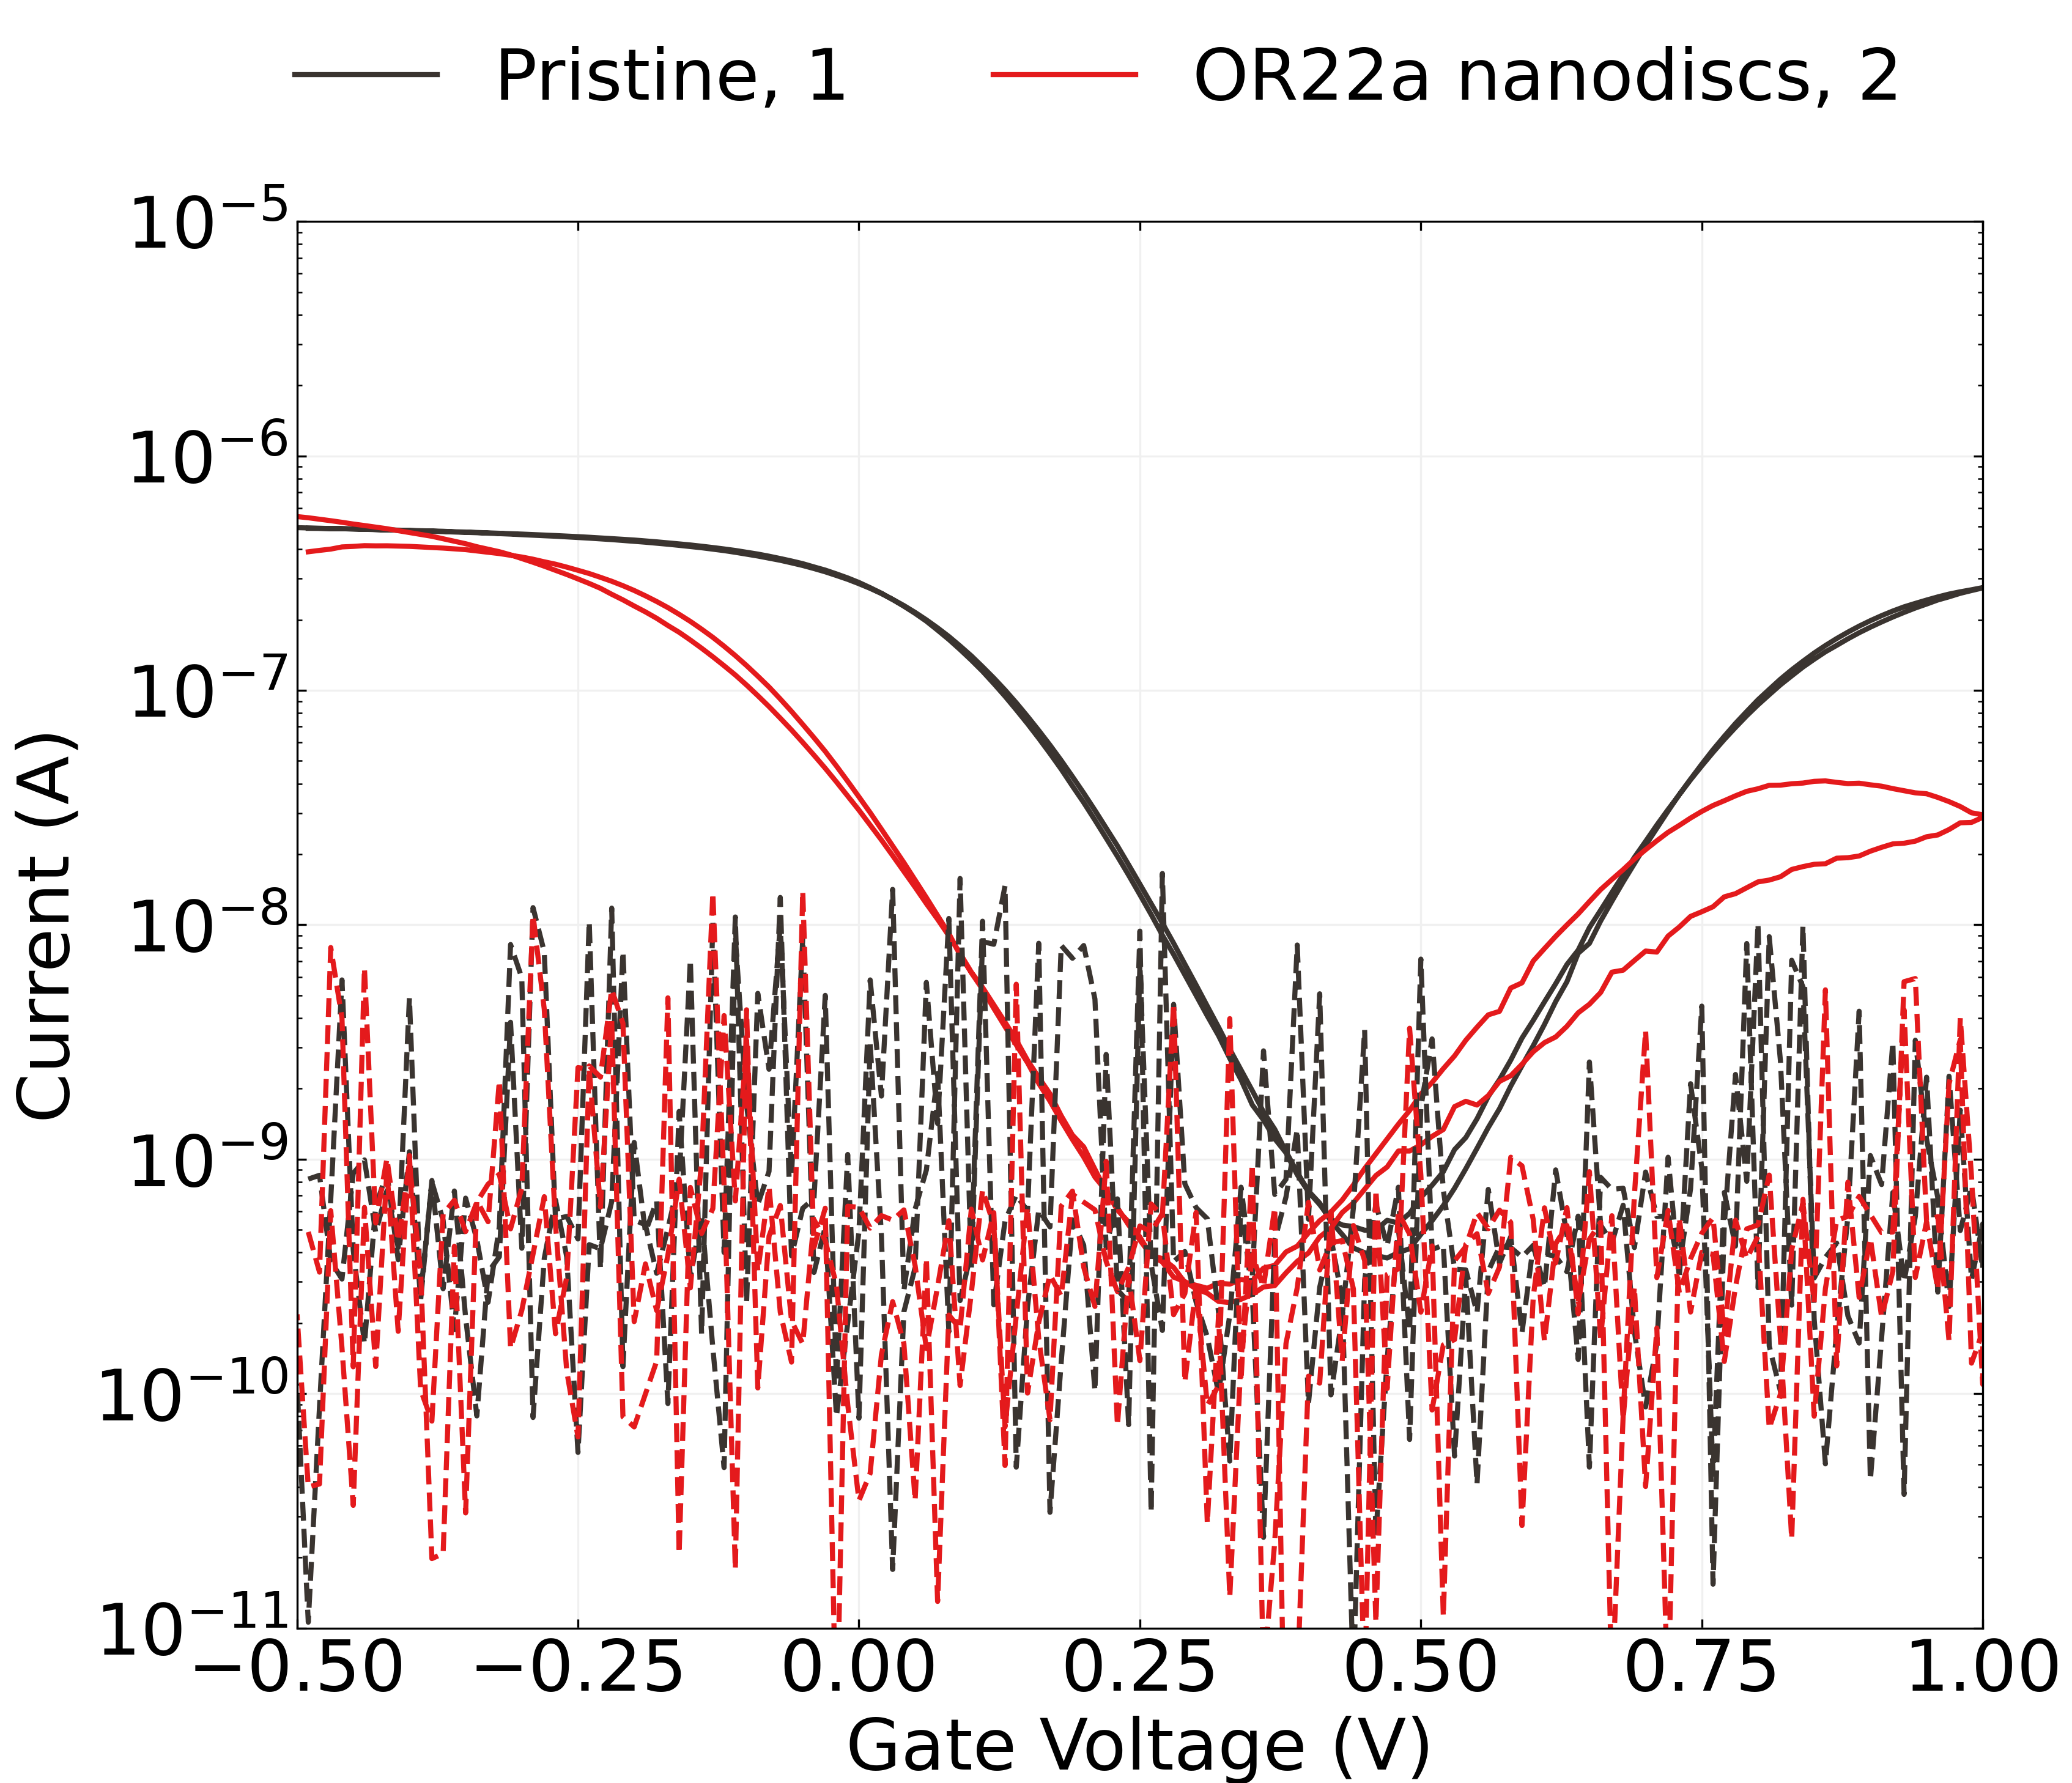
\includegraphics{figures/ch8/Q1C6_ch7_absolute_values_with_gate_current.png}

}

}

\end{minipage}%
%
\begin{minipage}[t]{0.01\linewidth}

{\centering 

~

}

\end{minipage}%
%
\begin{minipage}[t]{0.03\linewidth}

{\centering 

\raisebox{-\height}{


\includegraphics{figures/(b).png}

}

}

\end{minipage}%
%
\begin{minipage}[t]{0.01\linewidth}

{\centering 

~

}

\end{minipage}%
%
\begin{minipage}[t]{0.45\linewidth}

{\centering 

\raisebox{-\height}{

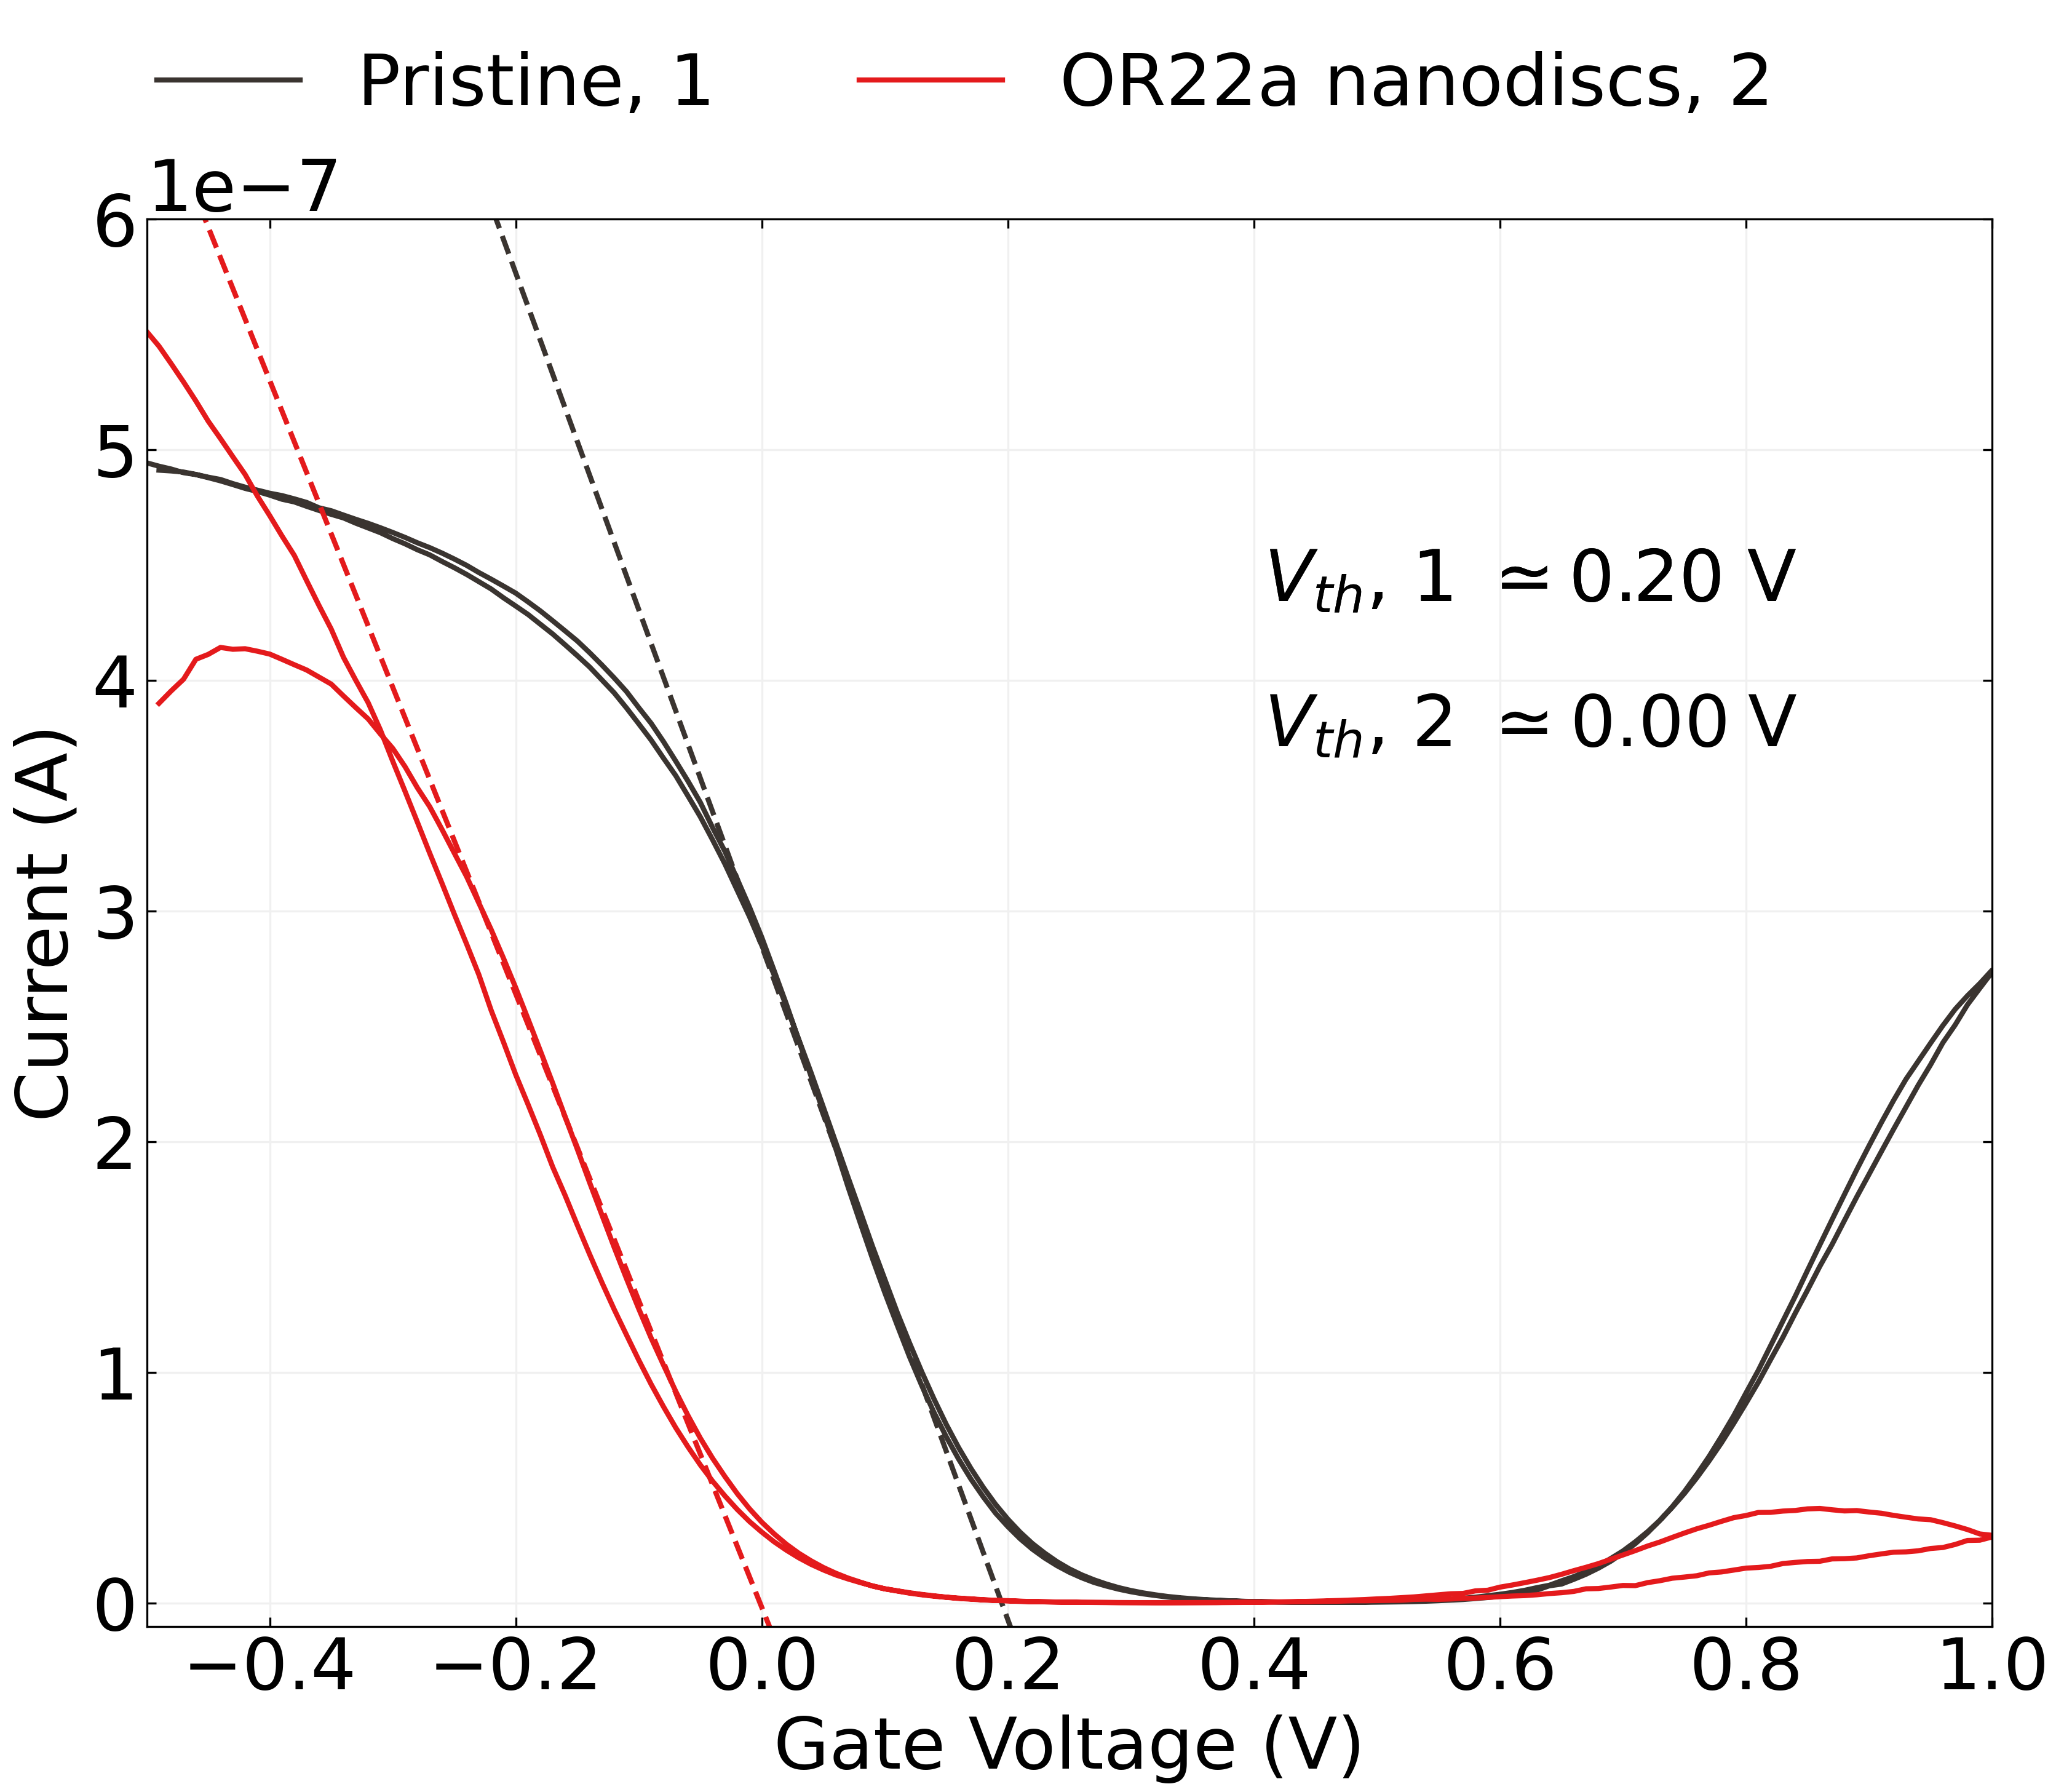
\includegraphics{figures/ch8/Q1C6_ch7_absolute_values_with_threshold_voltage_shift_without_gate_current.png}

}

}

\end{minipage}%
%
\begin{minipage}[t]{0.01\linewidth}

{\centering 

~

}

\end{minipage}%

\caption{\label{fig-OR22a-TX-comparison}Liquid-gated carbon nanotube
network device transfer characteristics before and after OR22a nanodisc
functionalisation. Source-drain current was \(V_{ds}\) = 100 mV for both
the forward and reverse sweep. In (a), the characteristics are shown on
a logarithmic scale, where the gate current for each transfer curve is
shown with a dashed line. In (b), the characteristics are shown on a
linear scale alongside a dashed line tangent to the subthreshold slope
of the characteristic curve. The threshold voltage corresponding to the
intercept of this slope with the x-axis is shown for each transfer
characteristic curve.}

\end{figure}

Liquid-gated electrical characteristics were taken of the sensing
channel (channel 7) before and after functionalisation with OR22a
nanodiscs. These electrical characteristics were taken in using a liquid
gate buffer of 1XPBS containing 0.5\% v/v DMSO with the B1500A
semiconductor device analyser. These characteristics are shown in
Figure~\ref{fig-OR22a-TX-comparison}, shown using both a logarithmic and
linear current scale. The device exhibited ambipolar characteristics
before functionalisation, which is typically seen for steam-deposited
carbon nanotube films (\textbf{?@sec-cnt-devices}). However, \(p\)-type
behaviour dominates after device functionalisation due to a significant
drop in \(n\)-type conductance. There was little hysteresis present,
which is also typical for these devices. A slight increase in hysteresis
was observed post-functionalisation. Leakage current (shown by the
dashed traces) never exceeds \(1 \times 10^{-7}\) V, both before and
after functionalisation. The significant change in electrical
characteristics observed could be due to five possible factors \(-\)
adsorption of solvent onto the network, network attachment of PBASE
without subsequent protein attachment, non-specific adsorption of
protein onto the network, PBASE-mediated attachment of the membrane
scaffold protein (MSP) of nanodiscs to the network, and PBASE-mediated
attachment of odorant receptors to the network. Note that as the
nanodisc volume is much larger than that of the odorant receptor, any
direct protein adsorption is highly likely to be adsorption of the
nanodisc membrane scaffold protein onto the carbon nanotube network.
Odorant receptor attachment via PBASE is therefore the only desirable
functionalisation result for sensing purposes.

Only minor changes were observed in the on-off ratio when comparing the
device channel before and after functionalisation. The on-off ratio for
the pristine channel was \(1120\pm220\), fairly typical for a transfer
curve from a steam-assisted surfactant-deposited CNT network device (see
\textbf{?@sec-cnt-devices}). The on-off ratio increased slightly to
\(1830\pm550\) after functionalisation. We expect to see an increase in
on-off ratio for a device successfully functionalised with OR22a
nanodiscs, which may result from an increase in negative charge causing
modulation of Schottky barriers between metallic and semiconducting
carbon nanotubes within the network \autocite{Murugathas2019b}. However,
we also expect increased hole conductance from the attachment of PBASE,
even without proteins being present
(\textbf{?@sec-PBASE-electrical-characterisation}). It is therefore
difficult to determine whether functionalisation has been successful
from the on-off ratio of transfer characteristics alone.

Functionalisation of the channel resulted in a negative shift in
threshold voltage of \(-0.20\pm0.03\) V. This is significantly in excess
of threshold voltage shifts measured for both methanol adsorption
(\(-0.15\pm0.02\) V) and after exposure to PBASE in methanol
(\(-0.06\pm0.04\) V), confirming that protein has attached to the carbon
nanotubes. However, both direct protein adsorption
\autocite{Bradley2004,Heller2008} and empty nanodisc attachment
\autocite{Murugathas2019b} should also lead to a significant negative
threshold voltage shift in the liquid-gated transfer characteristic
curve. In all three cases, the voltage shift is predominantly the result
of negative charge transfer from the adsorped proteins to the
semiconducting carbon nanotubes
\autocite{Bradley2004,Heller2008,Murugathas2019b}. It is likely that the
negative shift observed results from some combination of the three types
of attachment. It should be noted that while the size of the
functionalisation-induced threshold voltage shift can be used to
determine whether protein has attached to the nanodisc network, it
cannot be used to specifically determine whether odorant receptors have
attached to the network.

\begin{figure}

\begin{minipage}[t]{0.03\linewidth}

{\centering 

\raisebox{-\height}{


\includegraphics{figures/(a).png}

}

}

\end{minipage}%
%
\begin{minipage}[t]{0.01\linewidth}

{\centering 

~

}

\end{minipage}%
%
\begin{minipage}[t]{0.45\linewidth}

{\centering 

\raisebox{-\height}{

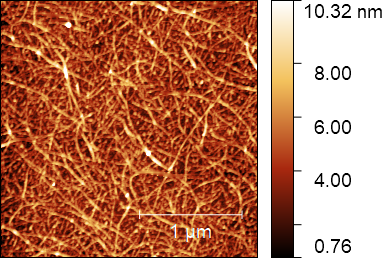
\includegraphics{figures/ch8/Pristine_DF2Q3D10_ 00141.png}

}

}

\end{minipage}%
%
\begin{minipage}[t]{0.01\linewidth}

{\centering 

~

}

\end{minipage}%
%
\begin{minipage}[t]{0.03\linewidth}

{\centering 

\raisebox{-\height}{


\includegraphics{figures/(b).png}

}

}

\end{minipage}%
%
\begin{minipage}[t]{0.01\linewidth}

{\centering 

~

}

\end{minipage}%
%
\begin{minipage}[t]{0.45\linewidth}

{\centering 

\raisebox{-\height}{

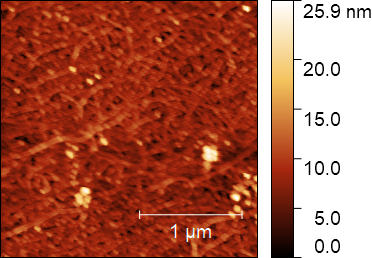
\includegraphics{figures/ch8/DF2Q1D6_postNDOR22a_ch7_1_00375.png}

}

}

\end{minipage}%
%
\begin{minipage}[t]{0.01\linewidth}

{\centering 

~

}

\end{minipage}%

\caption{\label{fig-working-OR22a-AFM}Atomic force microscope images of
the channel region of carbon nanotube network devices before and after
functionalisation. The channel network of a pristine device is shown in
(a), while (b) is of channel 7 from the sensing device functionalised in
this section.}

\end{figure}

Atomic force microscope images of the device channels both before
functionalisation and after sensing with the functionalised device to
confirm the presence of nanodiscs. As far as the author knows, these are
the first atomic force microscope images taken of iOR nanodiscs found on
a sensing channel rather than on a separate carbon nanotube film; this
was made possible by using the 20 µm wide aperture encapsulation mask
discussed in \textbf{?@sec-encapsulation}. These images are shown in
Figure~\ref{fig-working-OR22a-AFM}. Aggregations of nanodiscs are
visible in Figure~\ref{fig-working-OR22a-AFM} (c)\(-\)(d). These
nanodisc clusters are especially sizable in the lower half of
Figure~\ref{fig-working-OR22a-AFM} (c), where the two largest clusters
are \(200\pm10\) nm across at their widest point. However, these
features are still much smaller than most of the agglomerated nanodisc
features seen by Murugathas \emph{et al.} \autocite{Murugathas2019b}.
Furthermore, the nanodisc features closely follow the carbon nanotube
bundles across the densely bundled morphology used by Murugathas
\emph{et al.} \autocite{Murugathas2019b}. On the dense network
morphology used here, the position of nanodisc clusters relative to the
carbon nanotubes is less distinct. To confirm whether nanodiscs have
preferentially attached to the carbon nanotubes, a more quantitative
approach is needed.

\begin{figure}

\begin{minipage}[t]{0.03\linewidth}

{\centering 

\raisebox{-\height}{


\includegraphics{figures/(a).png}

}

}

\end{minipage}%
%
\begin{minipage}[t]{0.01\linewidth}

{\centering 

~

}

\end{minipage}%
%
\begin{minipage}[t]{0.45\linewidth}

{\centering 

\raisebox{-\height}{

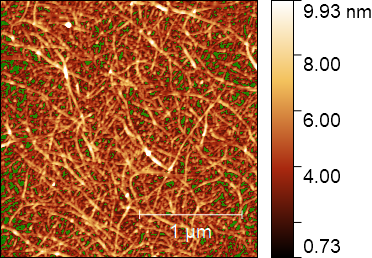
\includegraphics{figures/ch8/Pristine_DF2Q3D10_00141_mask.png}

}

}

\end{minipage}%
%
\begin{minipage}[t]{0.01\linewidth}

{\centering 

~

}

\end{minipage}%
%
\begin{minipage}[t]{0.03\linewidth}

{\centering 

\raisebox{-\height}{


\includegraphics{figures/(b).png}

}

}

\end{minipage}%
%
\begin{minipage}[t]{0.01\linewidth}

{\centering 

~

}

\end{minipage}%
%
\begin{minipage}[t]{0.45\linewidth}

{\centering 

\raisebox{-\height}{

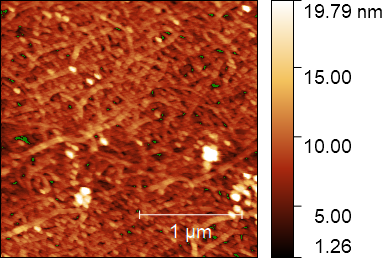
\includegraphics{figures/ch8/DF2Q1D6_postNDOR22a_ch7_1_00375_mask.png}

}

}

\end{minipage}%
%
\begin{minipage}[t]{0.01\linewidth}

{\centering 

~

}

\end{minipage}%

\caption{\label{fig-working-OR22a-masks}Atomic force microscope images
with the substrate background highlighted with a green mask. Here, (a)
shows a device channel after functionalisation with PBASE and methanol,
while (b) shows channel 7 from the sensing device functionalised with
OR22a nanodiscs in this section.}

\end{figure}

The average height of the substrate was found for both pristine and
functionalised atomic force microscope images using the masking tool in
Gwyddion. The masks for each image are shown in
Figure~\ref{fig-working-OR22a-masks}. Average substrate heights of
\(1.9\pm0.3\) nm and \(3.3\pm0.4\) nm were found for the pristine and
functionalised networks respectively. In Gwyddion, both networks were
simplified to a binary representation, where features above a certain
threshold were shown as white and features below shown as black. This
representation, shown in Figure~\ref{fig-crosssection}, has the
appearance of a cross-section through the network at the threshold
height. The threshold was chosen as the minimum height where carbon
nanotube spindles were no longer apparent in the functionalised image,
8.7 nm above the substrate. Figure~\ref{fig-crosssection} (a) shows only
a few, sparsely distributed features, the majority of which are below 50
nm in width. These features may correspond to large nanotube-nanotube
junctions, surfactant residue, or other surface contamination
(\textbf{?@sec-pristine-morphology}). In Figure~\ref{fig-crosssection}
(b), many features are over 50 nm across. They are often found close
together, and form a curved line across the network in the bottom left
corner (shown in red); this curvilinear arrangement of nanodisc features
gives a strong indication specific attachment to the carbon nanotubes
has occurred.

\begin{figure}

\begin{minipage}[t]{0.03\linewidth}

{\centering 

\raisebox{-\height}{


\includegraphics{figures/(a).png}

}

}

\end{minipage}%
%
\begin{minipage}[t]{0.01\linewidth}

{\centering 

~

}

\end{minipage}%
%
\begin{minipage}[t]{0.45\linewidth}

{\centering 

\raisebox{-\height}{

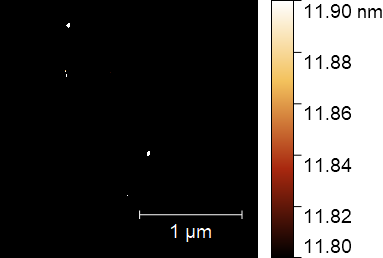
\includegraphics{figures/ch8/Pristine_DF2Q3D10_00141_crosssection.png}

}

}

\end{minipage}%
%
\begin{minipage}[t]{0.01\linewidth}

{\centering 

~

}

\end{minipage}%
%
\begin{minipage}[t]{0.03\linewidth}

{\centering 

\raisebox{-\height}{


\includegraphics{figures/(b).png}

}

}

\end{minipage}%
%
\begin{minipage}[t]{0.01\linewidth}

{\centering 

~

}

\end{minipage}%
%
\begin{minipage}[t]{0.45\linewidth}

{\centering 

\raisebox{-\height}{

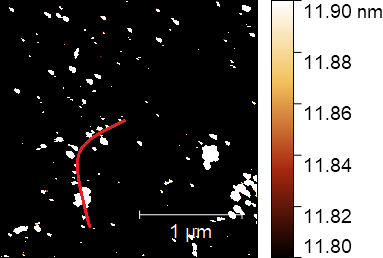
\includegraphics{figures/ch8/DF2Q1D6_postNDOR22a_ch7_1_00375_crosssection_edit.png}

}

}

\end{minipage}%
%
\begin{minipage}[t]{0.01\linewidth}

{\centering 

~

}

\end{minipage}%

\caption{\label{fig-crosssection}Binary representations of the atomic
force microscope images of (a) the pristine device, with a threshold
height of 10.6 nm, and (b) the functionalised device, with a threshold
height of 12.0 nm. Both thresholds are 8.7 nm above the substrate
background of their respective images.}

\end{figure}

As the maximum height of the functionalised AFM is 25.9 nm and only
nanodisc features are present at 12.0 nm, there must be nanodisc
agglomerates present at least 13.9 nm tall. The estimated height range
for nanodiscs is \(\sim\) 10 \(-\) 20 nm
\autocite{Nath2007,Bayburt2010,Murugathas2020}. Assuming a average
carbon nanotube height of 1.45 nm, with a average substrate height of
3.3 nm, the nanodisc agglomerations could be up to \(\sim\) 21 nm tall.
Note that height measurements of biological samples taken via AFM have
been shown to underestimate actual feature height by over 50\%
\autocite{Vobornik2023}. Even so, the breadths of the nanodisc features
are significantly greater than their heights. While the cross-sections
of the largest features are up to 20 nanodiscs across, they are a few
nanodiscs high at most; certainly less than five. It appears that,
rather than clustering together in solution and attaching as an
aggregate, the nanodiscs are individually attaching to preferred
locations on the network. These locations may be at junctions between
two large carbon nanotubes, which have a relatively large surface area
available for binding, or at locations particularly clean of
contamination. AFM images showing iOR-nanodisc functionalised carbon
nanotube networks with significant vertical clustering have been
reported, but these images were not of channels used for sensing
\autocite{Murugathas2019b}.

\begin{figure}

\begin{minipage}[t]{0.03\linewidth}

{\centering 

\raisebox{-\height}{


\includegraphics{figures/(a).png}

}

}

\end{minipage}%
%
\begin{minipage}[t]{0.01\linewidth}

{\centering 

~

}

\end{minipage}%
%
\begin{minipage}[t]{0.45\linewidth}

{\centering 

\raisebox{-\height}{

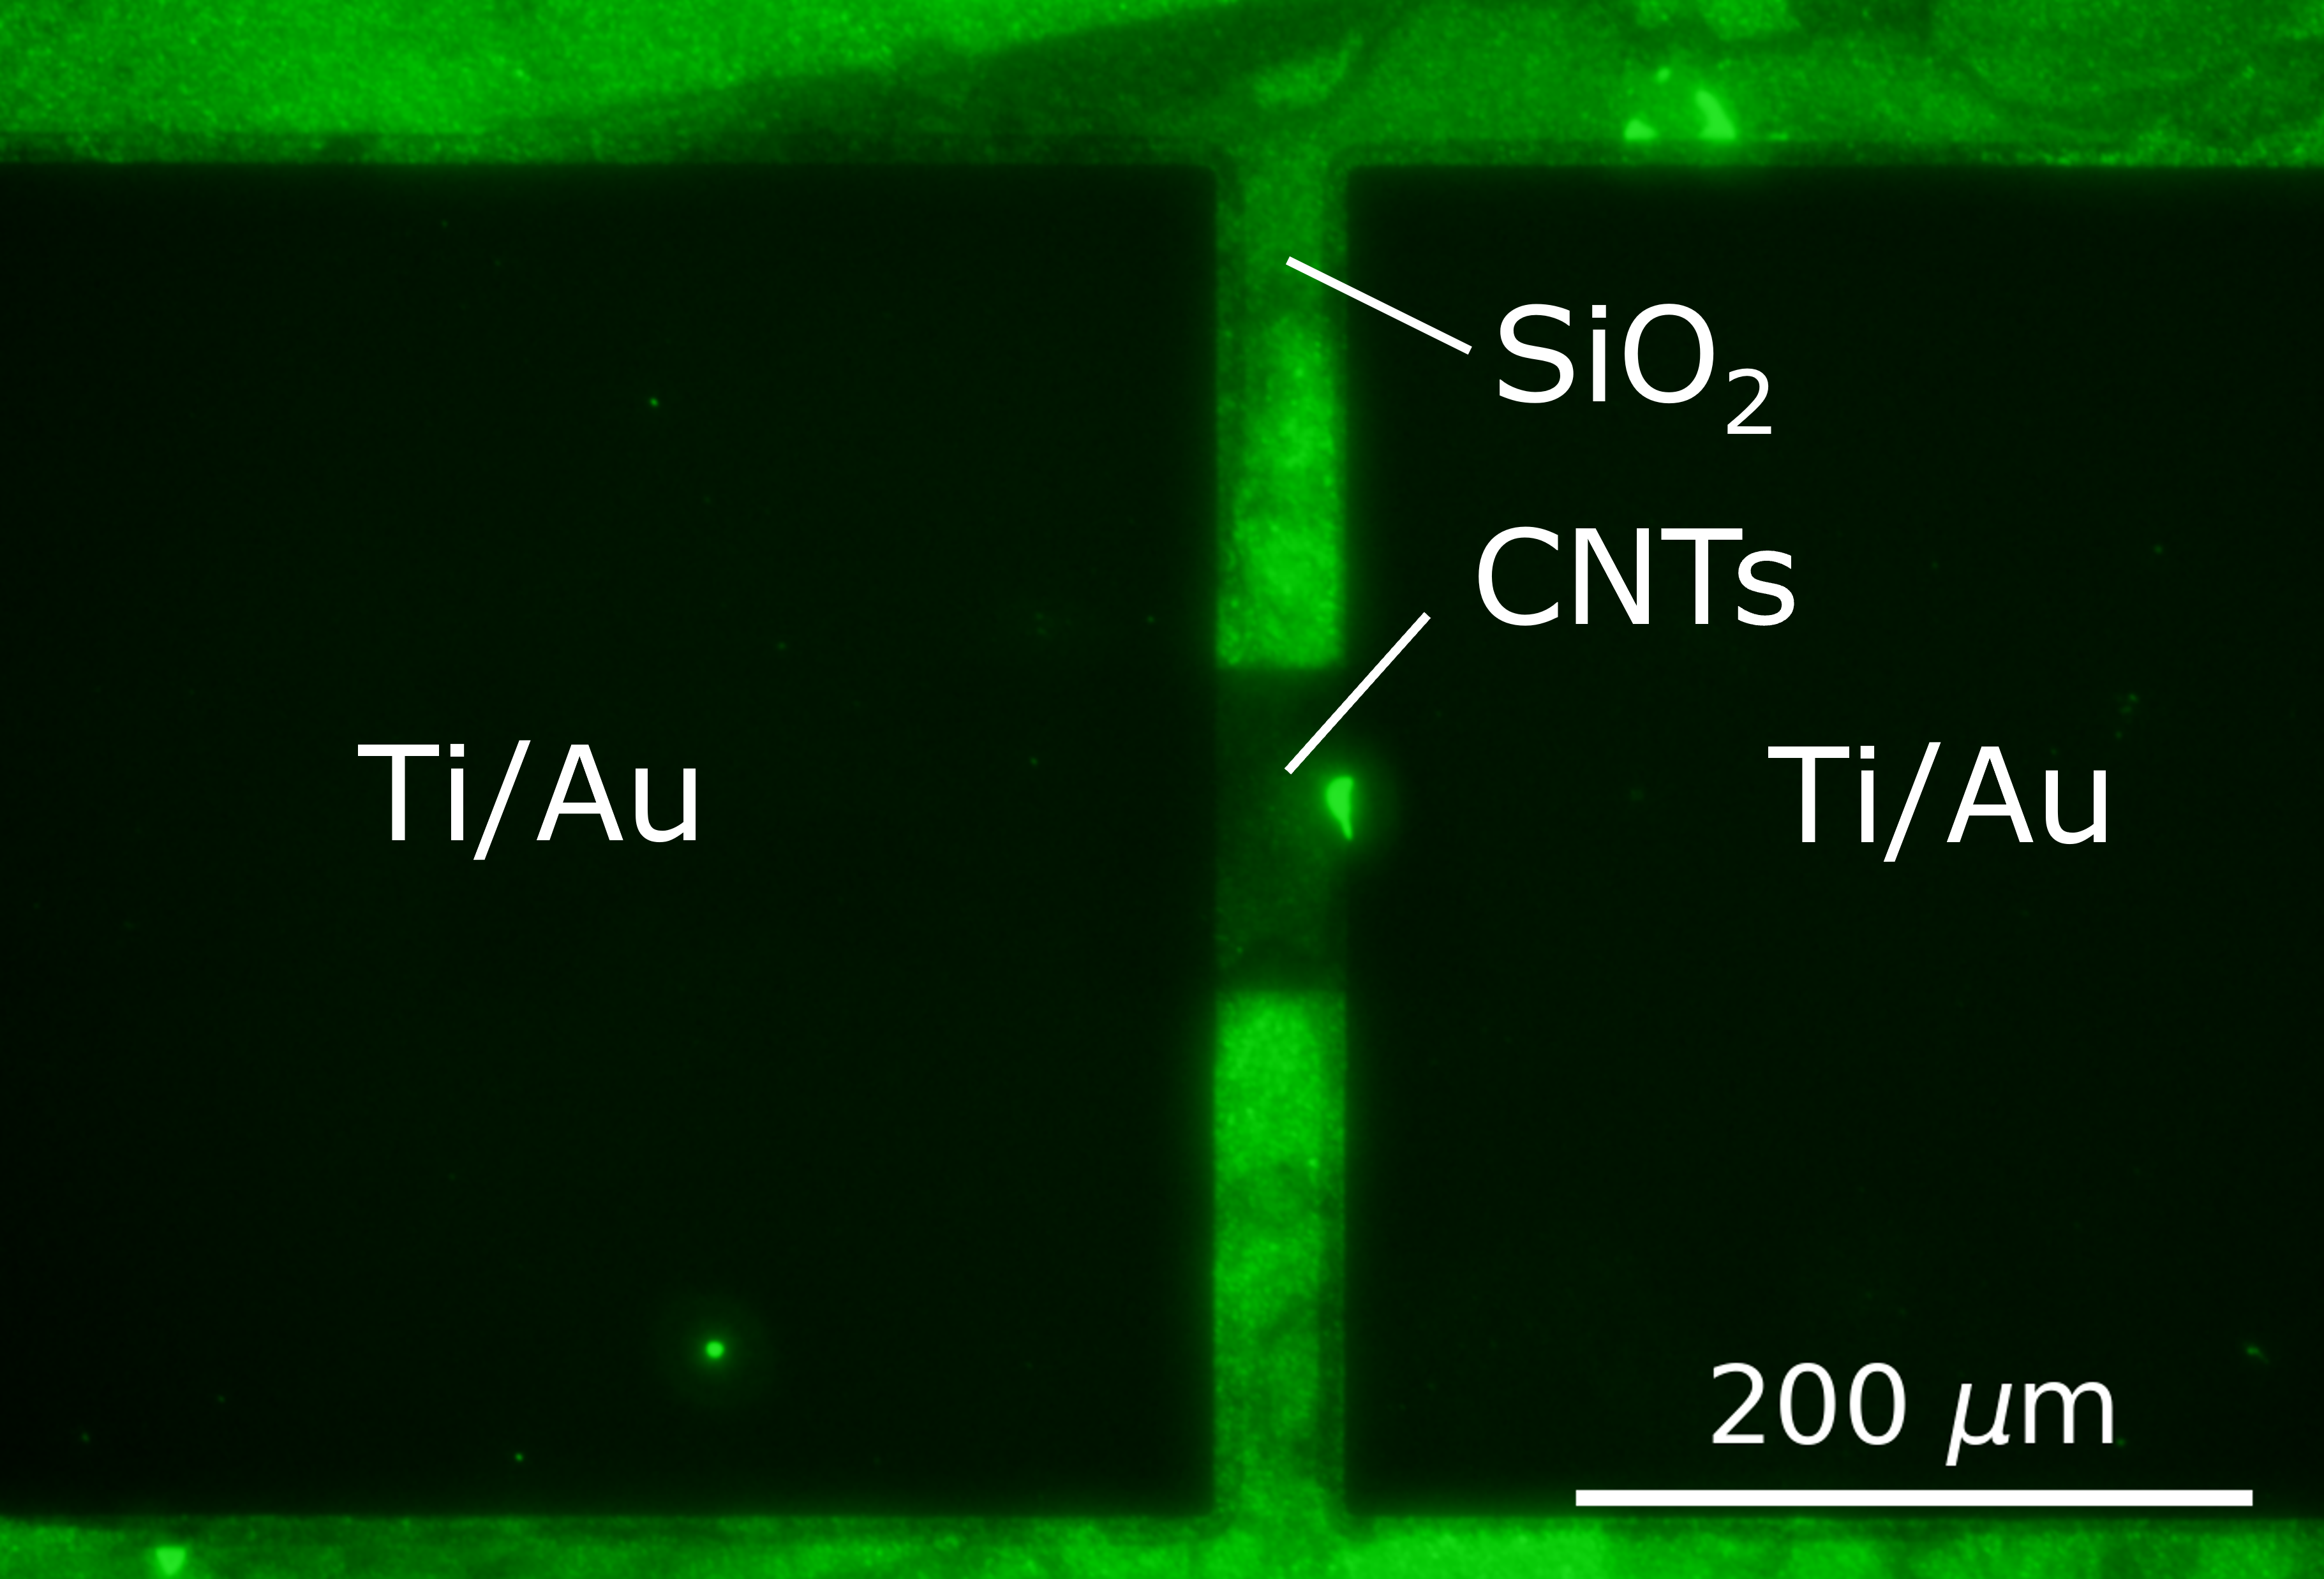
\includegraphics{figures/ch8/modified_GFPOR_10sexposure_20X_mediumcontrast_ch6_240208.png}

}

}

\end{minipage}%
%
\begin{minipage}[t]{0.01\linewidth}

{\centering 

~

}

\end{minipage}%
%
\begin{minipage}[t]{0.03\linewidth}

{\centering 

\raisebox{-\height}{


\includegraphics{figures/(b).png}

}

}

\end{minipage}%
%
\begin{minipage}[t]{0.01\linewidth}

{\centering 

~

}

\end{minipage}%
%
\begin{minipage}[t]{0.45\linewidth}

{\centering 

\raisebox{-\height}{

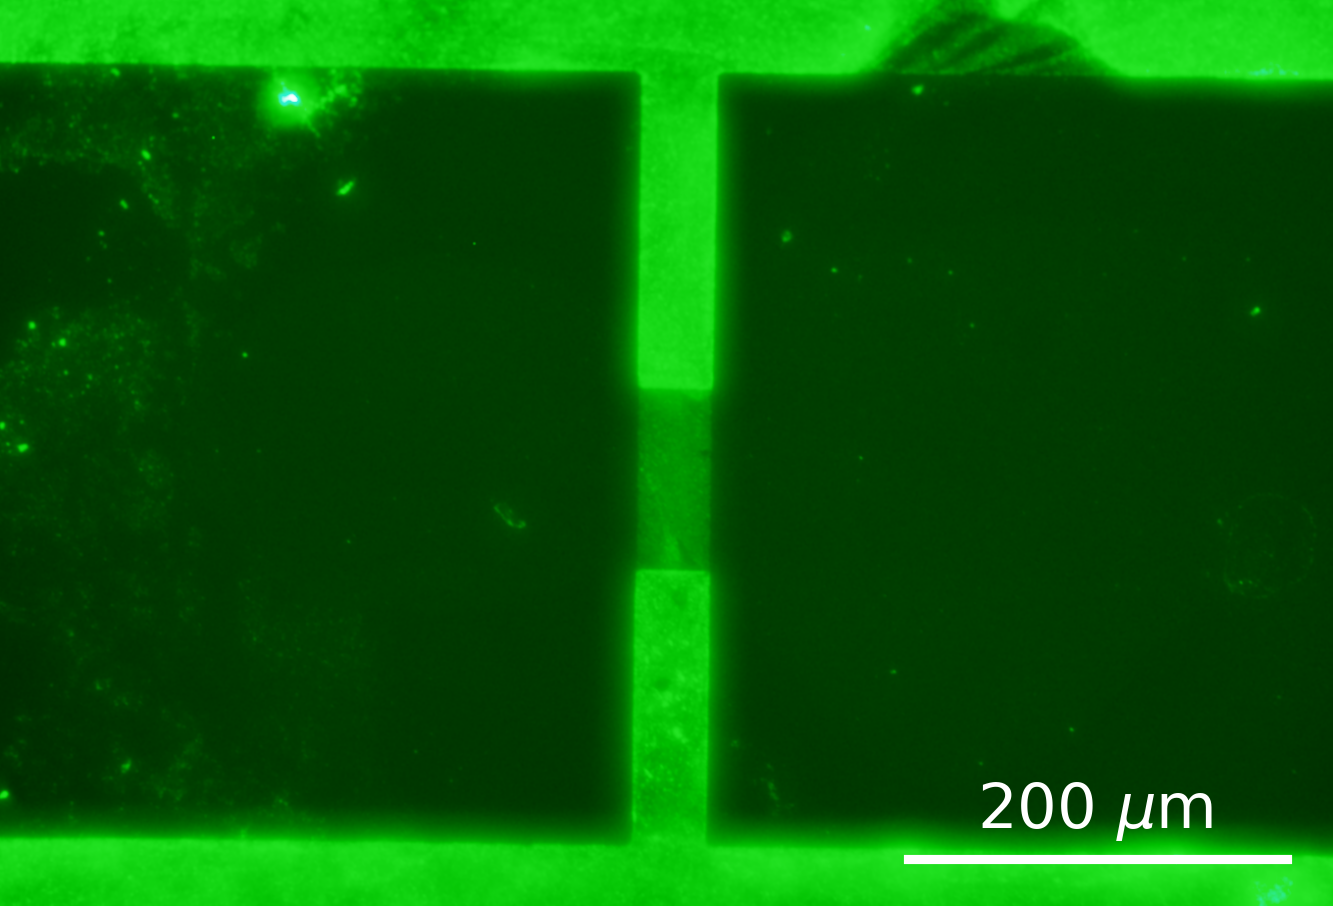
\includegraphics{figures/ch8/modified_GFPOR_PBASE_10sexposure_20X_mediumcontrast_ch1_231019_2.png}

}

}

\end{minipage}%
%
\begin{minipage}[t]{0.01\linewidth}

{\centering 

~

}

\end{minipage}%
\newline
\begin{minipage}[t]{0.03\linewidth}

{\centering 

\raisebox{-\height}{


\includegraphics{figures/(c).png}

}

}

\end{minipage}%
%
\begin{minipage}[t]{0.01\linewidth}

{\centering 

~

}

\end{minipage}%
%
\begin{minipage}[t]{0.45\linewidth}

{\centering 

\raisebox{-\height}{

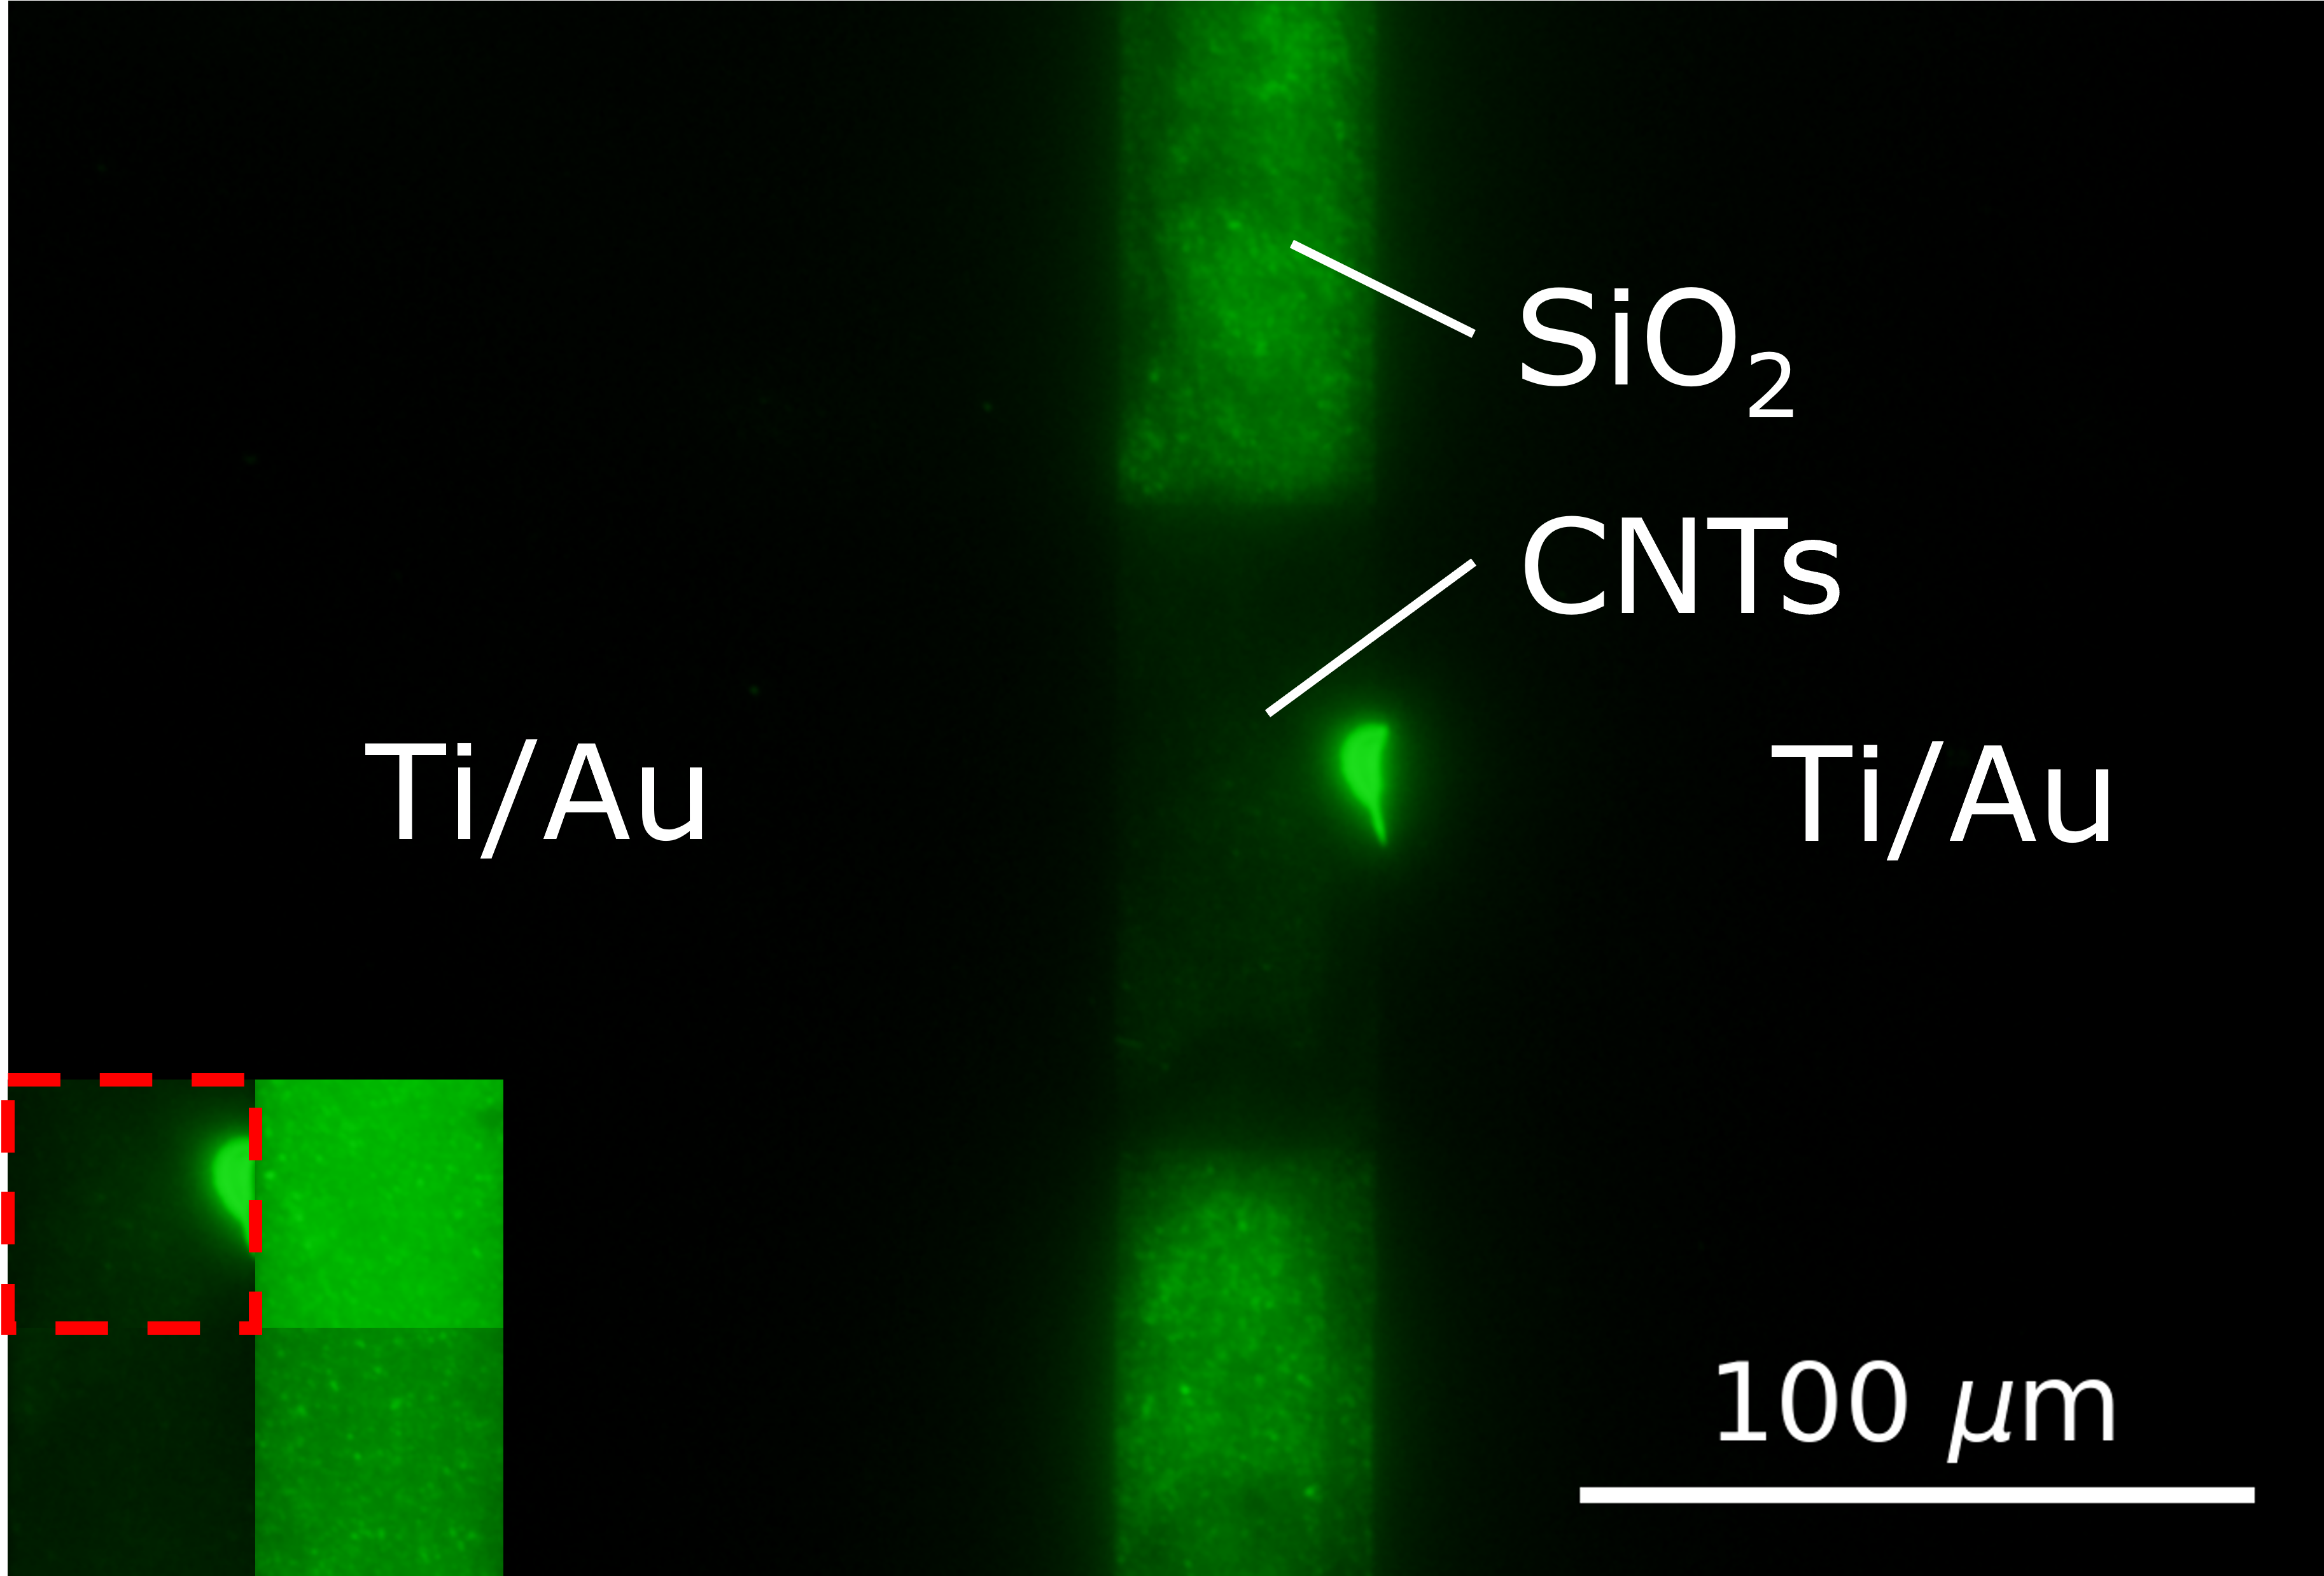
\includegraphics{figures/ch8/modified_GFPOR_10sexposure_40X_mediumcontrast_ch6_240208.png}

}

}

\end{minipage}%
%
\begin{minipage}[t]{0.01\linewidth}

{\centering 

~

}

\end{minipage}%
%
\begin{minipage}[t]{0.03\linewidth}

{\centering 

\raisebox{-\height}{


\includegraphics{figures/(d).png}

}

}

\end{minipage}%
%
\begin{minipage}[t]{0.01\linewidth}

{\centering 

~

}

\end{minipage}%
%
\begin{minipage}[t]{0.45\linewidth}

{\centering 

\raisebox{-\height}{

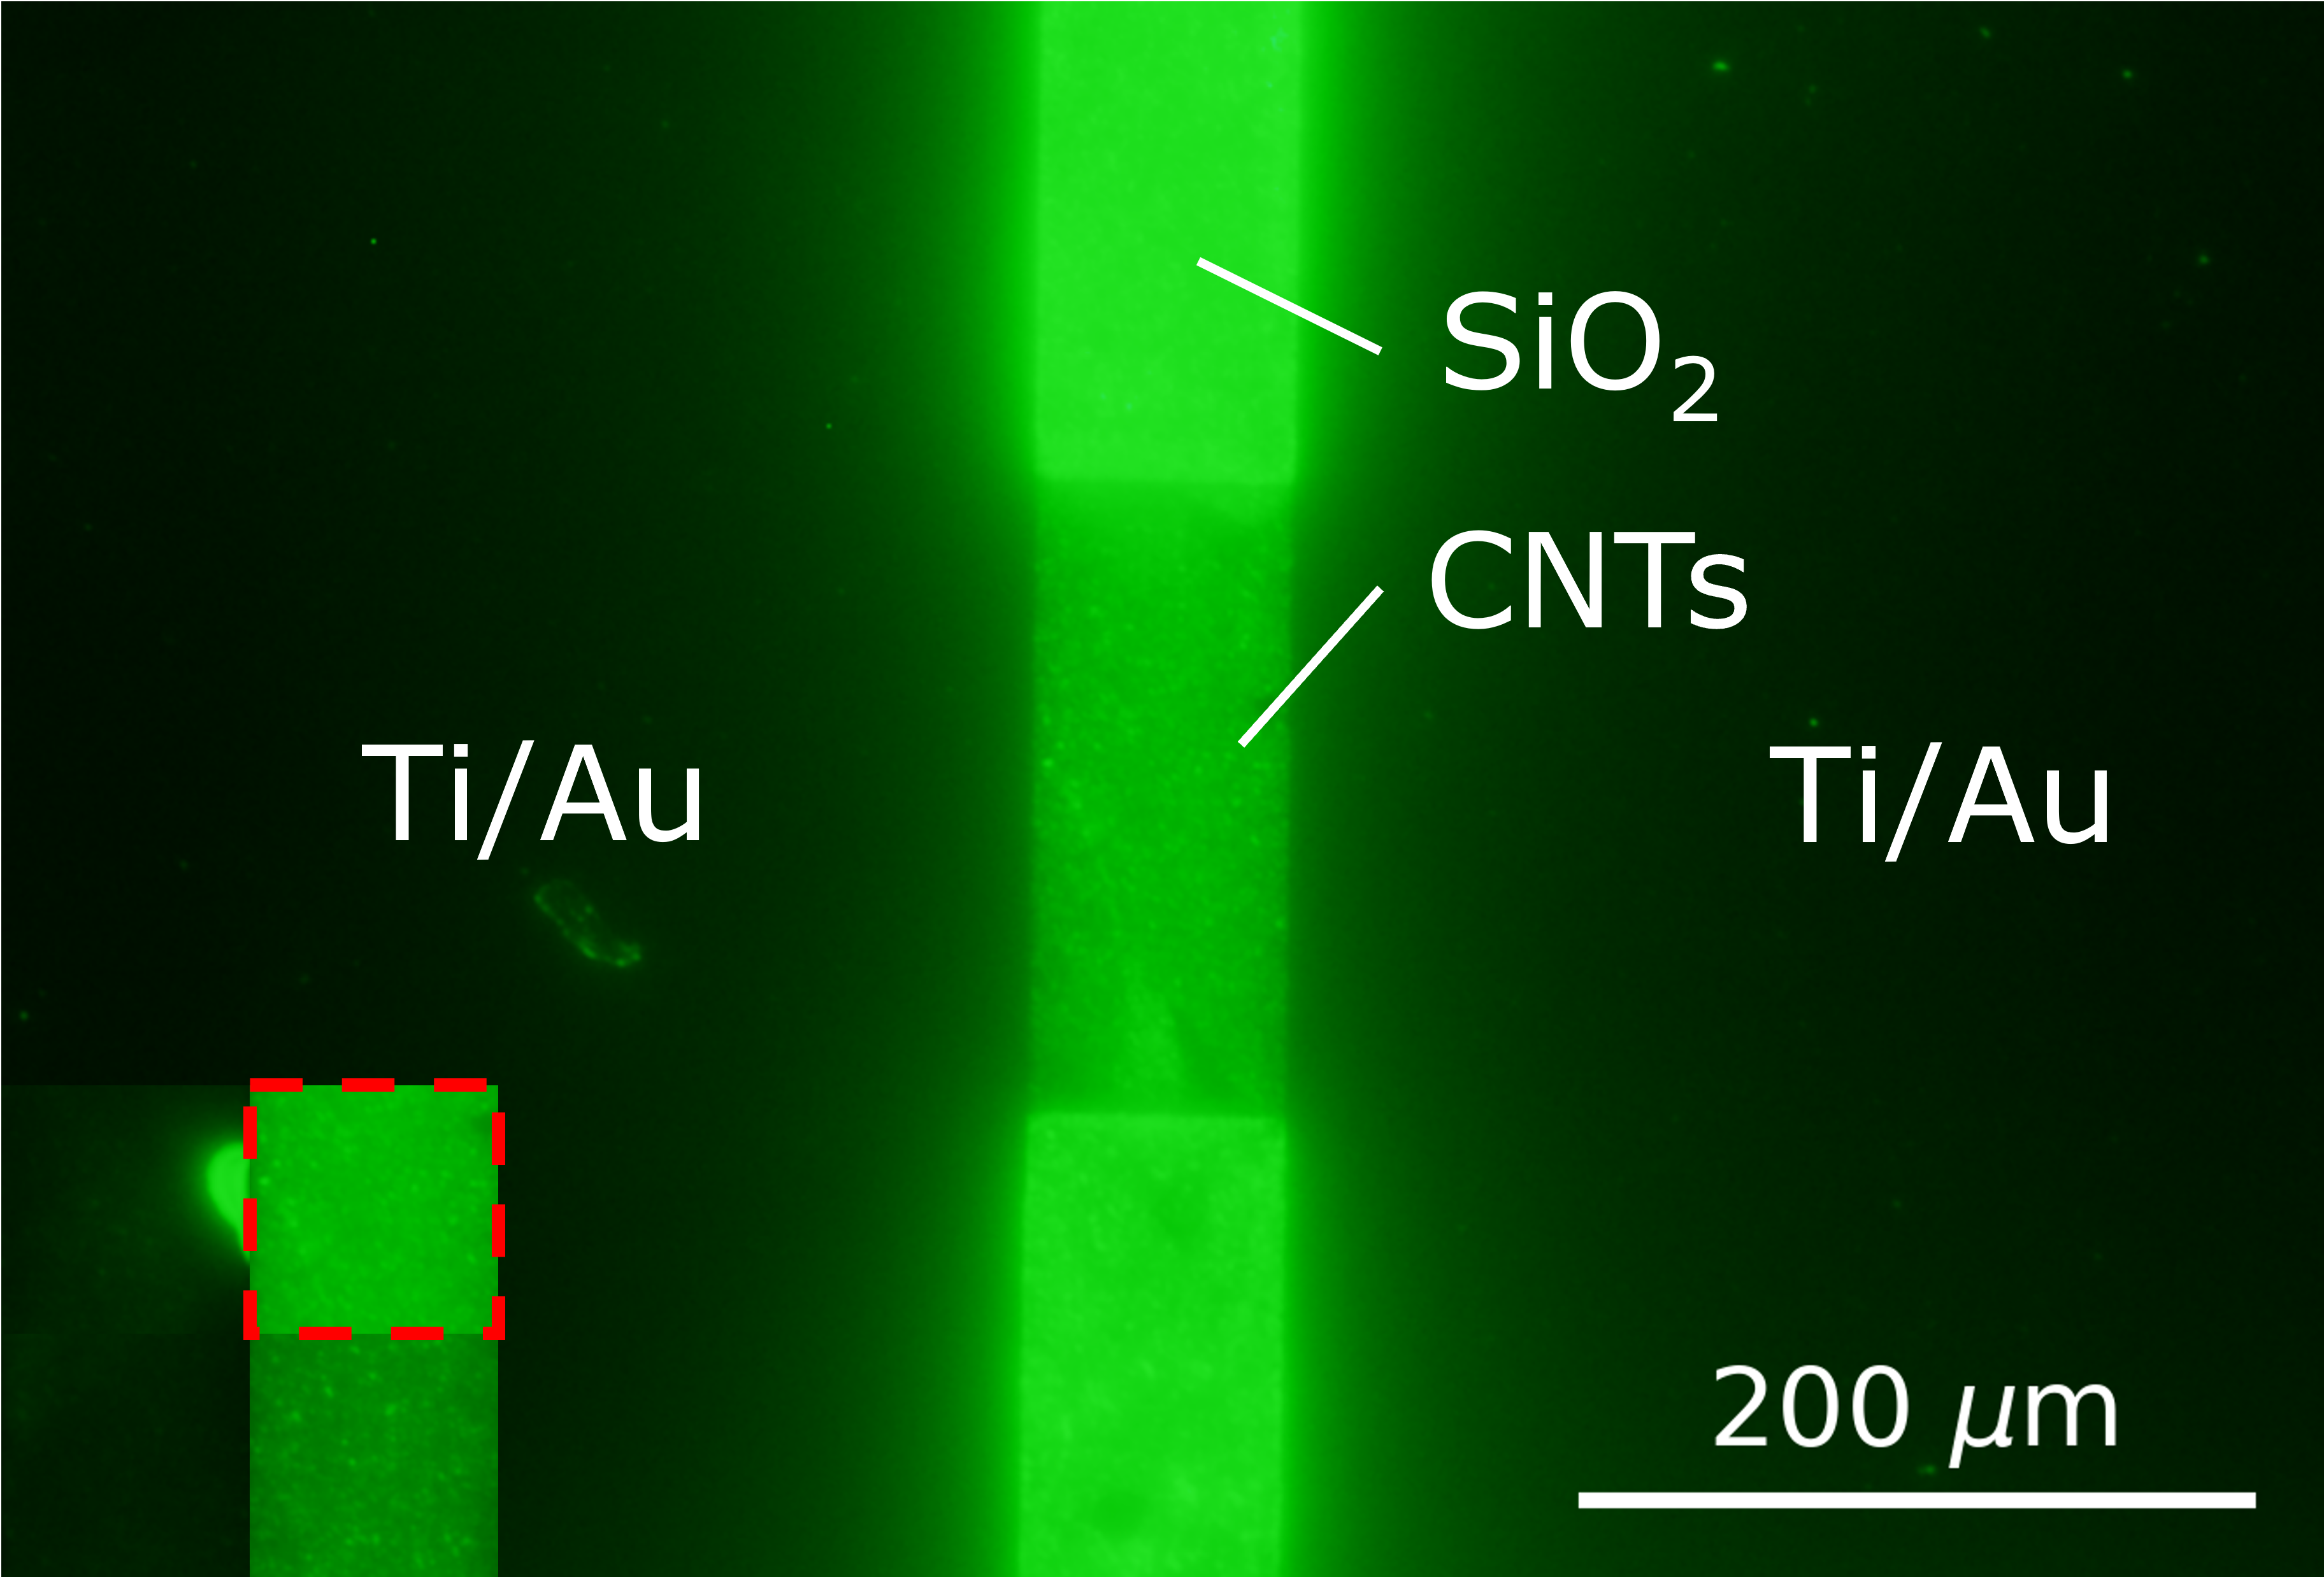
\includegraphics{figures/ch8/modified_GFPOR_PBASE_10sexposure_40X_mediumcontrast_ch1_231019_2.png}

}

}

\end{minipage}%
%
\begin{minipage}[t]{0.01\linewidth}

{\centering 

~

}

\end{minipage}%
\newline
\begin{minipage}[t]{0.03\linewidth}

{\centering 

\raisebox{-\height}{


\includegraphics{figures/(e).png}

}

}

\end{minipage}%
%
\begin{minipage}[t]{0.01\linewidth}

{\centering 

~

}

\end{minipage}%
%
\begin{minipage}[t]{0.45\linewidth}

{\centering 

\raisebox{-\height}{

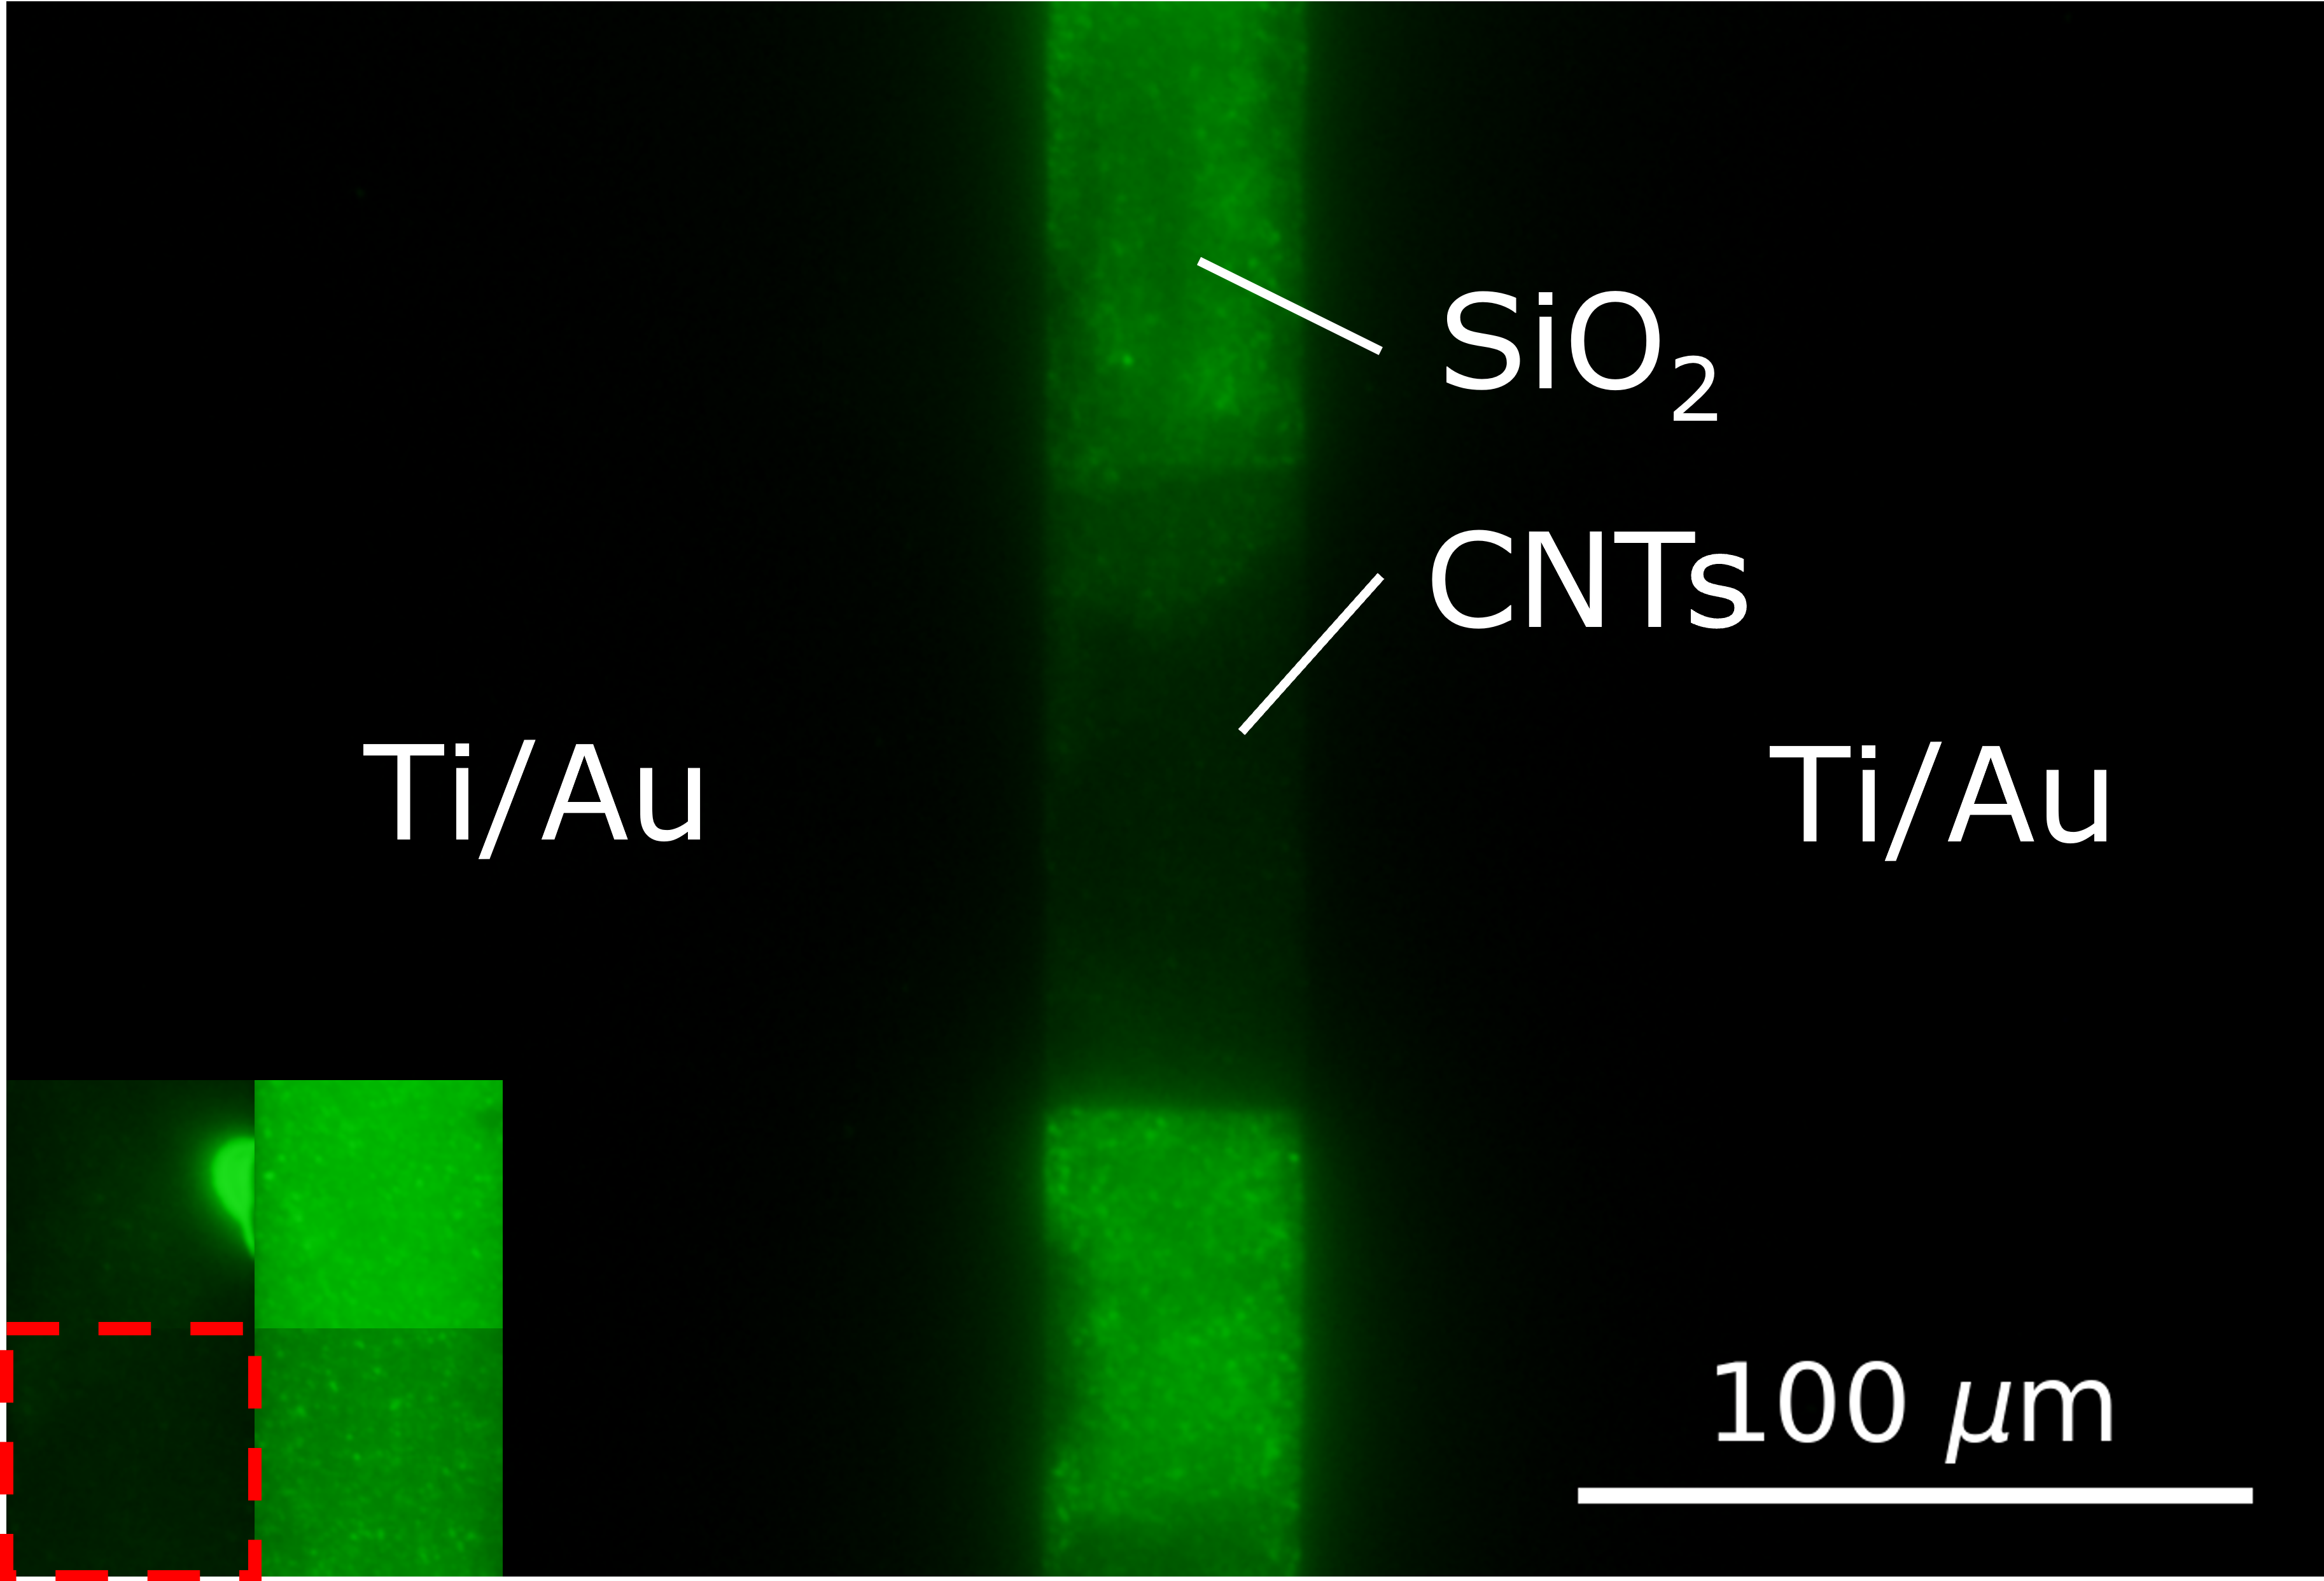
\includegraphics{figures/ch8/modified_GFPOR_10sexposure_40X_mediumcontrast_ch3_240208.png}

}

}

\end{minipage}%
%
\begin{minipage}[t]{0.01\linewidth}

{\centering 

~

}

\end{minipage}%
%
\begin{minipage}[t]{0.03\linewidth}

{\centering 

\raisebox{-\height}{


\includegraphics{figures/(f).png}

}

}

\end{minipage}%
%
\begin{minipage}[t]{0.01\linewidth}

{\centering 

~

}

\end{minipage}%
%
\begin{minipage}[t]{0.45\linewidth}

{\centering 

\raisebox{-\height}{

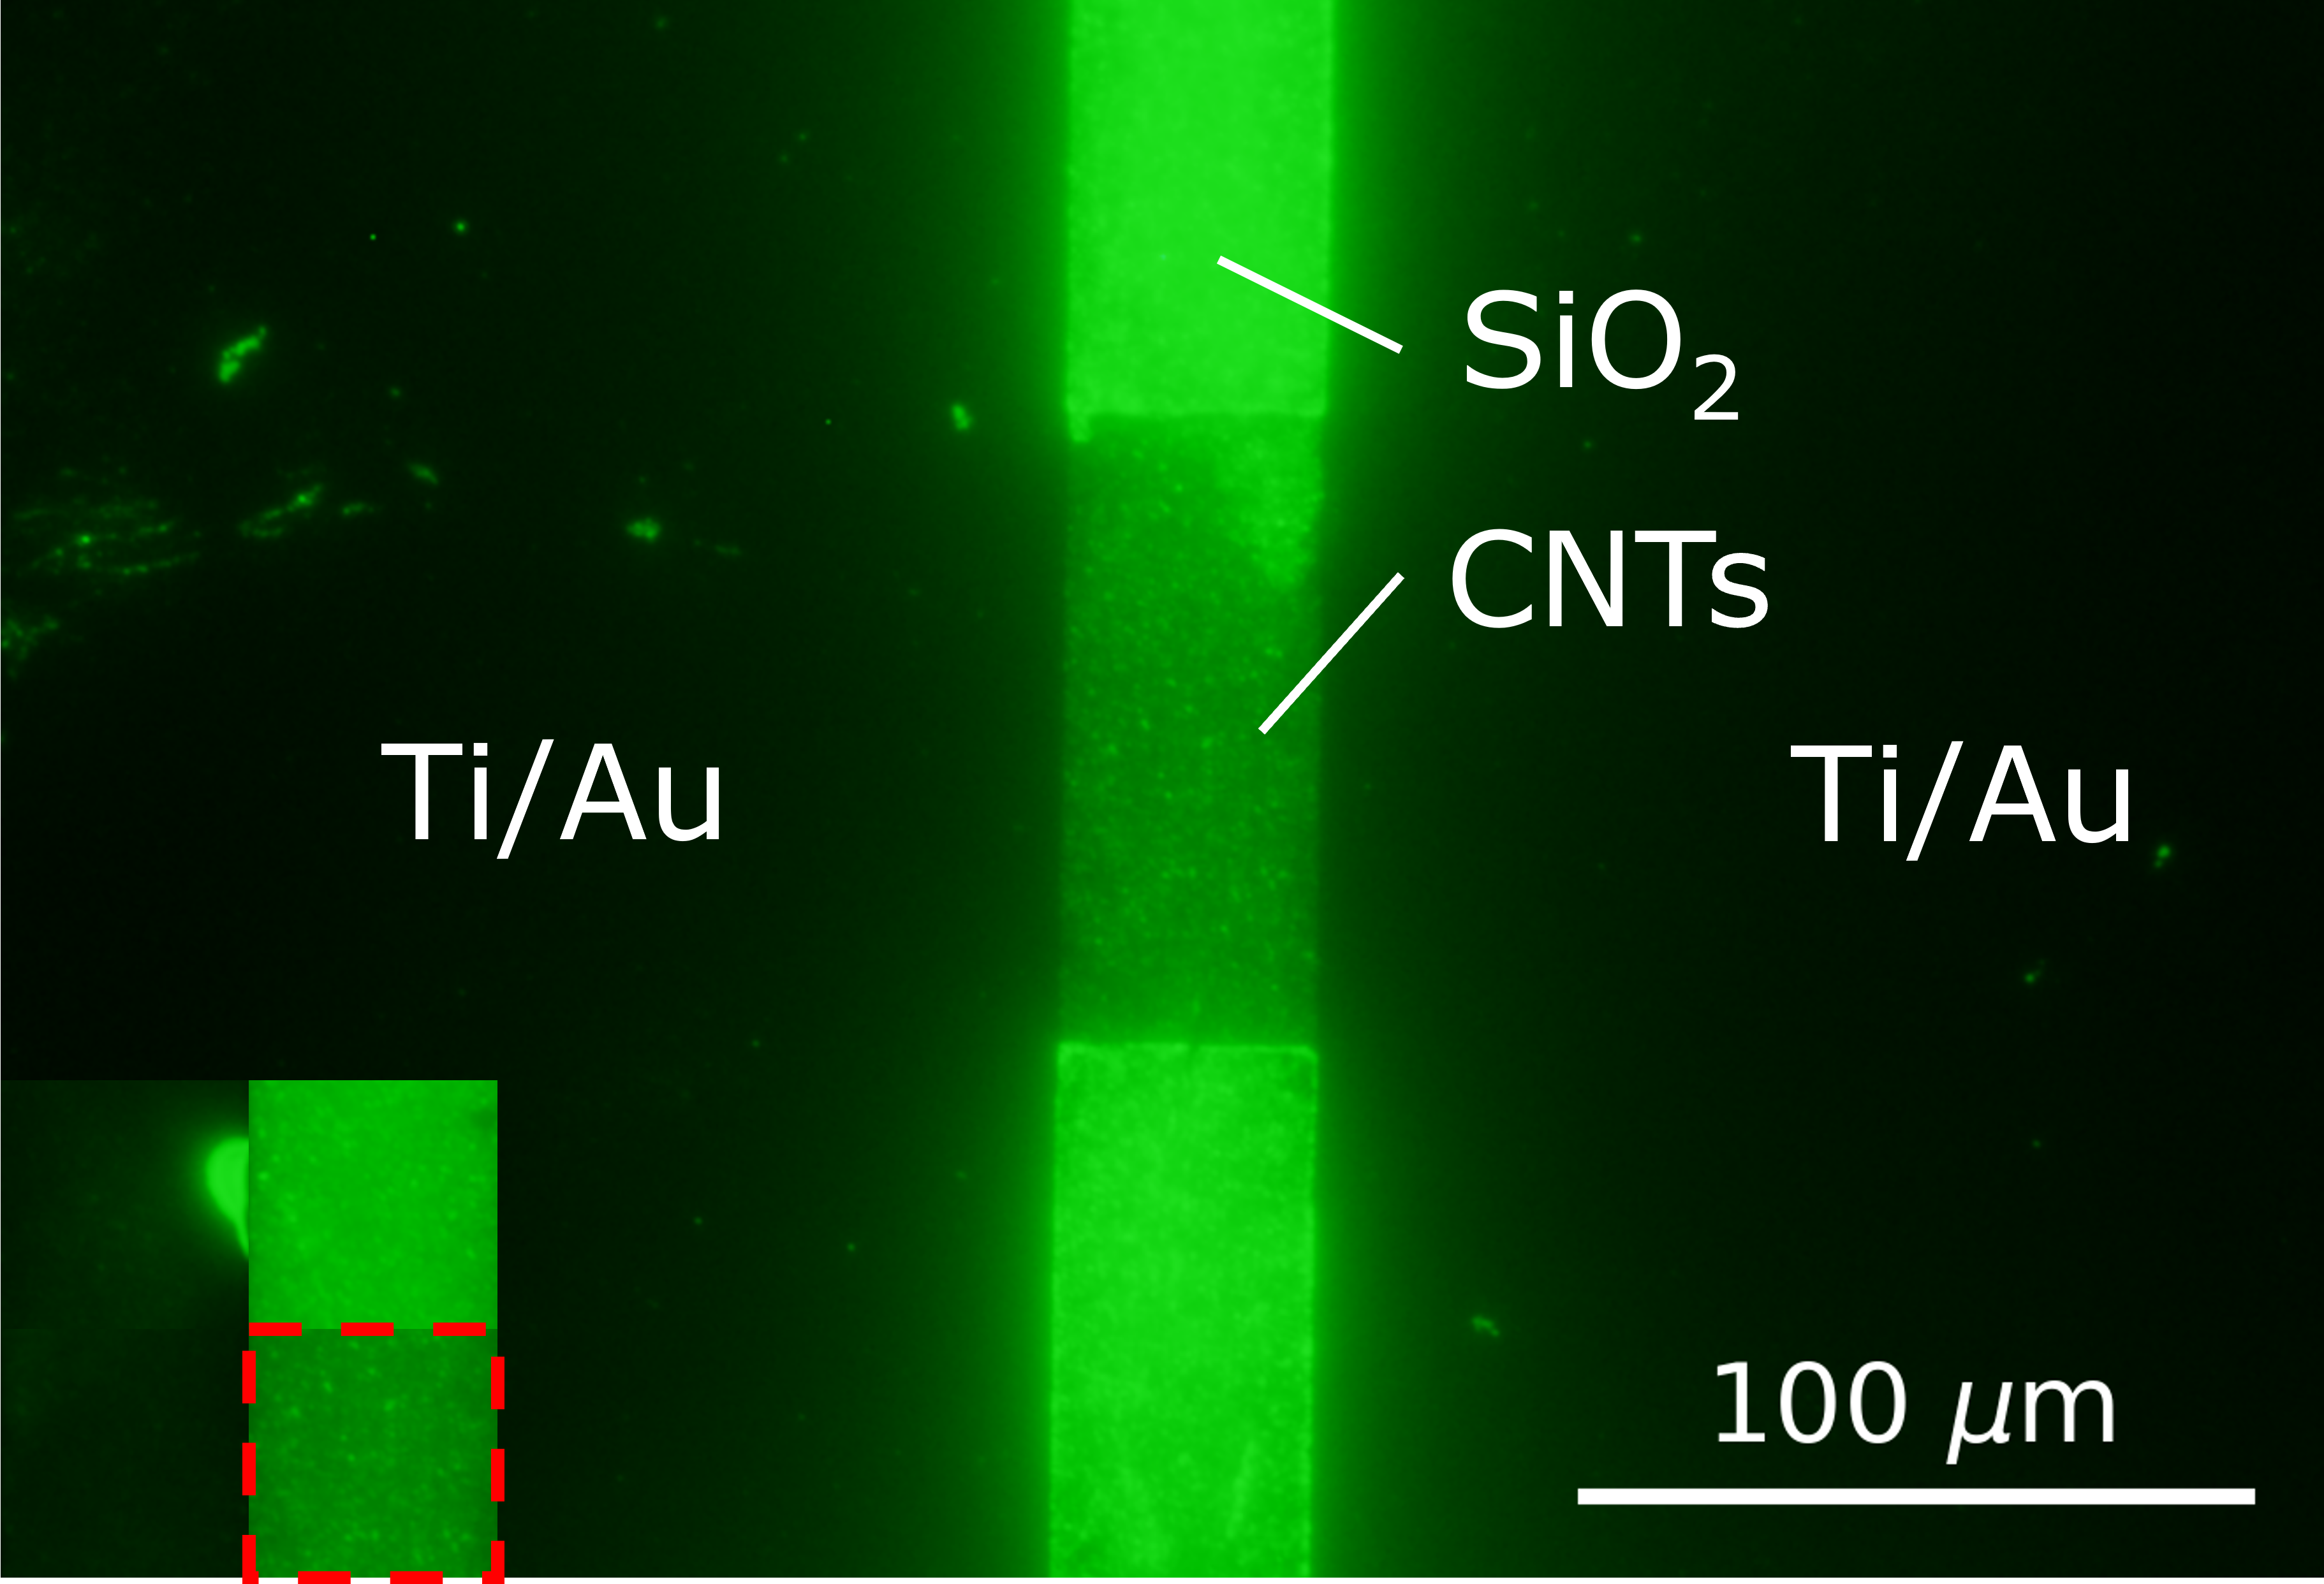
\includegraphics{figures/ch8/modified_GFPOR_PBASE_10sexposure_40X_mediumcontrast_ch2_231019.png}

}

}

\end{minipage}%
%
\begin{minipage}[t]{0.01\linewidth}

{\centering 

~

}

\end{minipage}%

\caption{\label{fig-PBASE-GFP-ORs}The fluorescence images on the left
side \(-\) (a), (c) and (e) \(-\) show unencapsulated carbon nanotube
network channels from a device incubated in GFP-OR nanodiscs. The
rectangular dark regions to the left and right of each image are the
gold electrodes. The fluorescence images on the right \(-\) (b), (d) and
(f) \(-\) show the channels of a similar device after successive PBASE
and GFP-OR nanodisc incubation. Images (a) and (c) are both of the same
channel on the first device, and images (b) and (d) are of the same
channel on the second, but (c) and (d) were taken using a greater
magnification. The insets in (c)-(f) compare the central channel region
of (c)-(f) more directly. All images were taken with the same microscope
settings (GFP filter and 10 s exposure time), taken in quick succession,
directly after functionalisation in a dark room.}

\end{figure}

Fluorescence microscopy was also used to confirm the presence of
GFP-tagged odorant receptors on the carbon nanotube network. A device
was functionalised using nanodiscs with odorant receptors attached to
\emph{Aequorea Victoria} green fluorescent protein (GFP) using the
process described earlier. When these nanodiscs were used, the
functionalisation was performed in darkness, with the odorant receptor
nanodisc vial transported under an opaque cover to protect it from light
(batch number ND-GFP-OR43b-0002, prepared 12 months earlier). After
functionalisation, devices were briefly rinsed with DI water and
nitrogen dried to remove dried-down salt residue left by the 1XPBS. A
control device was also prepared without the use of PBASE, skipping
steps 3 and 4 in the functionalisation process. Fluorescence images of
the GFP-OR functionalised and control devices are shown in
Figure~\ref{fig-PBASE-GFP-ORs}. Note that fluorescence microscope images
were taken immediately after functionalisation; devices were transported
to the fluorescence microscope room in a foil-wrapped container, and the
fluorescence microscope room was kept dark while images were taken.

The silicon dioxide regions in each image appear bright under the GFP
filter, indicating non-specific binding between the GFP-OR nanodiscs and
the silicon dioxide substrate. As this device has been annealed, UV
exposed and developed before functionalisation, the likelihood this
non-specific attachment is to residual photoresist is reduced
significantly (see \textbf{?@sec-photoresist-contamination}). The
SiO\(_2\) substrate also appears brighter in the images on the right of
Figure~\ref{fig-PBASE-GFP-ORs}, which are of the device initially
exposed to PBASE. The discussion in \textbf{?@sec-pyrene-interactions}
indicates that the pyrene moiety of PBASE non-specifically interacts
with the silicon dioxide substrate. Assuming no significant variation in
the fluorescence of GFP between nanodisc vials, the PBASE coating
appears have led to more nanodiscs attaching to the silicon dioxide,
giving rise to the brighter fluorescence of the silicon dioxide seen for
the PBASE-incubated device on the right of
Figure~\ref{fig-PBASE-GFP-ORs}.

A comparison of fluorescence in the channel region between images on the
left of Figure~\ref{fig-PBASE-GFP-ORs} (GFP-OR nanodiscs) and the images
on the right (GFP-OR nanodiscs and PBASE) is given by the inset in
Figure~\ref{fig-PBASE-GFP-ORs} (c)-(f). The inset demonstrates that the
channels not incubated in PBASE are significantly less bright than those
that had been incubated with PBASE. It appears that the presence of
GFP-OR nanodiscs in 1XPBS is limited on these channels. However, when
the carbon nanotubes are modified with PBASE, the GFP-OR nanodiscs are
able to attach to the channel, and so the channel shows up brightly
under the fluorescence microscope GFP filter. Importantly, since the GFP
is attached to odorant receptors rather than the nanodiscs themselves,
there must be odorant receptors present on the channel after
functionalisation; attachment to the channel is not limited to empty
nanodiscs. This trend was consistent across all conducting channels on
each of the two devices. As far as I know, this is the first time
fluorescence has been used to investigate the attachment of odorant
receptor nanodiscs to a carbon nanotube network.

\hypertarget{sec-EtHex-aqueous-sensing}{%
\subsection{Aqueous Sensing of Ethyl
Hexanoate}\label{sec-EtHex-aqueous-sensing}}

The procedure used for biosensor detection of ethyl hexanoate in liquid
was the same as the procedure outlined in \textbf{?@sec-dummy-sensing},
except 0.5\% v/v DMSO was present in the buffer solution (to improve
ethyl hexanoate solubility) and dilutions of ethyl hexanoate in the same
0.5\% v/v DMSO 1XPBS buffer solution were added during the sensing
series. The 0.5\% v/v DMSO 1XPBS was prepared by adding 5 µL of DMSO to
995 µL 1XPBS before device characterisation. The dilutions of ethyl
hexanoate were prepared with the same 1XPBS at the same time, where 5 µL
of 200 fM, 200 pM, 200 nM and 200 µM ethyl hexanoate in DMSO were placed
into four individual vials containing 995 µL 1XPBS each, giving 1mL
vials of 1 fM, 1 pM, 1 nM and 1 µM ethyl hexanoate in 0.5\% v/v DMSO
1XPBS. The ethyl hexanoate in DMSO dilutions were prepared beforehand as
a 1:10 dilution series in DMSO using 200 mM stock solution, where
dilutions ranged from 20 mM to 200 fM. Sampling measurements were taken
using the B1500A semiconductor device analyser, with the transfer
measurement in Figure~\ref{fig-OR22a-TX-comparison} (b) taken directly
before sensing. The full control series plus sensing sequence is shown
in Figure~\ref{fig-EtHex-aqueous-sensing}. Gate current remained
negligible across the entire sensing procedure.

\begin{figure}

{\centering 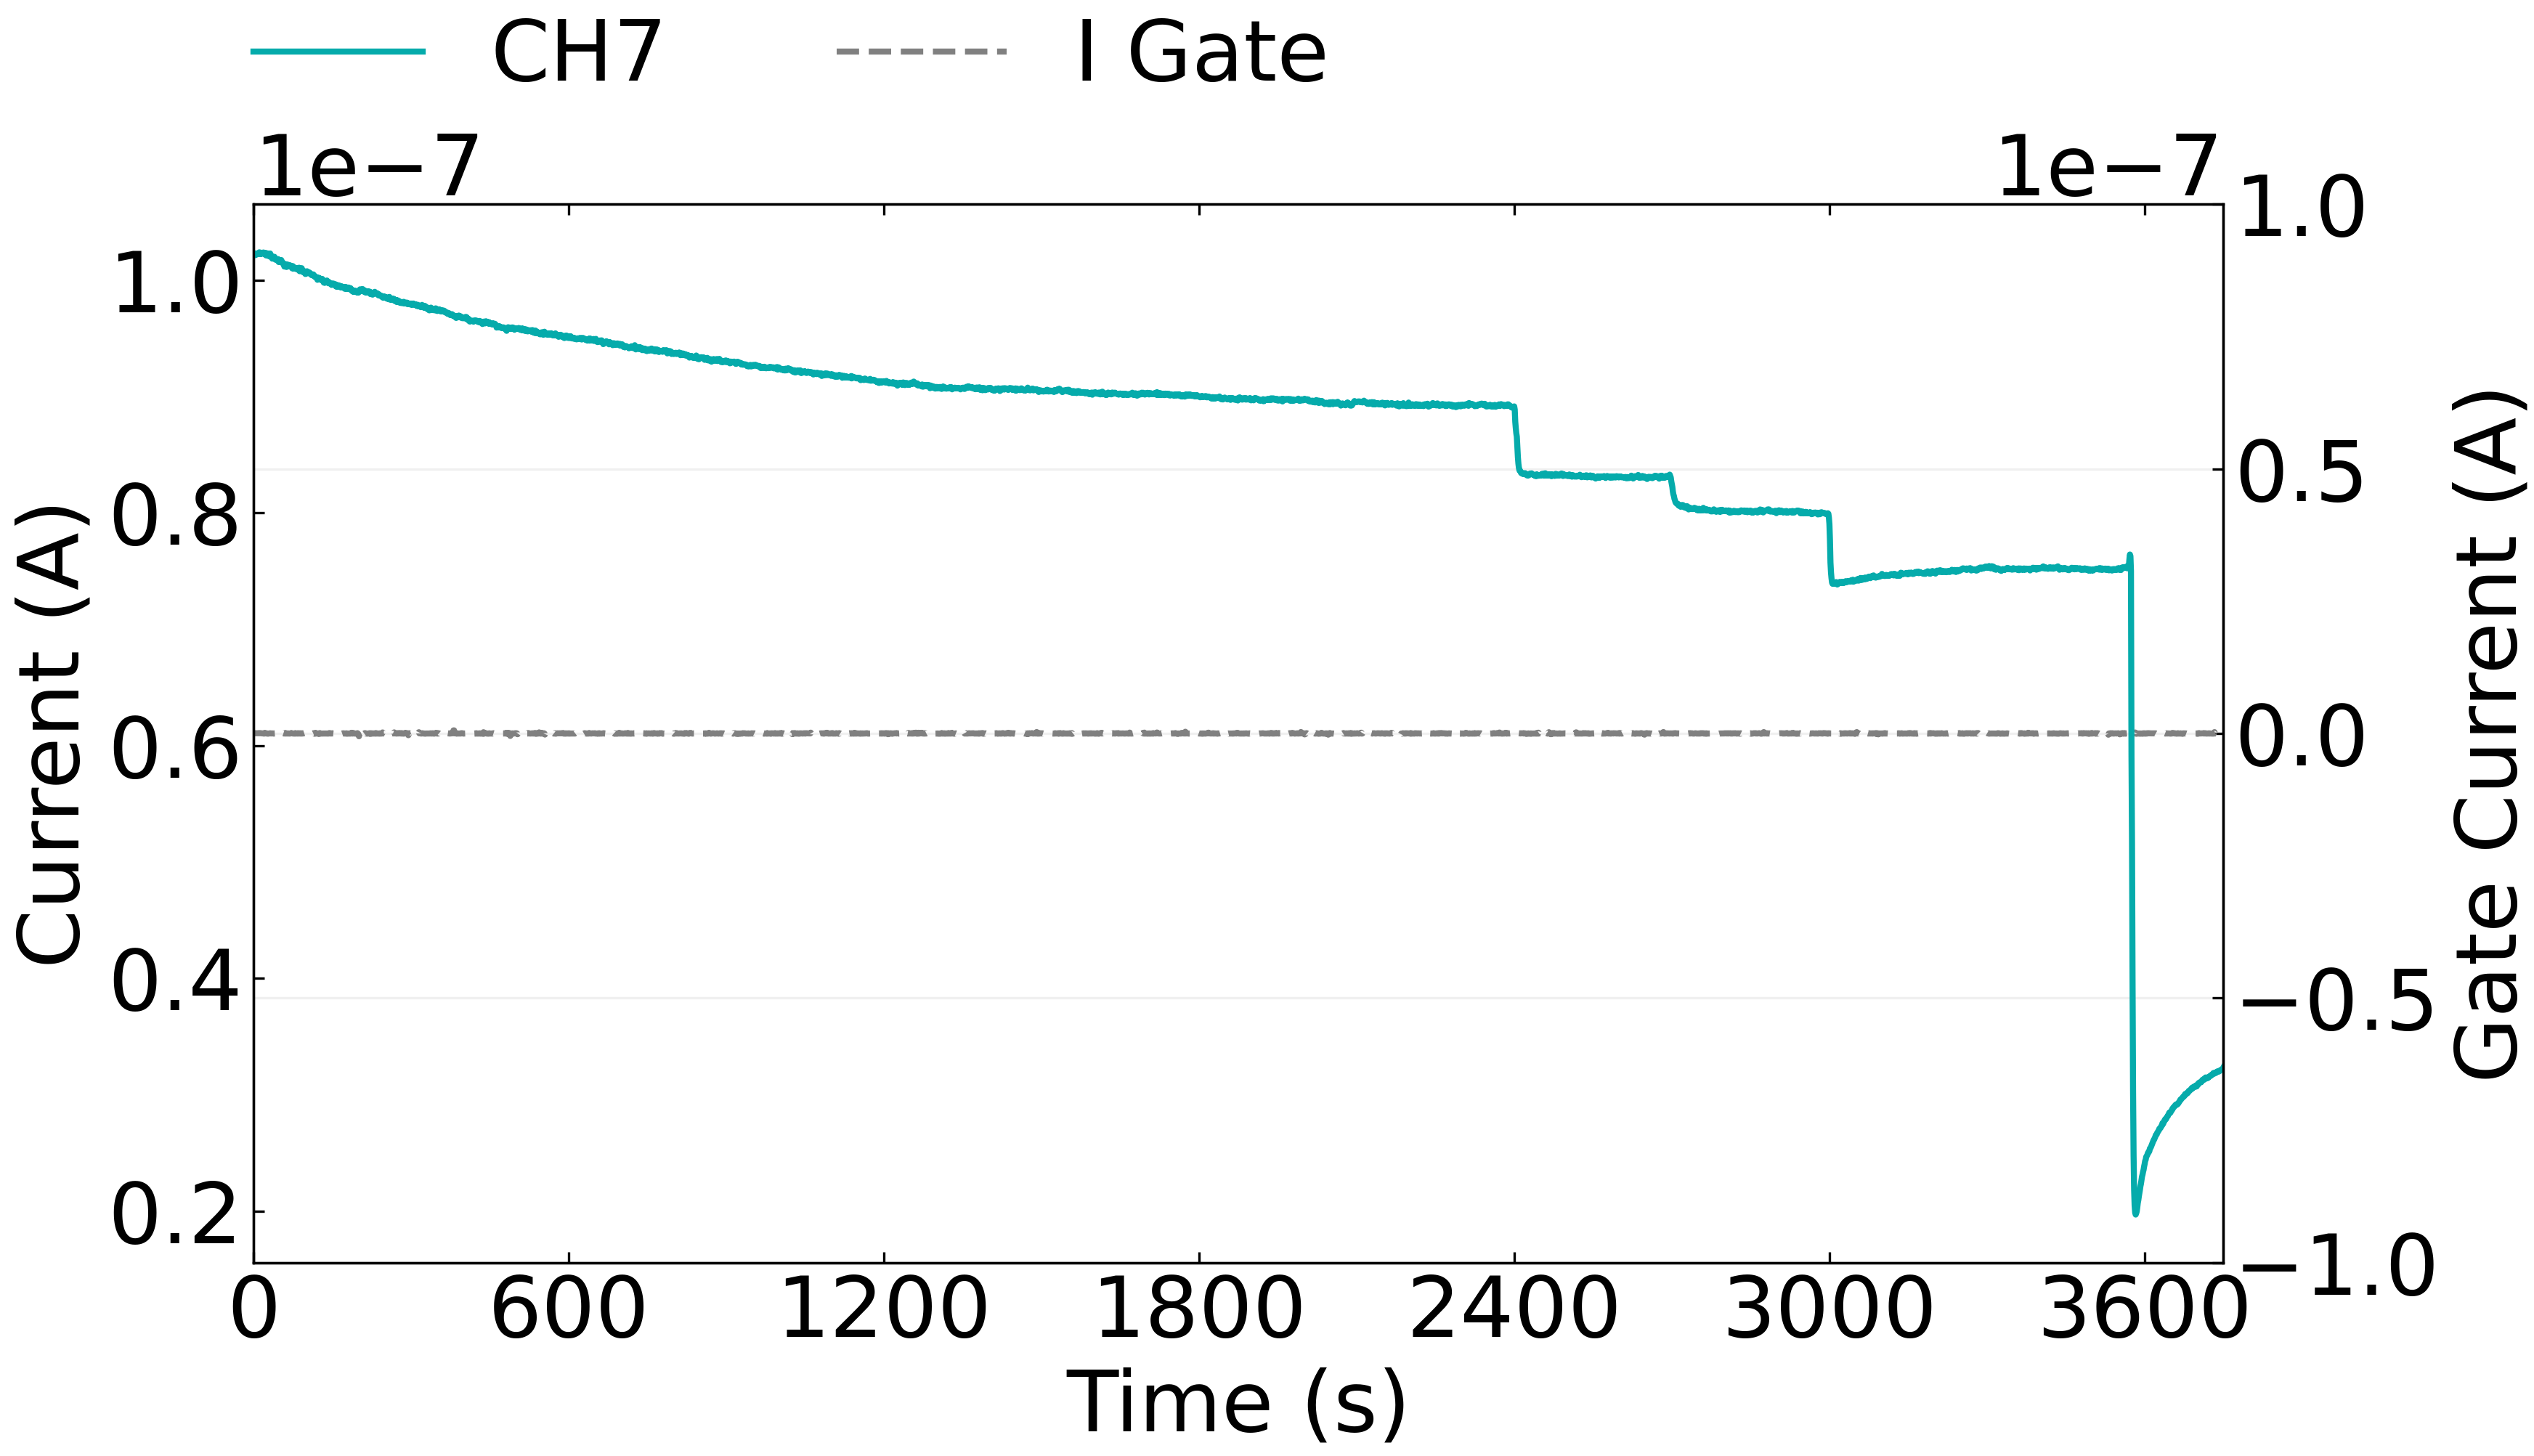
\includegraphics[width=0.7\textwidth,height=\textheight]{figures/ch8/Q1C6.png}

}

\caption{\label{fig-EtHex-aqueous-sensing}The control series (before
1800 s) and ethyl hexanoate sensing series (after 1800 s) of the
OR22a-functionalised device channel. Source-drain current was set at
\(V_{ds}\) = 100 mV while gate current was set at \(V_g\) = 0 V. No
responses to 0.5\% v/v DMSO 1XPBS were seen during the control series,
while significant responses to additions of ethyl hexanoate diluted in
0.5\% v/v DMSO 1XPBS were seen at 2400 s, 2700 s, 3000 s and 3600 s.
Functionalisation and sensing was performed by Danica Fontein, School of
Chemical and Physical Sciences, Te Herenga Waka - Victoria University of
Wellington, using the methods developed in this thesis.}

\end{figure}

The control series for the sensing series is shown in
Figure~\ref{fig-OR22a-control-series} (a). No clear stepwise response is
seen to buffer additions or subtractions. The functionalised device
shows similar baseline drift behaviour to that of a pristine device,
with a period of short-term decay quickly yielding to a more long-lived
decay behaviour. A linear fit \(I = c_1t + c_2\) to the region
\(1200-1800\) s had a gradient of \(c_1 = -1.76\pm0.02\) pA/s. This
gradient is smaller than the range of values found for the linear fit
approximating the longer-term drift of a pristine device
(\textbf{?@sec-baseline-drift}), but of the same order of magnitude. The
linear fit was then subtracted from the control series and an
exponential fit \(I = I_0\exp(-t/\tau)\) was performed on the remaining
dataset, as shown in Figure~\ref{fig-OR22a-control-series} (b). A value
of \(590 \pm 3\) s was found for the exponential time constant, similar
to those found for the channels of the pristine device. This confirms
that the 1800 s control series is sufficient to avoid the presence of
short-term decay during sensing.

\begin{figure}

\begin{minipage}[t]{0.11\linewidth}

{\centering 

~

}

\end{minipage}%
%
\begin{minipage}[t]{0.03\linewidth}

{\centering 

\raisebox{-\height}{


\includegraphics{figures/(a).png}

}

}

\end{minipage}%
%
\begin{minipage}[t]{0.01\linewidth}

{\centering 

~

}

\end{minipage}%
%
\begin{minipage}[t]{0.70\linewidth}

{\centering 

\raisebox{-\height}{

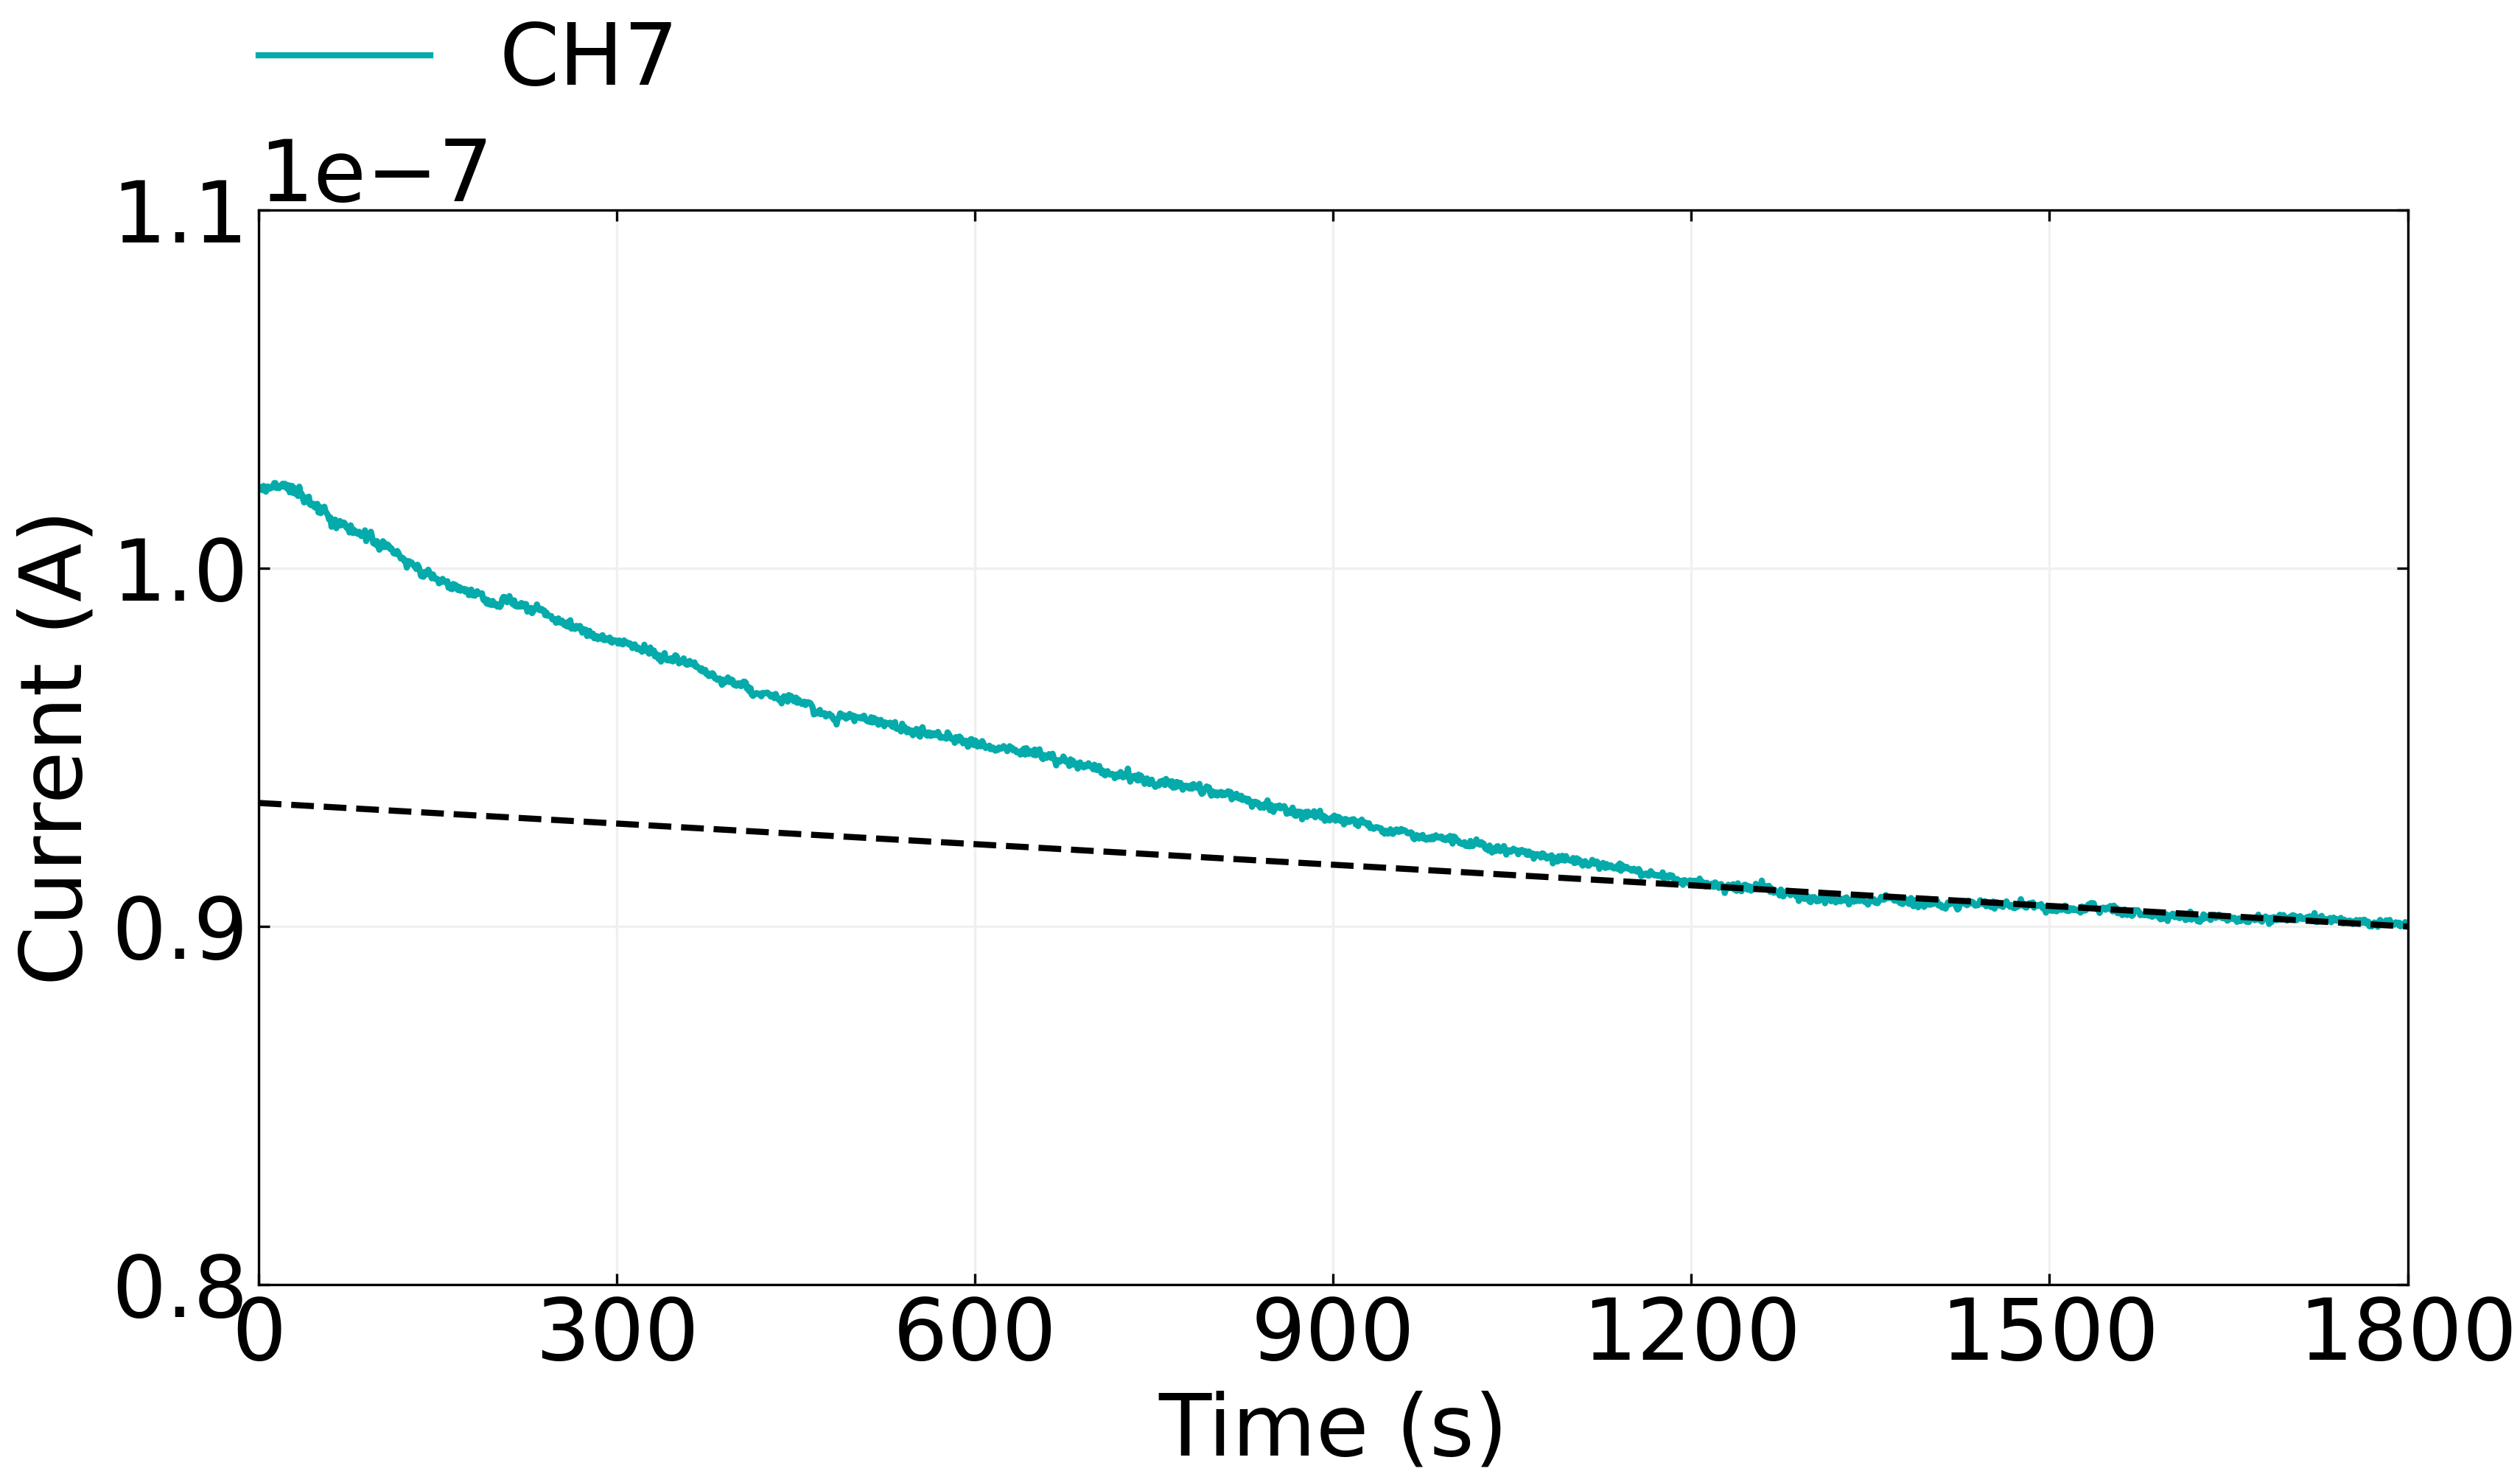
\includegraphics{figures/ch8/Q1C6_with_fitted_curves.png}

}

}

\end{minipage}%
%
\begin{minipage}[t]{0.15\linewidth}

{\centering 

~

}

\end{minipage}%
\newline
\begin{minipage}[t]{0.11\linewidth}

{\centering 

~

}

\end{minipage}%
%
\begin{minipage}[t]{0.03\linewidth}

{\centering 

\raisebox{-\height}{


\includegraphics{figures/(b).png}

}

}

\end{minipage}%
%
\begin{minipage}[t]{0.01\linewidth}

{\centering 

~

}

\end{minipage}%
%
\begin{minipage}[t]{0.70\linewidth}

{\centering 

\raisebox{-\height}{

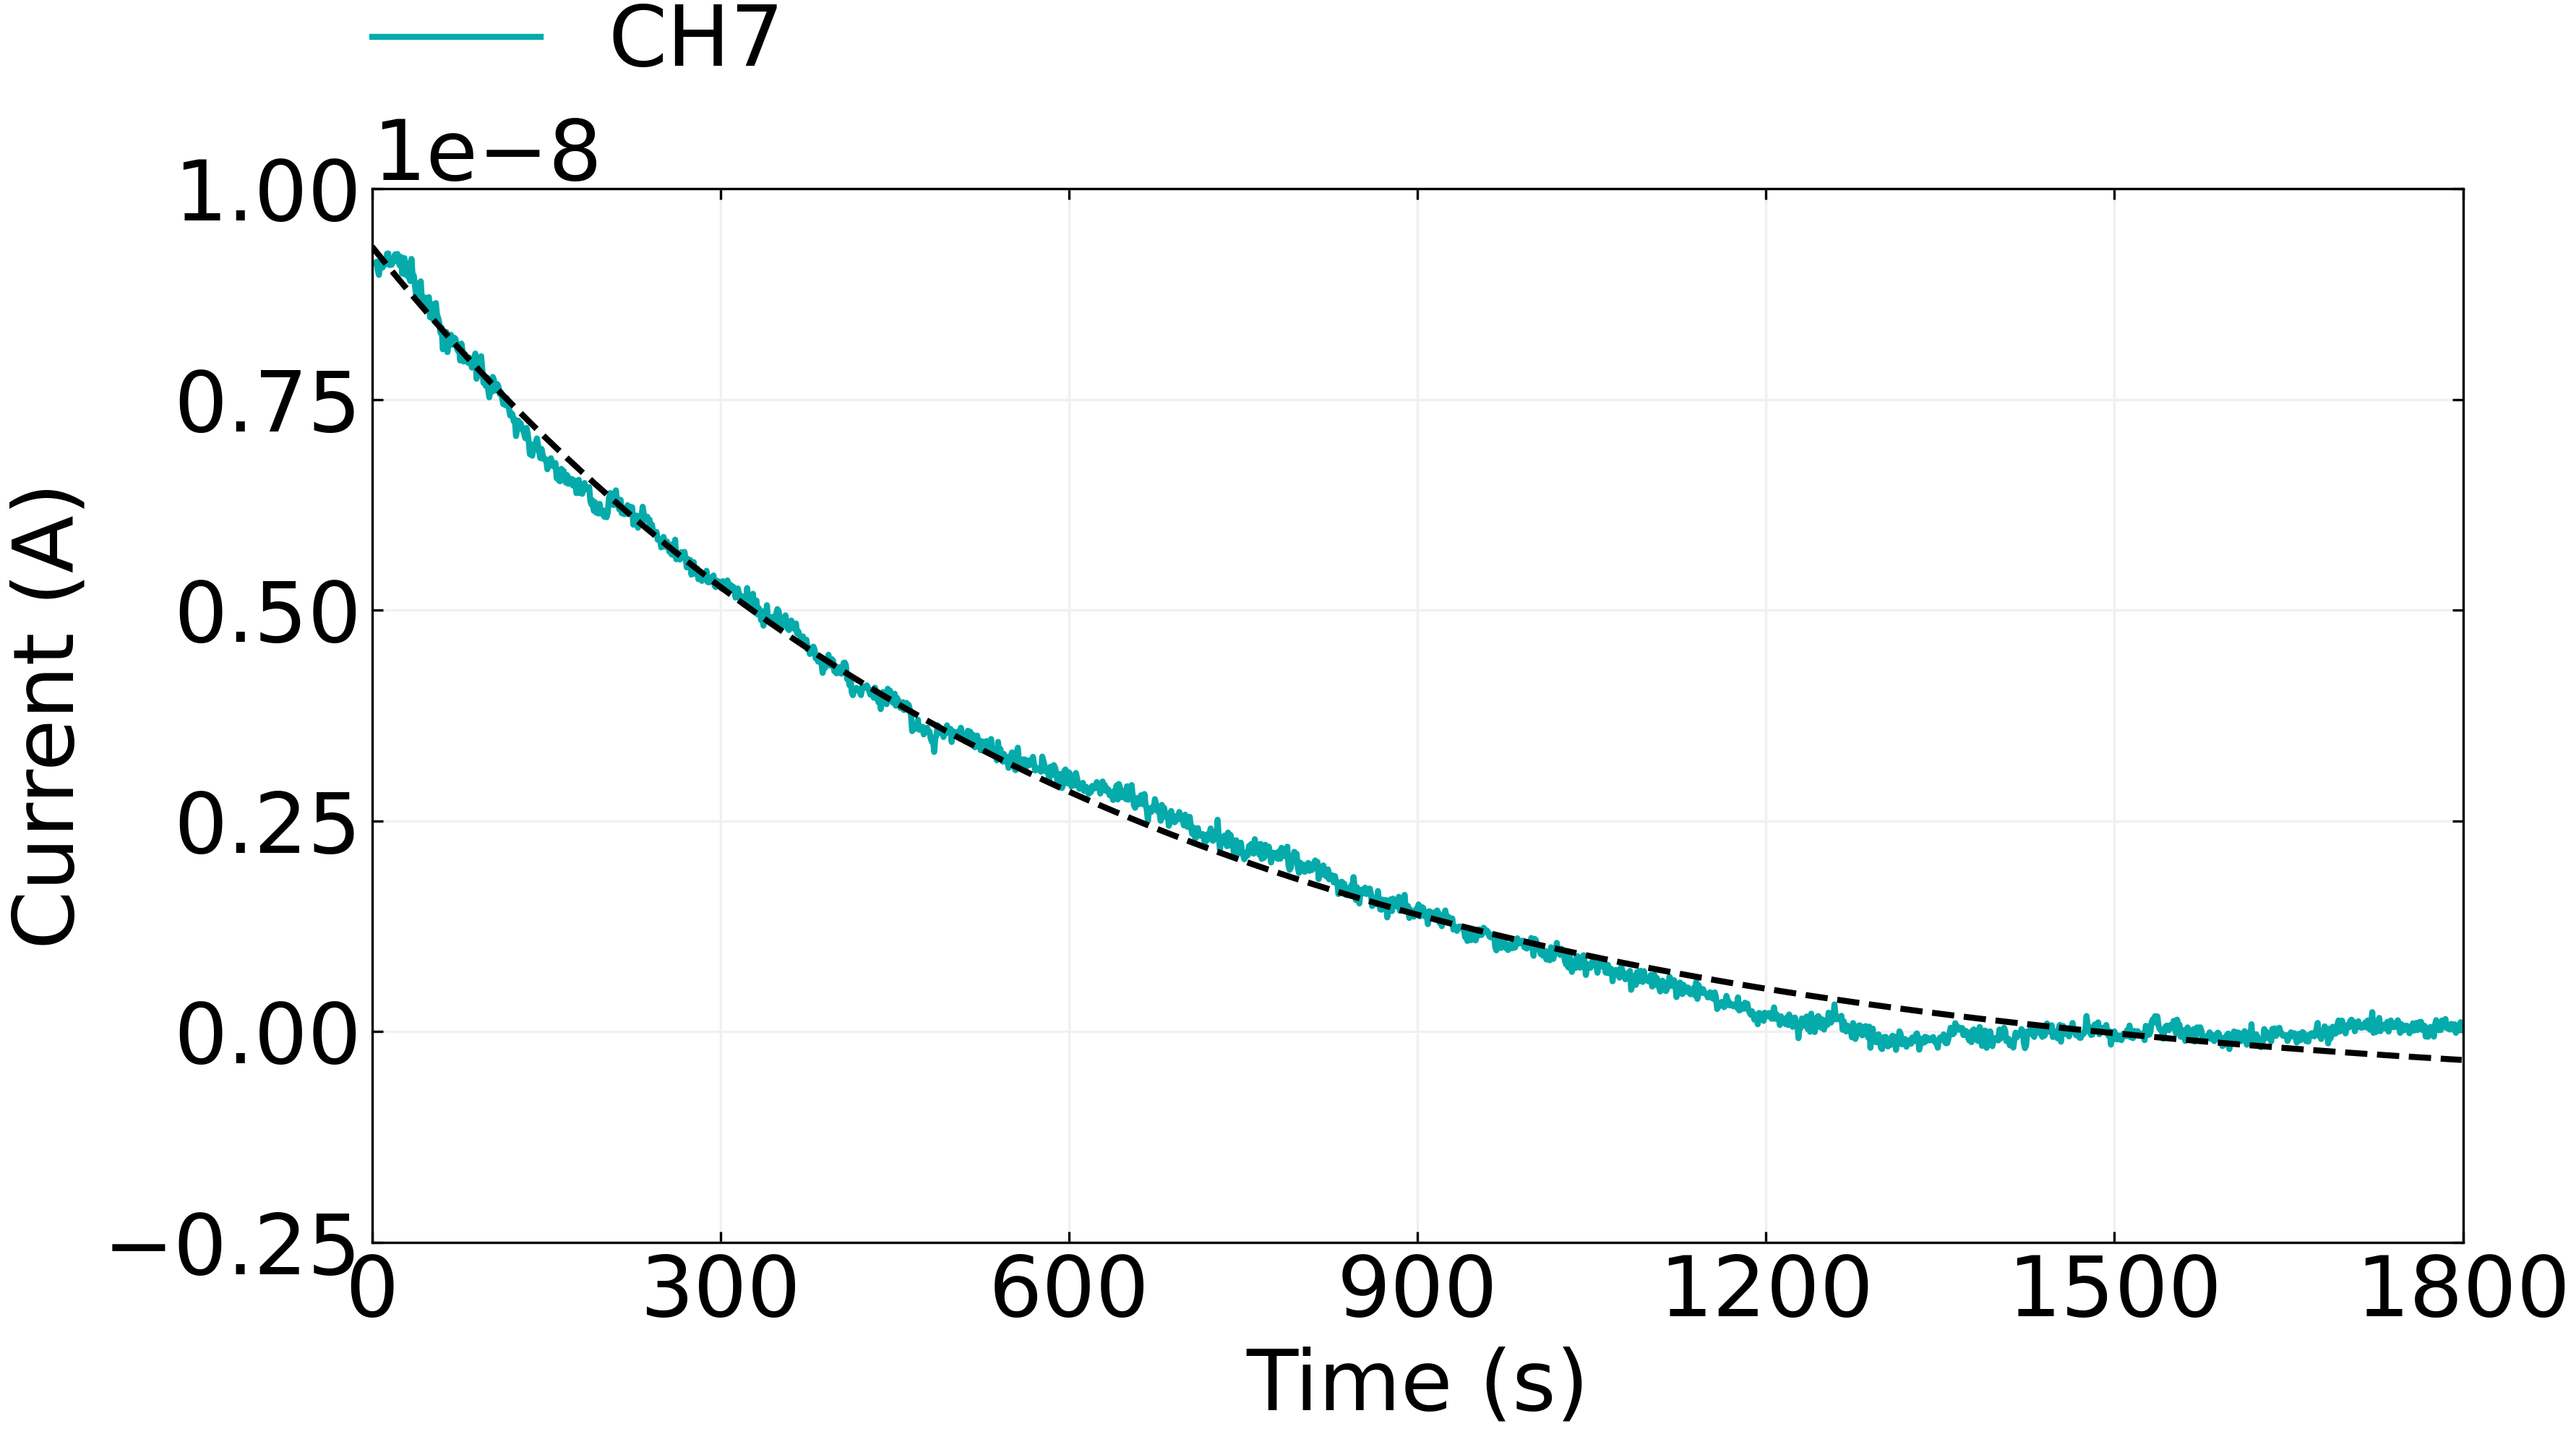
\includegraphics{figures/ch8/Q1C6_with_fitted_curves_exp.png}

}

}

\end{minipage}%
%
\begin{minipage}[t]{0.15\linewidth}

{\centering 

~

}

\end{minipage}%

\caption{\label{fig-OR22a-control-series}The control series for the
OR22a-functionalised device is shown in (a), alongside an extrapolated
linear fit to the control series from 1200 s onwards. The control series
with the linear approximation subtracted fitted to an exponential curve
is shown in (b).}

\end{figure}

It appears that the exponential fit overestimates current measurements
between 1100 s and 1500 s and underestimates measurements between 1500 s
and 1800 s. This deviation from the fit may result from the linear
approximation used to represent long-term baseline drift being weaker
for this channel than for those discussed previously in
\textbf{?@sec-dummy-sensing} and \textbf{?@sec-pristine-EtHex}. This
could result from the exponential terms for long-term baseline drift
having relatively short time constants, so \(t\ll\tau_i\) no longer
holds and higher order terms in the linear approximation are no longer
negligible. This observation may indicate a relationship exists between
device functionalisation and the long-lived device decay behaviour.
However, it may simply result from the natural variation between
randomly-deposited device channels. Further work may be required to
confirm the existence of such a relationship, though this work is
outside the scope of this thesis.

\begin{figure}

\begin{minipage}[t]{0.11\linewidth}

{\centering 

~

}

\end{minipage}%
%
\begin{minipage}[t]{0.03\linewidth}

{\centering 

\raisebox{-\height}{


\includegraphics{figures/(a).png}

}

}

\end{minipage}%
%
\begin{minipage}[t]{0.01\linewidth}

{\centering 

~

}

\end{minipage}%
%
\begin{minipage}[t]{0.70\linewidth}

{\centering 

\raisebox{-\height}{

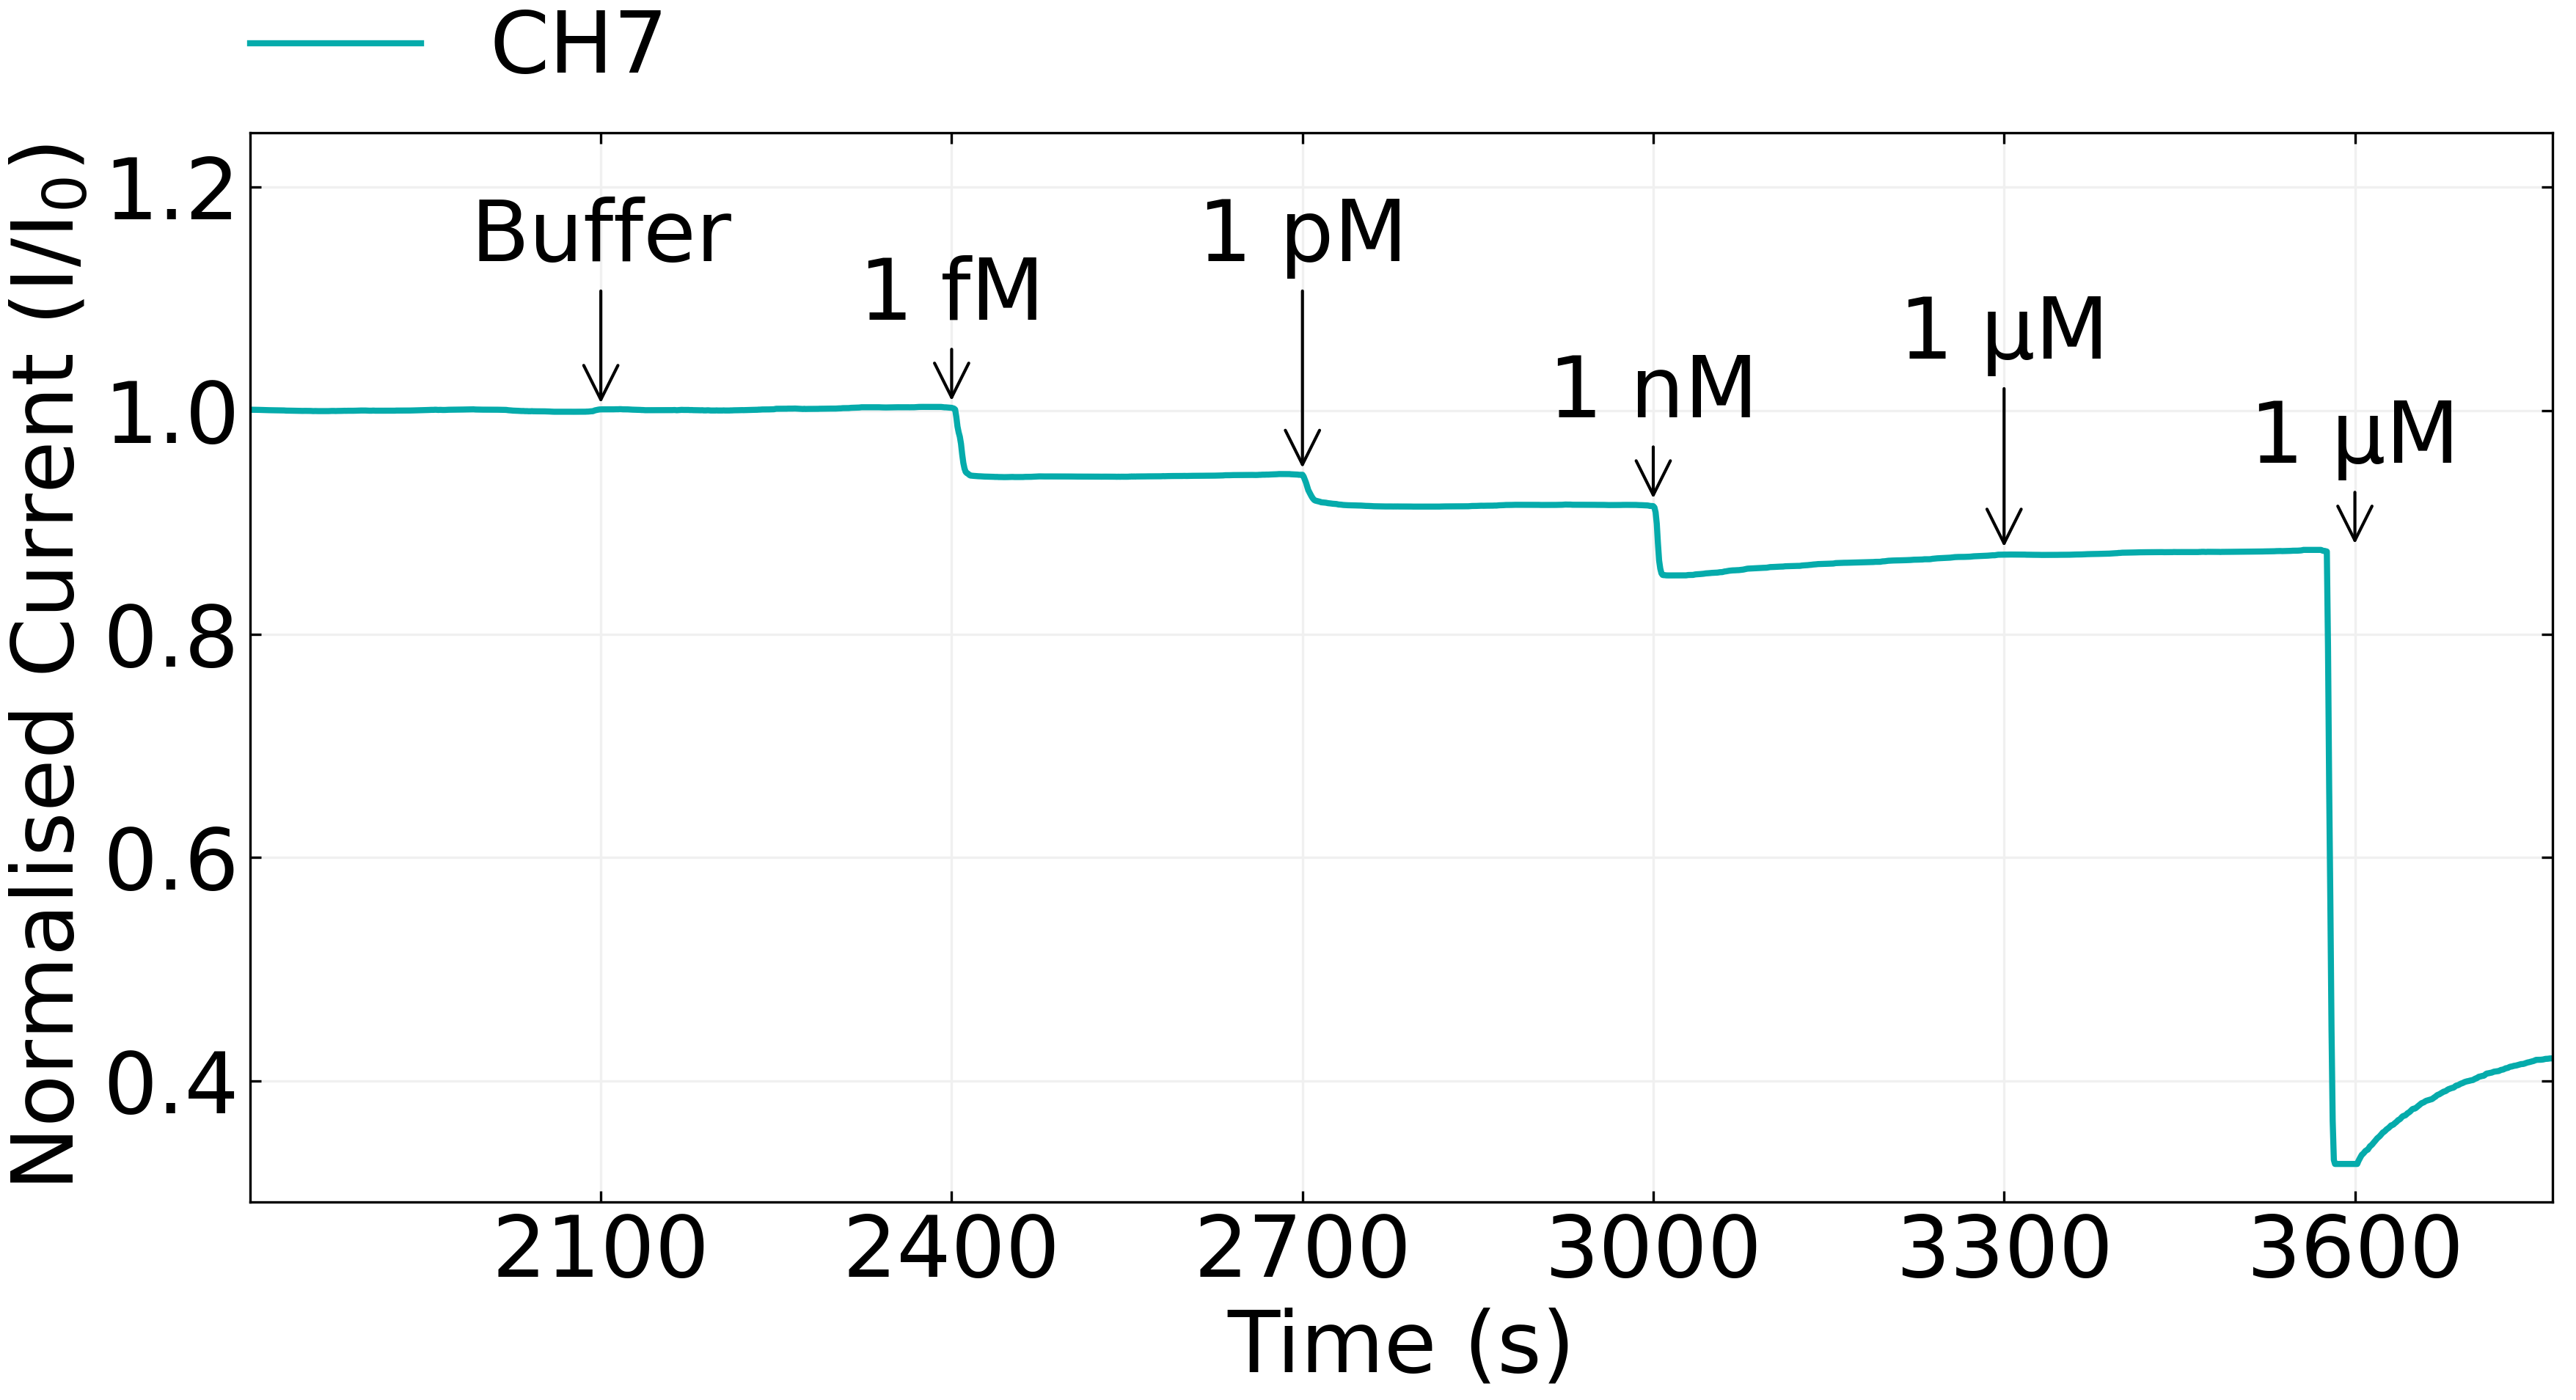
\includegraphics{figures/ch8/Q1C6_filtered_detrend_trunc_arrows_normalised.png}

}

}

\end{minipage}%
%
\begin{minipage}[t]{0.15\linewidth}

{\centering 

~

}

\end{minipage}%
\newline
\begin{minipage}[t]{0.11\linewidth}

{\centering 

~

}

\end{minipage}%
%
\begin{minipage}[t]{0.03\linewidth}

{\centering 

\raisebox{-\height}{


\includegraphics{figures/(b).png}

}

}

\end{minipage}%
%
\begin{minipage}[t]{0.01\linewidth}

{\centering 

~

}

\end{minipage}%
%
\begin{minipage}[t]{0.70\linewidth}

{\centering 

\raisebox{-\height}{

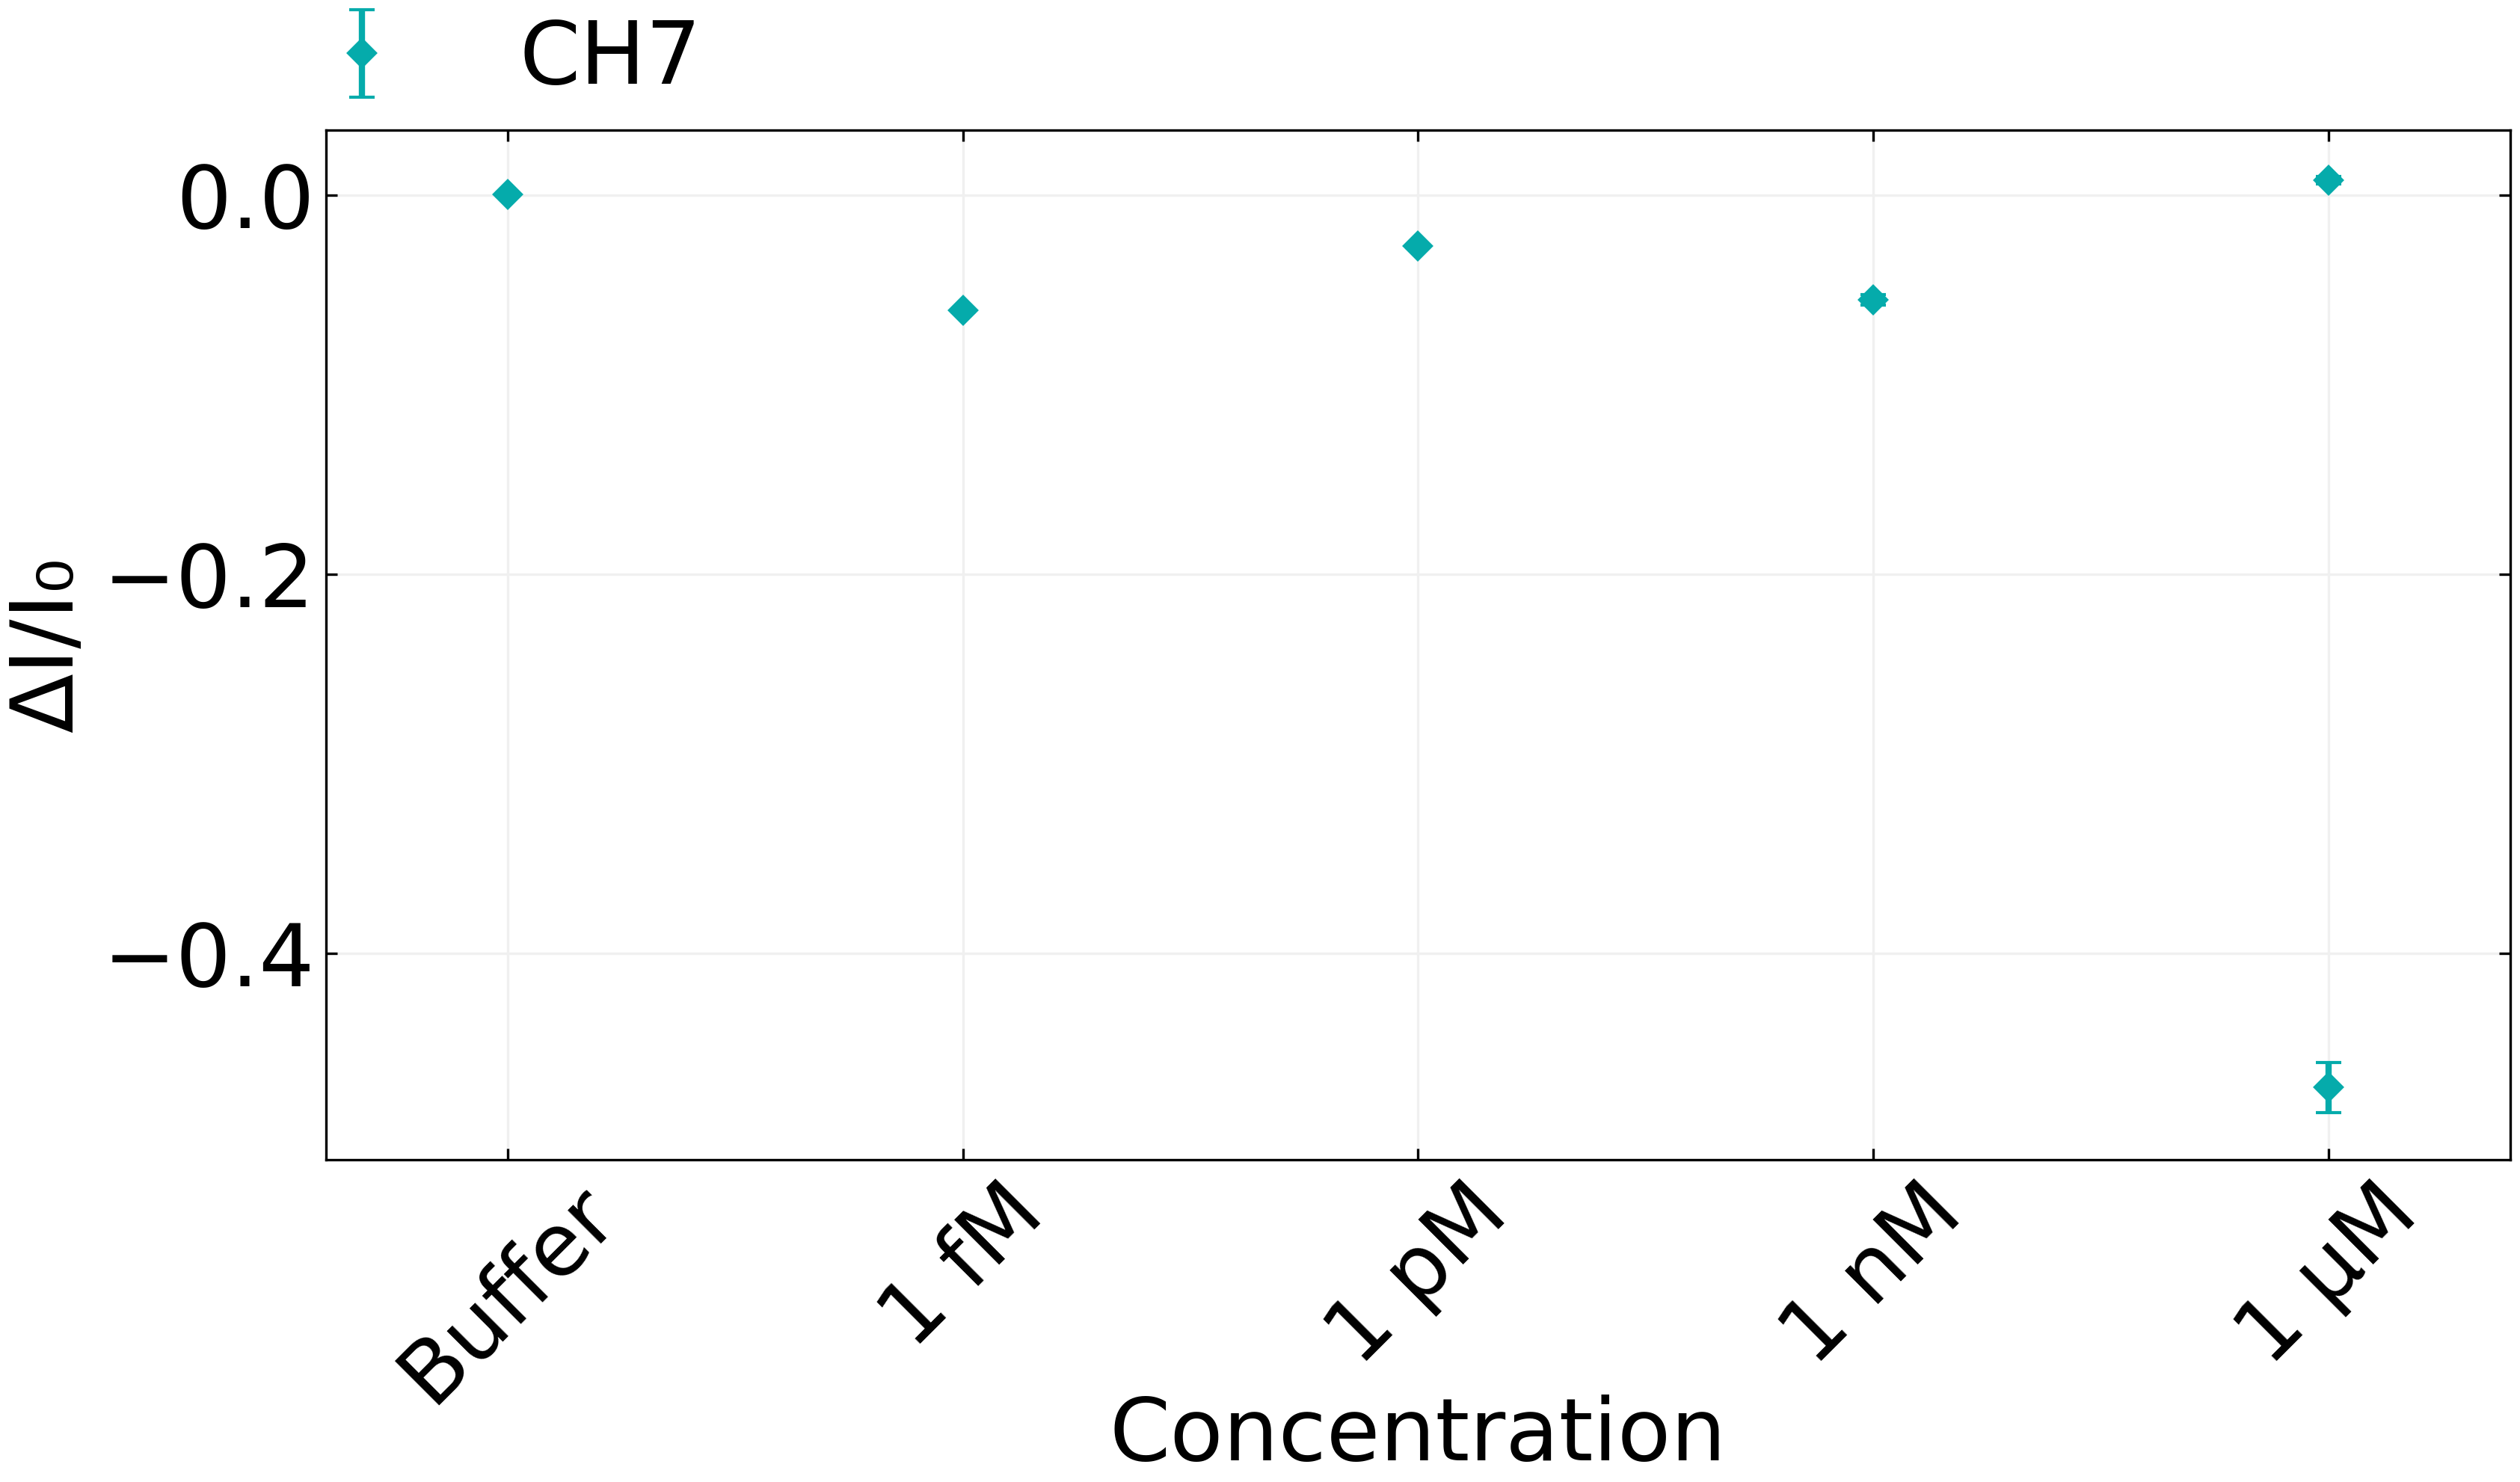
\includegraphics{figures/ch8/Q1C6_mean_simple_difference_before_and_after_step_filtered_concentrations.png}

}

}

\end{minipage}%
%
\begin{minipage}[t]{0.15\linewidth}

{\centering 

~

}

\end{minipage}%

\caption{\label{fig-OR22a-sensing-series}The normalised sensing series
for the OR22a-functionalised device is shown in (a). The current data
has been despiked, with baseline drift removed and a moving median
filter applied. The concentration of each 20 µL addition is indicated
above the time of addition. The signal data corresponding to the mean
difference in current before and after each addition is shown in (b).}

\end{figure}

Figure~\ref{fig-OR22a-sensing-series} (a) shows the cleaned and filtered
ethyl hexanoate sensing data from the OR22a-functionalised device from
1800 s onwards. The concentration of each 20 µL addition is indicated
above the corresponding addition time. The source-drain current across
the channel decreased rapidly with each addition of ethyl hexanoate in
0.5\% v/v DMSO 1XPBS solution. This current decrease appears
irreversible, as the current stabilises after each addition at a lower
current level than prior to the addition. This behaviour appears to be a
response by OR22a to its positive ligand ethyl hexanoate, similar to the
response by OR22a to methyl hexanoate seen by Murugathas \emph{et al.}.
The ORCO coreceptor was not required to be present for responses to be
seen. The device showed responses to ethyl hexanoate over a wide range
of concentrations, beginning with a \(\sim 6\)\% response to 1 fM EtHex
in 0.5\% v/v DMSO 1XPBS, while showing no response to any 0.5\% v/v DMSO
1XPBS buffer addition. Interestingly, as seen in
Figure~\ref{fig-OR22a-sensing-series} (b), no clear dose-dependent
response was observed. The behaviour seen may be explained by a
decreased sensitivity to subsequent additions seen by seen by Murugathas
\emph{et al.} \autocite{Murugathas2019b} competing with the logarithmic
increases in the concentration around the channel.

\hypertarget{sec-variability}{%
\section{Addressing Biosensor Variability}\label{sec-variability}}

\hypertarget{sec-variability-biosensor}{%
\subsection{Variability in Biosensor
Behaviour}\label{sec-variability-biosensor}}

\begin{figure}

\begin{minipage}[t]{0.11\linewidth}

{\centering 

~

}

\end{minipage}%
%
\begin{minipage}[t]{0.03\linewidth}

{\centering 

\raisebox{-\height}{


\includegraphics{figures/(a).png}

}

}

\end{minipage}%
%
\begin{minipage}[t]{0.01\linewidth}

{\centering 

~

}

\end{minipage}%
%
\begin{minipage}[t]{0.70\linewidth}

{\centering 

\raisebox{-\height}{

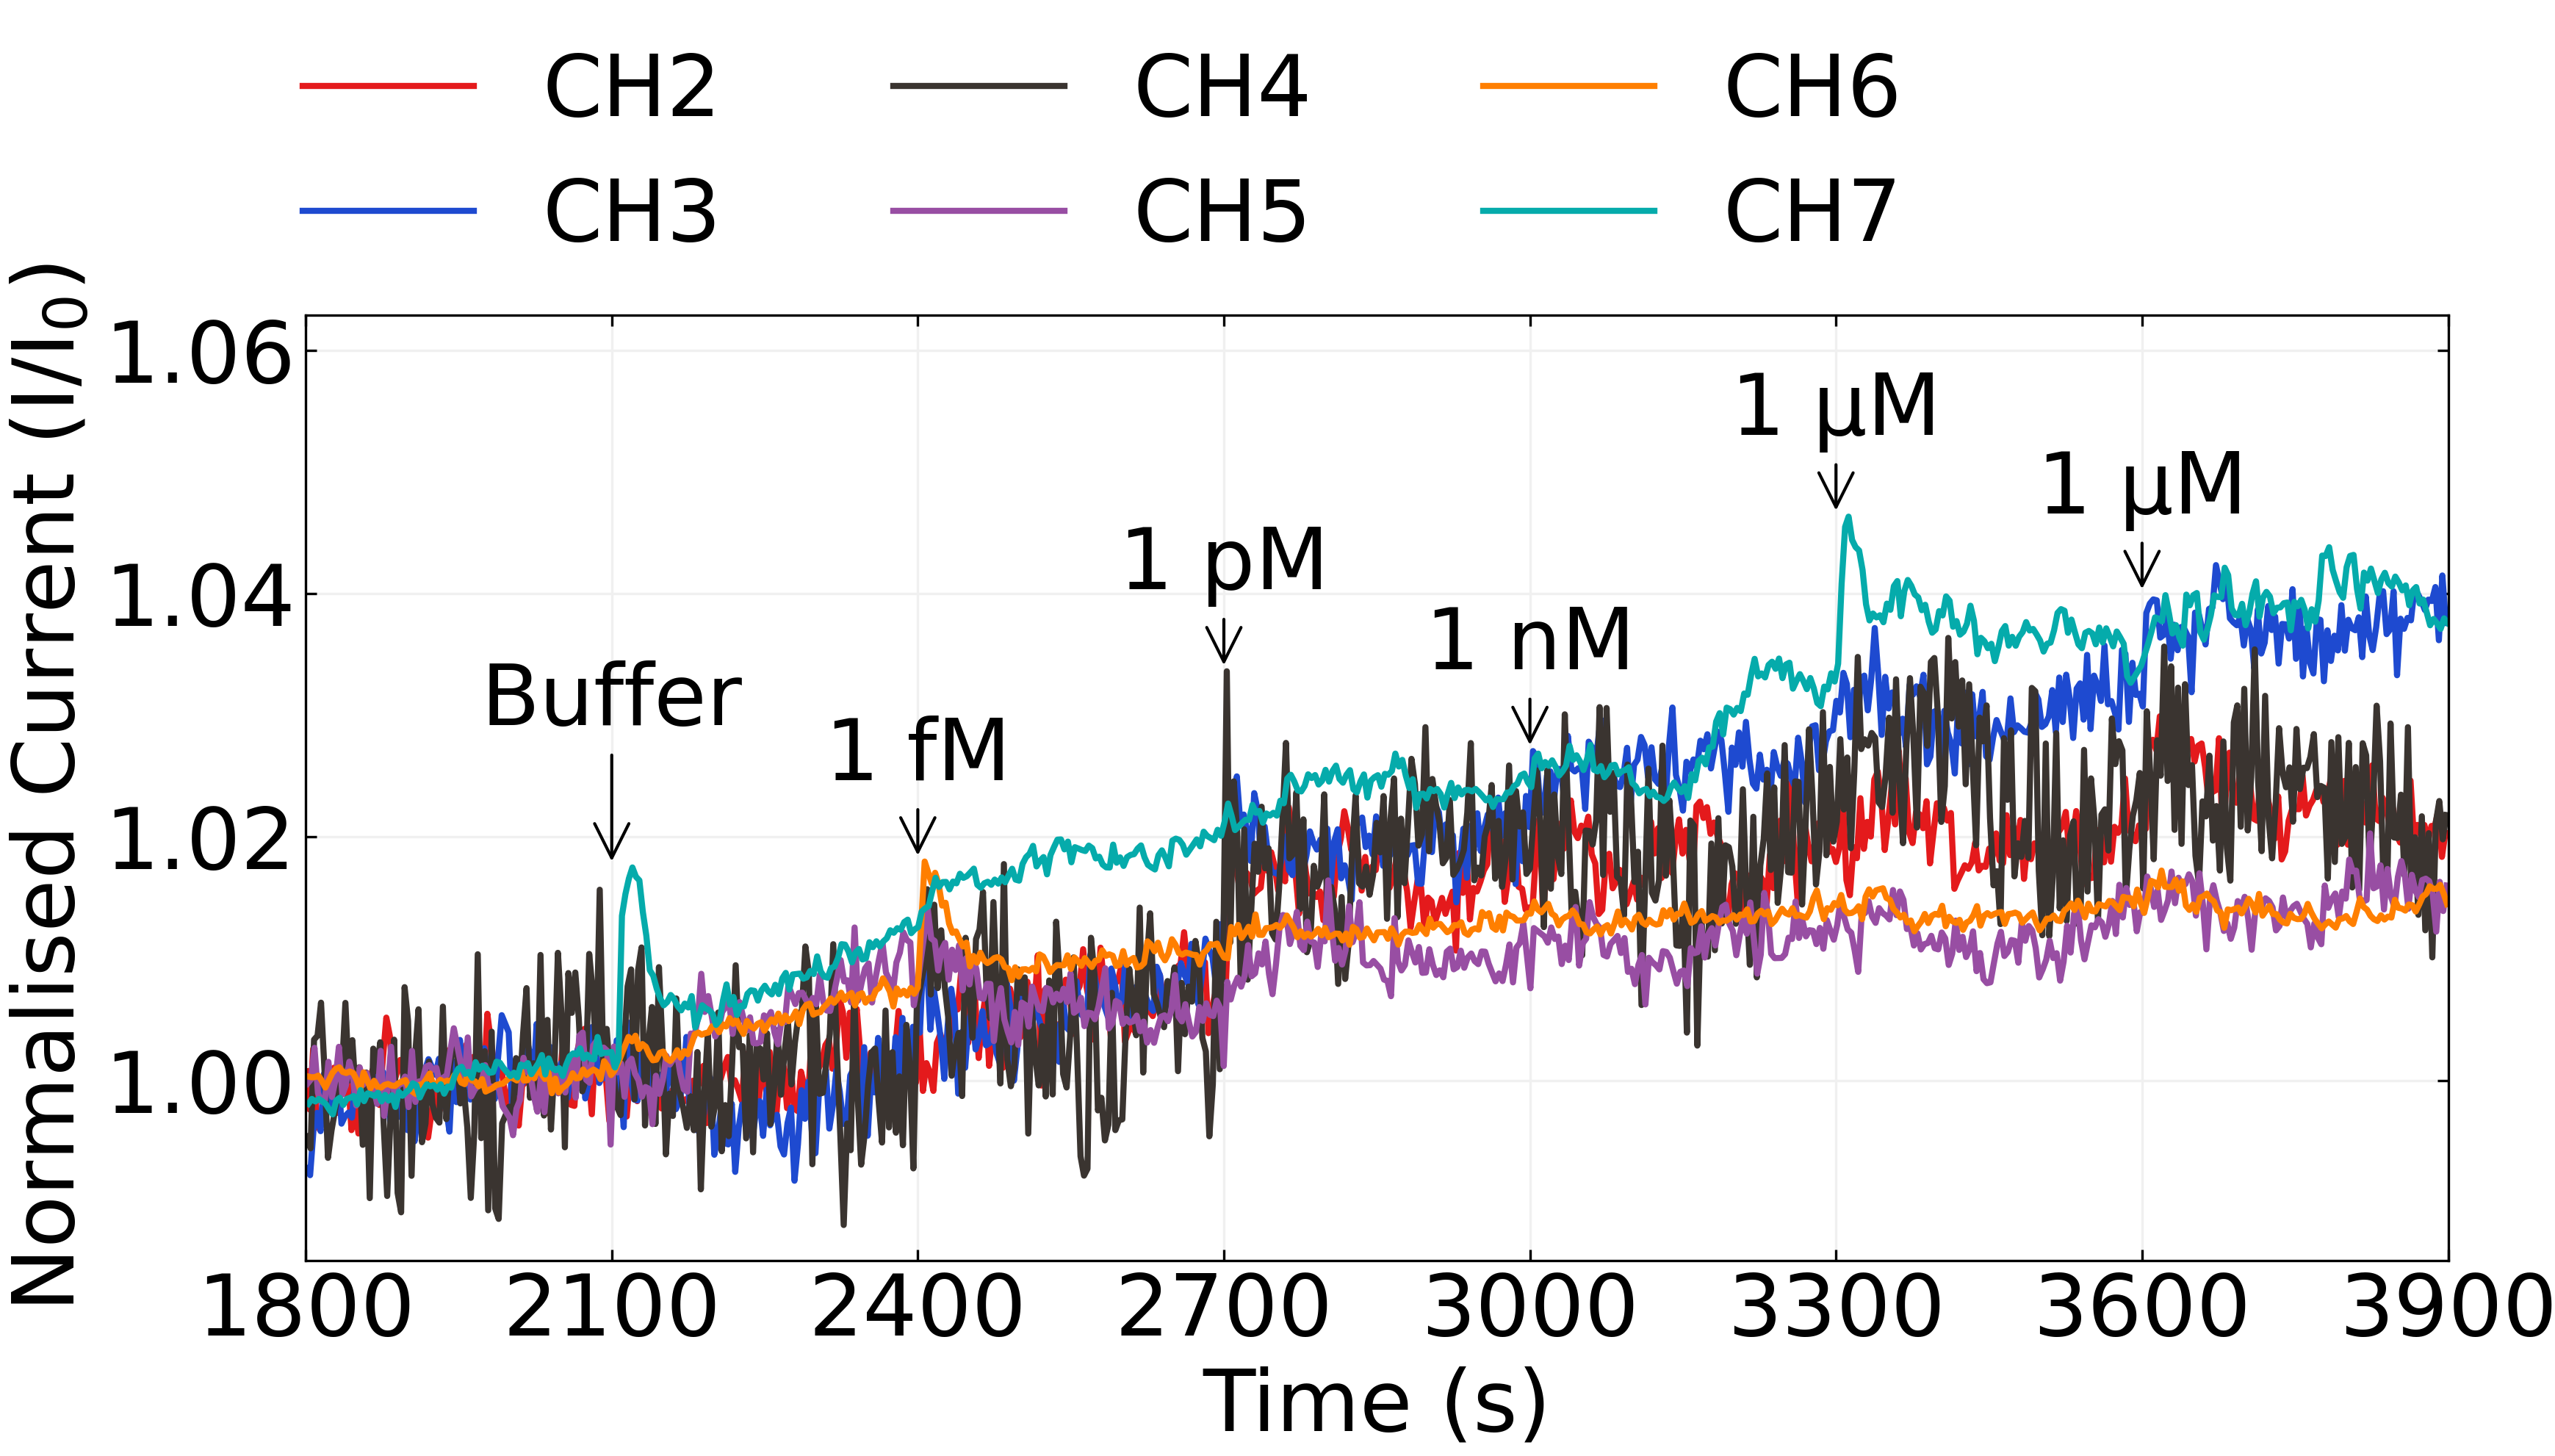
\includegraphics{figures/ch8/Q4C4_OR22a_Functionalised_2ndTimeSensingRun_48hrFridge_21_detrend_trunc_arrows_normalised.png}

}

}

\end{minipage}%
%
\begin{minipage}[t]{0.15\linewidth}

{\centering 

~

}

\end{minipage}%
\newline
\begin{minipage}[t]{0.11\linewidth}

{\centering 

~

}

\end{minipage}%
%
\begin{minipage}[t]{0.03\linewidth}

{\centering 

\raisebox{-\height}{


\includegraphics{figures/(b).png}

}

}

\end{minipage}%
%
\begin{minipage}[t]{0.01\linewidth}

{\centering 

~

}

\end{minipage}%
%
\begin{minipage}[t]{0.70\linewidth}

{\centering 

\raisebox{-\height}{

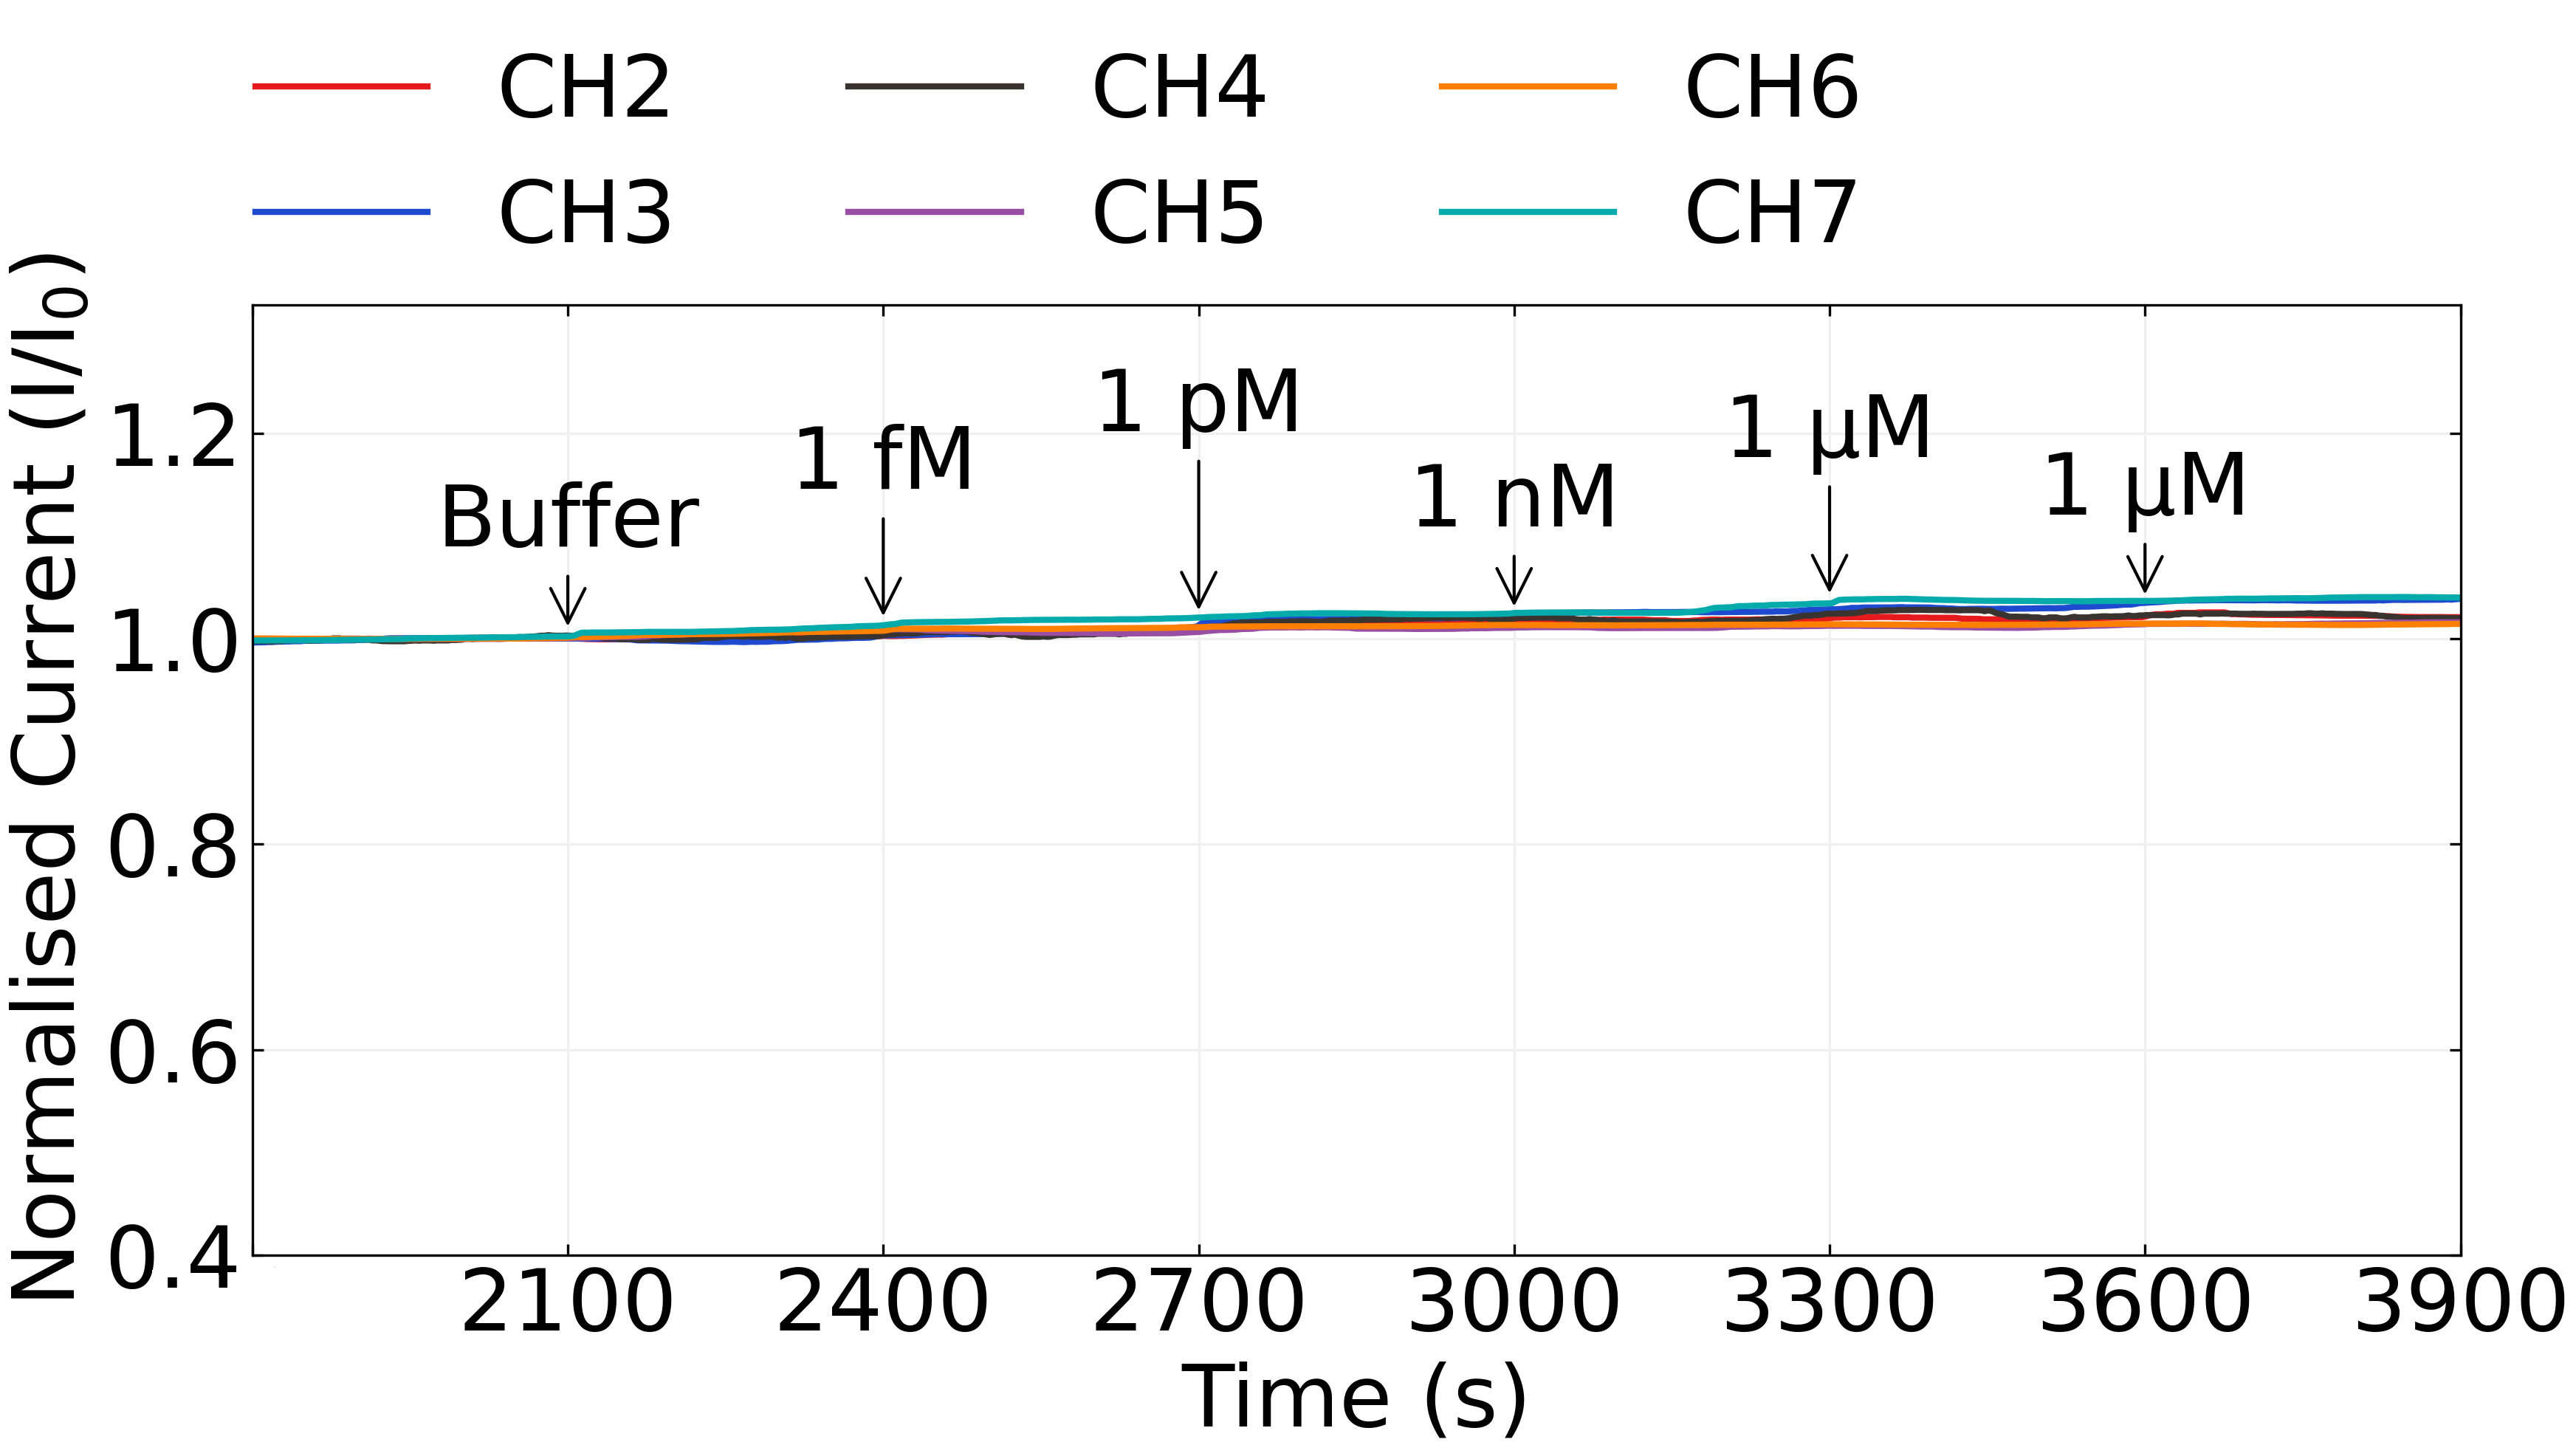
\includegraphics{figures/ch8/Q4C4_OR22a_Functionalised_2ndTimeSensingRun_48hrFridge_21_filtered_detrend_trunc_arrows_normalised.png}

}

}

\end{minipage}%
%
\begin{minipage}[t]{0.15\linewidth}

{\centering 

~

}

\end{minipage}%

\caption{\label{fig-OR22a-variability}The normalised sensing series of
another OR22a-functionalised device across six multiplexed channels,
where current data has been despiked and baseline drift removed. The
concentration of each 20 µL addition is indicated above the time of
addition. The same sensing series is shown in both (a) and (b), where a
moving median filter has been applied in (b).}

\end{figure}

Despite the successful detection of ethyl hexanoate by an OR22a
nanodisc-functionalised biosensor in
Section~\ref{sec-aqueous-sensing-EtHex}, it was found that this
behaviour was not readily reproducible. The results from the previous
section were not repeated when using the same procedure for fabrication
of devices alongside an identical functionalisation process with the
same batch of OR22a nanodiscs (ND-OR22a-SB018). The ethyl hexanoate
sensing sequence from six functionalised device channels is shown in
Figure~\ref{fig-OR22a-variability}. Figure~\ref{fig-OR22a-variability}
(a) has been left unfiltered to illustrate the variation in behaviour
between channels, while Figure~\ref{fig-OR22a-variability} (b) has been
prepared in the same manner as Figure~\ref{fig-OR22a-sensing-series}
(a). The current response to each analyte addition is similar to that
seen after the initial addition without ethyl hexanoate present. The
largest contributing factor to current change appears to be drift.
Unlike the clear decreases in current subsequent to ethyl hexanoate
additions seen in Figure~\ref{fig-OR22a-sensing-series} (a), no
decreases are seen in Figure~\ref{fig-OR22a-variability} (b) to any
ethyl hexanoate solution addition.

\begin{figure}

\begin{minipage}[t]{0.03\linewidth}

{\centering 

\raisebox{-\height}{


\includegraphics{figures/(a).png}

}

}

\end{minipage}%
%
\begin{minipage}[t]{0.01\linewidth}

{\centering 

~

}

\end{minipage}%
%
\begin{minipage}[t]{0.45\linewidth}

{\centering 

\raisebox{-\height}{

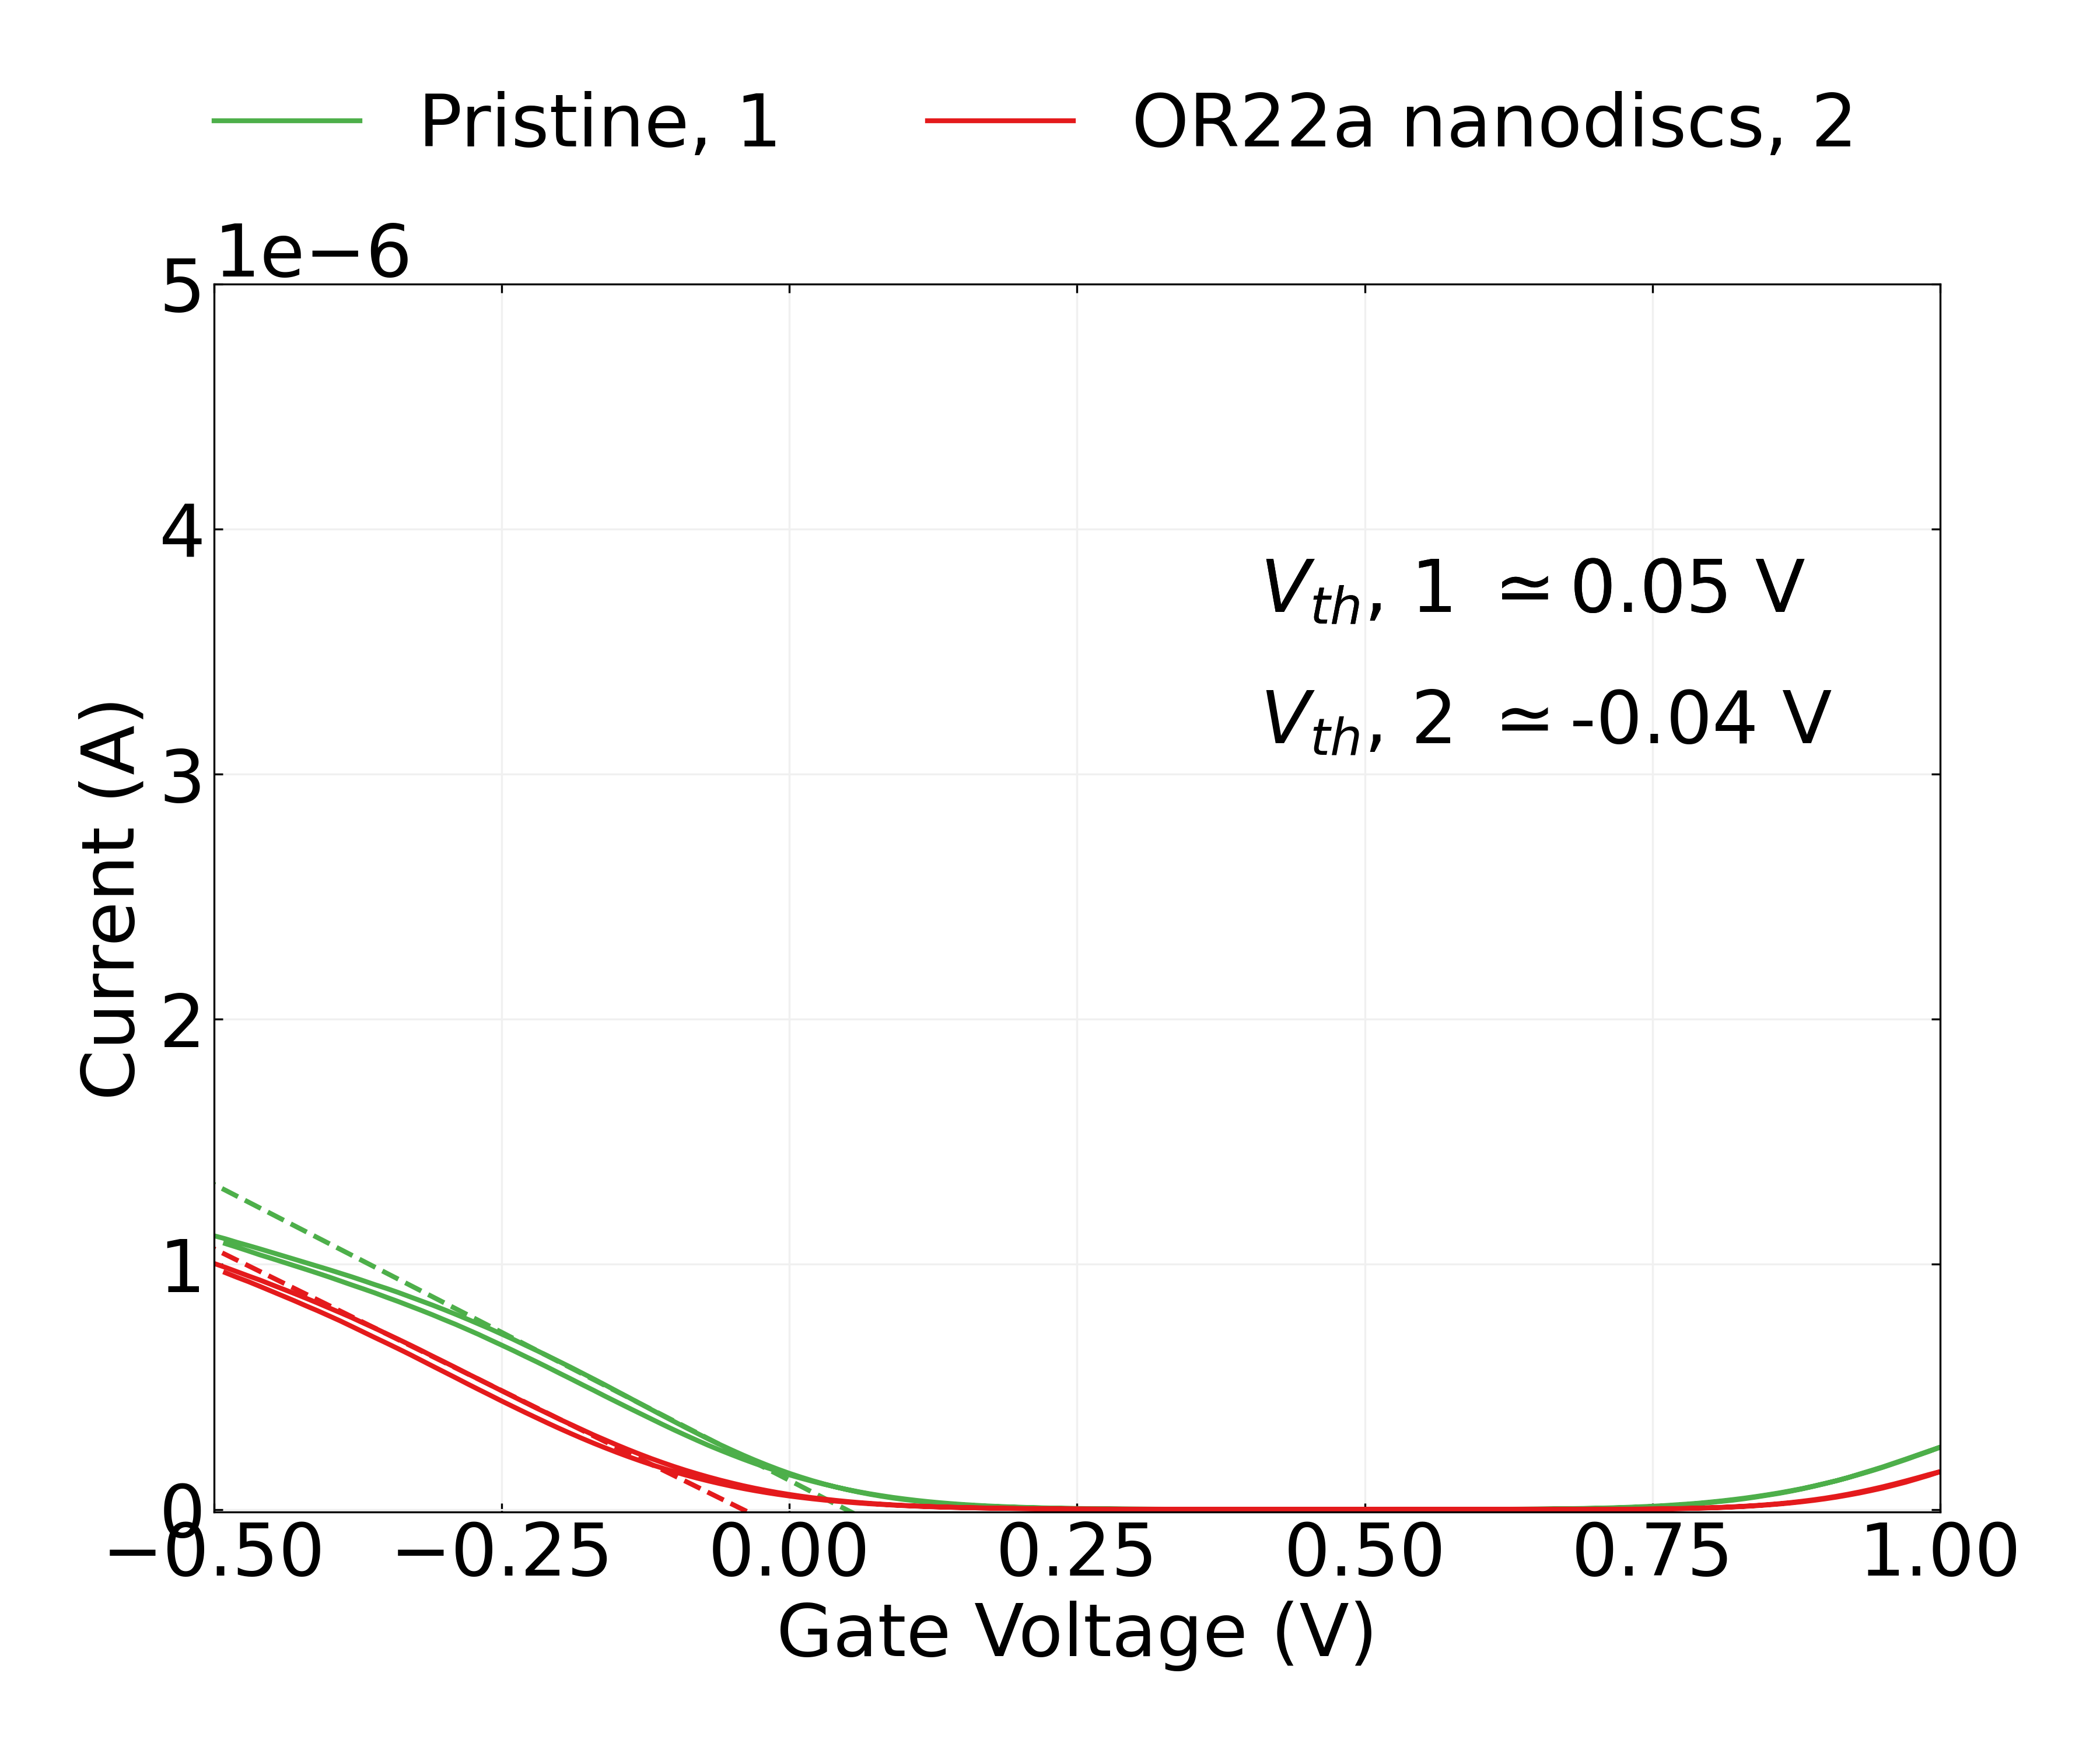
\includegraphics{figures/ch8/Q4C4_ch2.png}

}

}

\end{minipage}%
%
\begin{minipage}[t]{0.01\linewidth}

{\centering 

~

}

\end{minipage}%
%
\begin{minipage}[t]{0.03\linewidth}

{\centering 

\raisebox{-\height}{


\includegraphics{figures/(b).png}

}

}

\end{minipage}%
%
\begin{minipage}[t]{0.01\linewidth}

{\centering 

~

}

\end{minipage}%
%
\begin{minipage}[t]{0.45\linewidth}

{\centering 

\raisebox{-\height}{

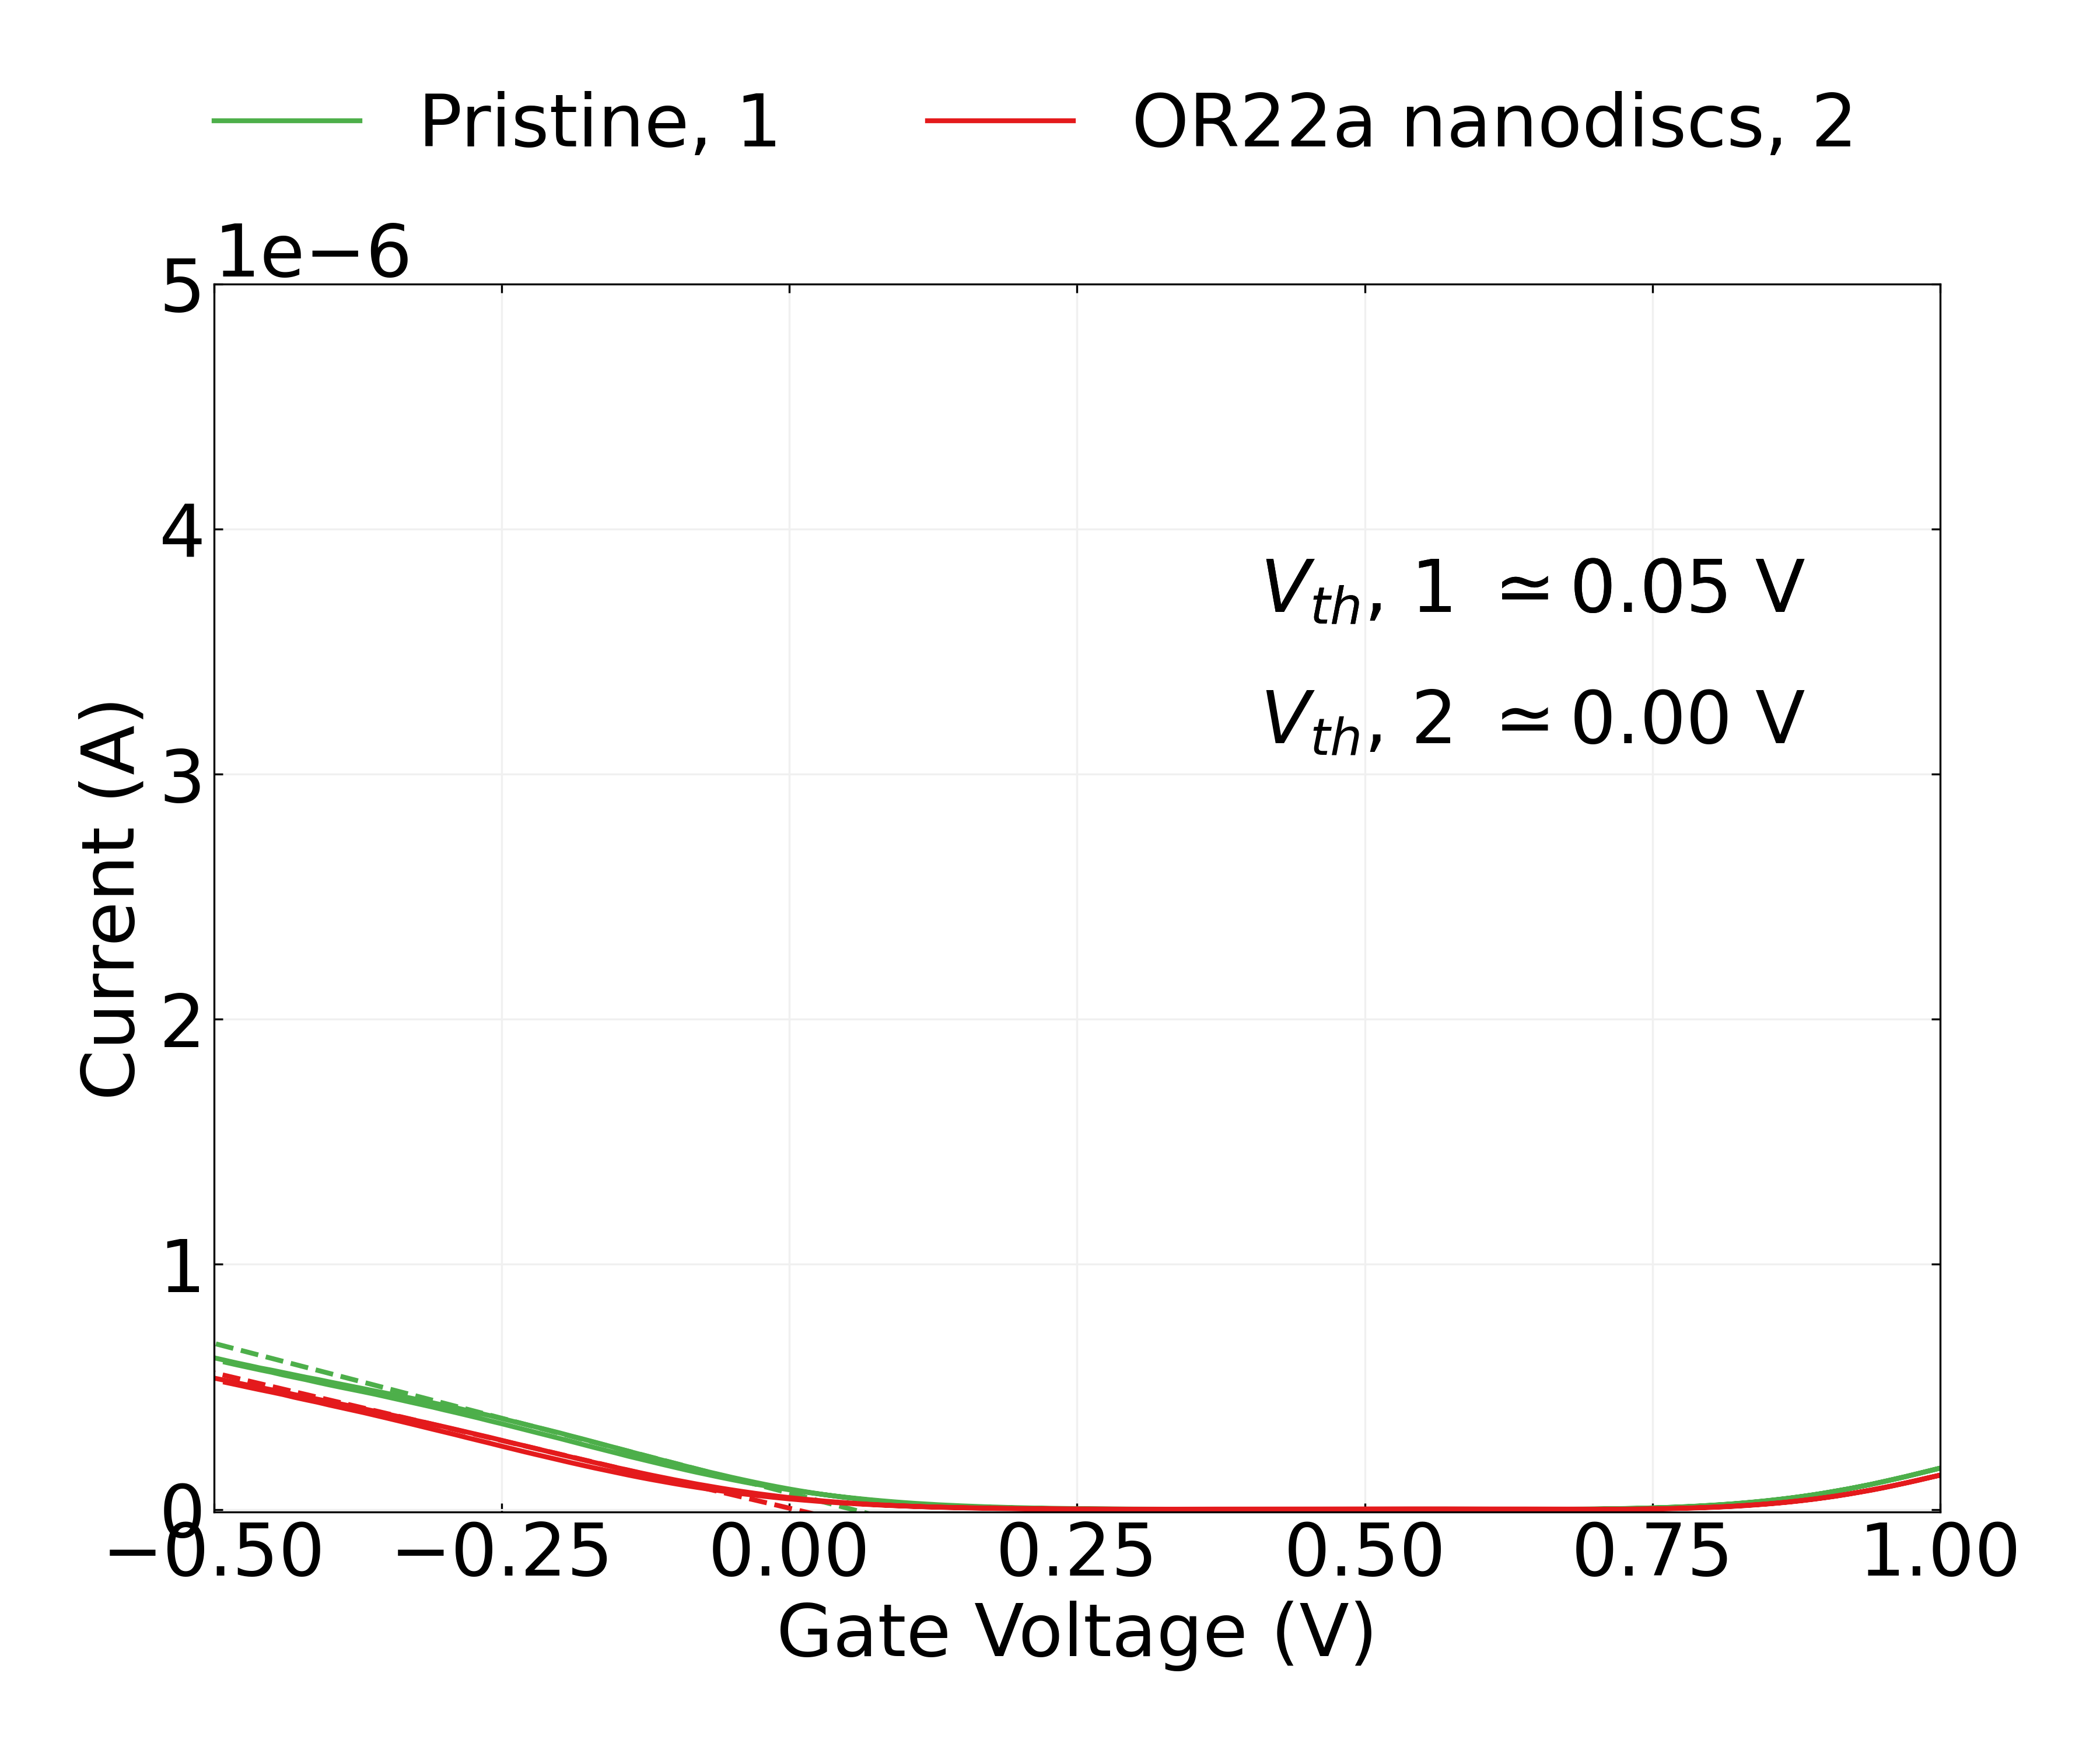
\includegraphics{figures/ch8/Q4C4_ch3.png}

}

}

\end{minipage}%
%
\begin{minipage}[t]{0.01\linewidth}

{\centering 

~

}

\end{minipage}%
\newline
\begin{minipage}[t]{0.03\linewidth}

{\centering 

\raisebox{-\height}{


\includegraphics{figures/(c).png}

}

}

\end{minipage}%
%
\begin{minipage}[t]{0.01\linewidth}

{\centering 

~

}

\end{minipage}%
%
\begin{minipage}[t]{0.45\linewidth}

{\centering 

\raisebox{-\height}{

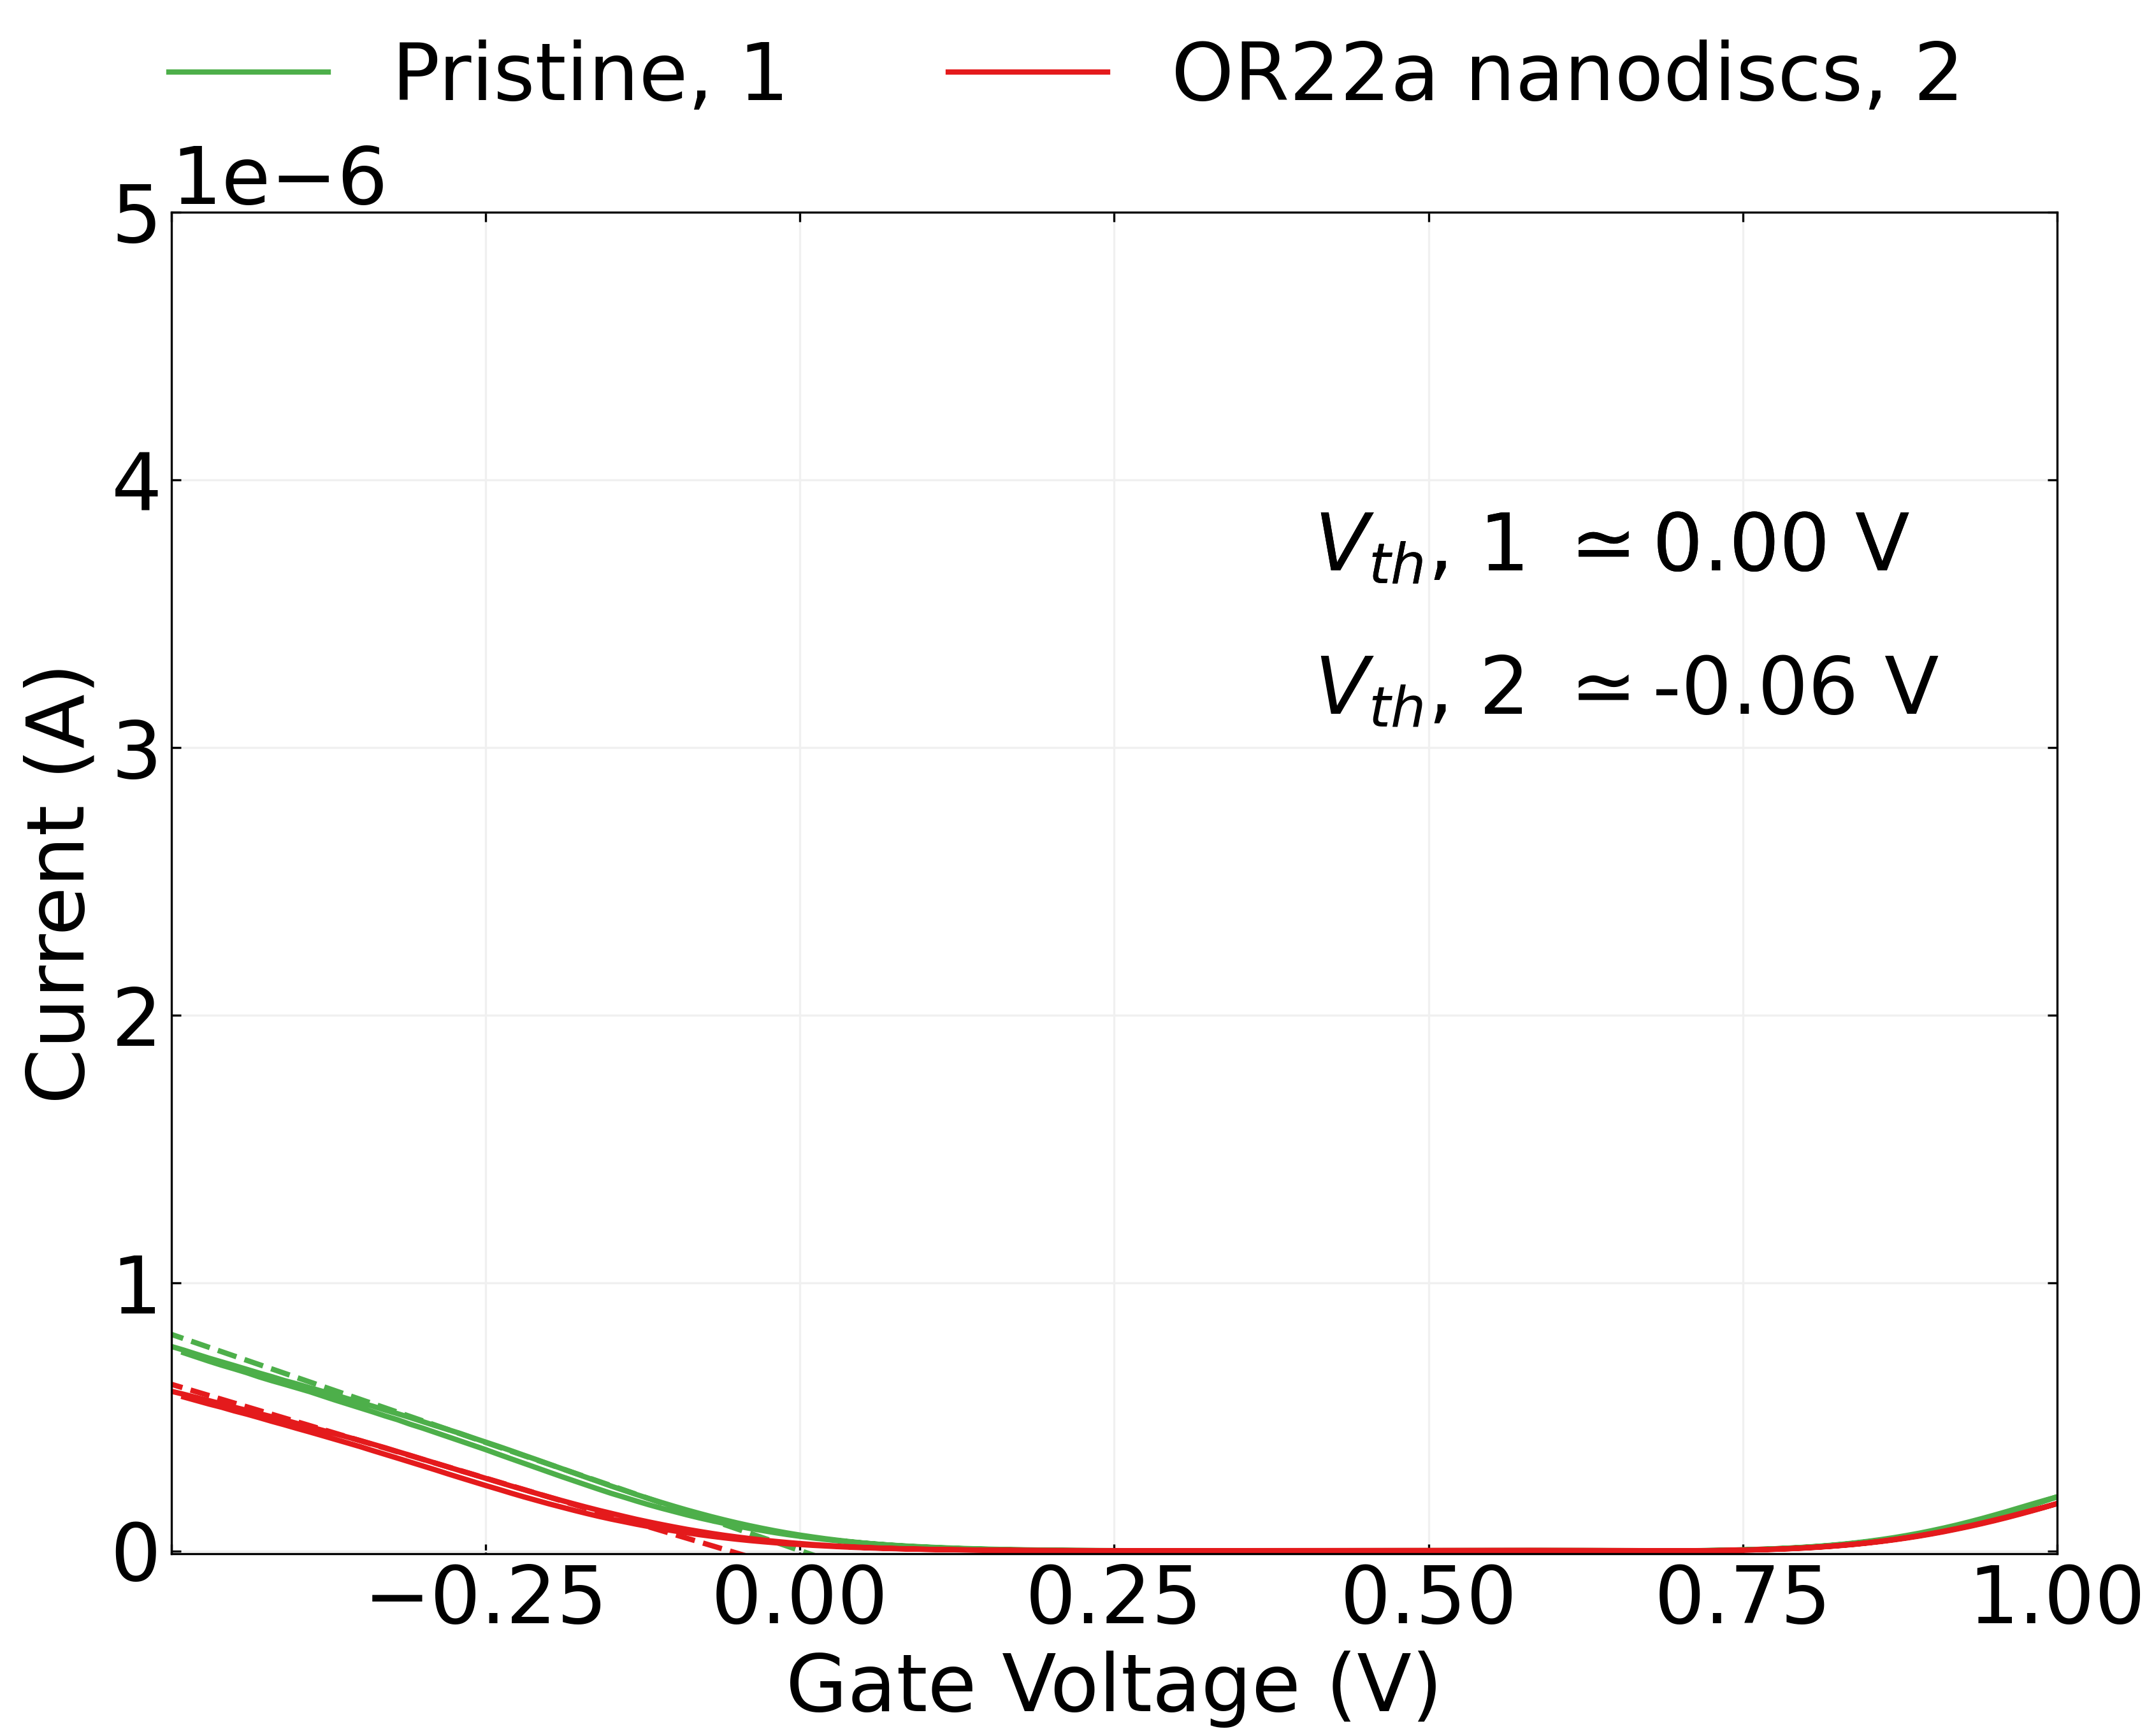
\includegraphics{figures/ch8/Q4C4_ch4.png}

}

}

\end{minipage}%
%
\begin{minipage}[t]{0.01\linewidth}

{\centering 

~

}

\end{minipage}%
%
\begin{minipage}[t]{0.03\linewidth}

{\centering 

\raisebox{-\height}{


\includegraphics{figures/(d).png}

}

}

\end{minipage}%
%
\begin{minipage}[t]{0.01\linewidth}

{\centering 

~

}

\end{minipage}%
%
\begin{minipage}[t]{0.45\linewidth}

{\centering 

\raisebox{-\height}{

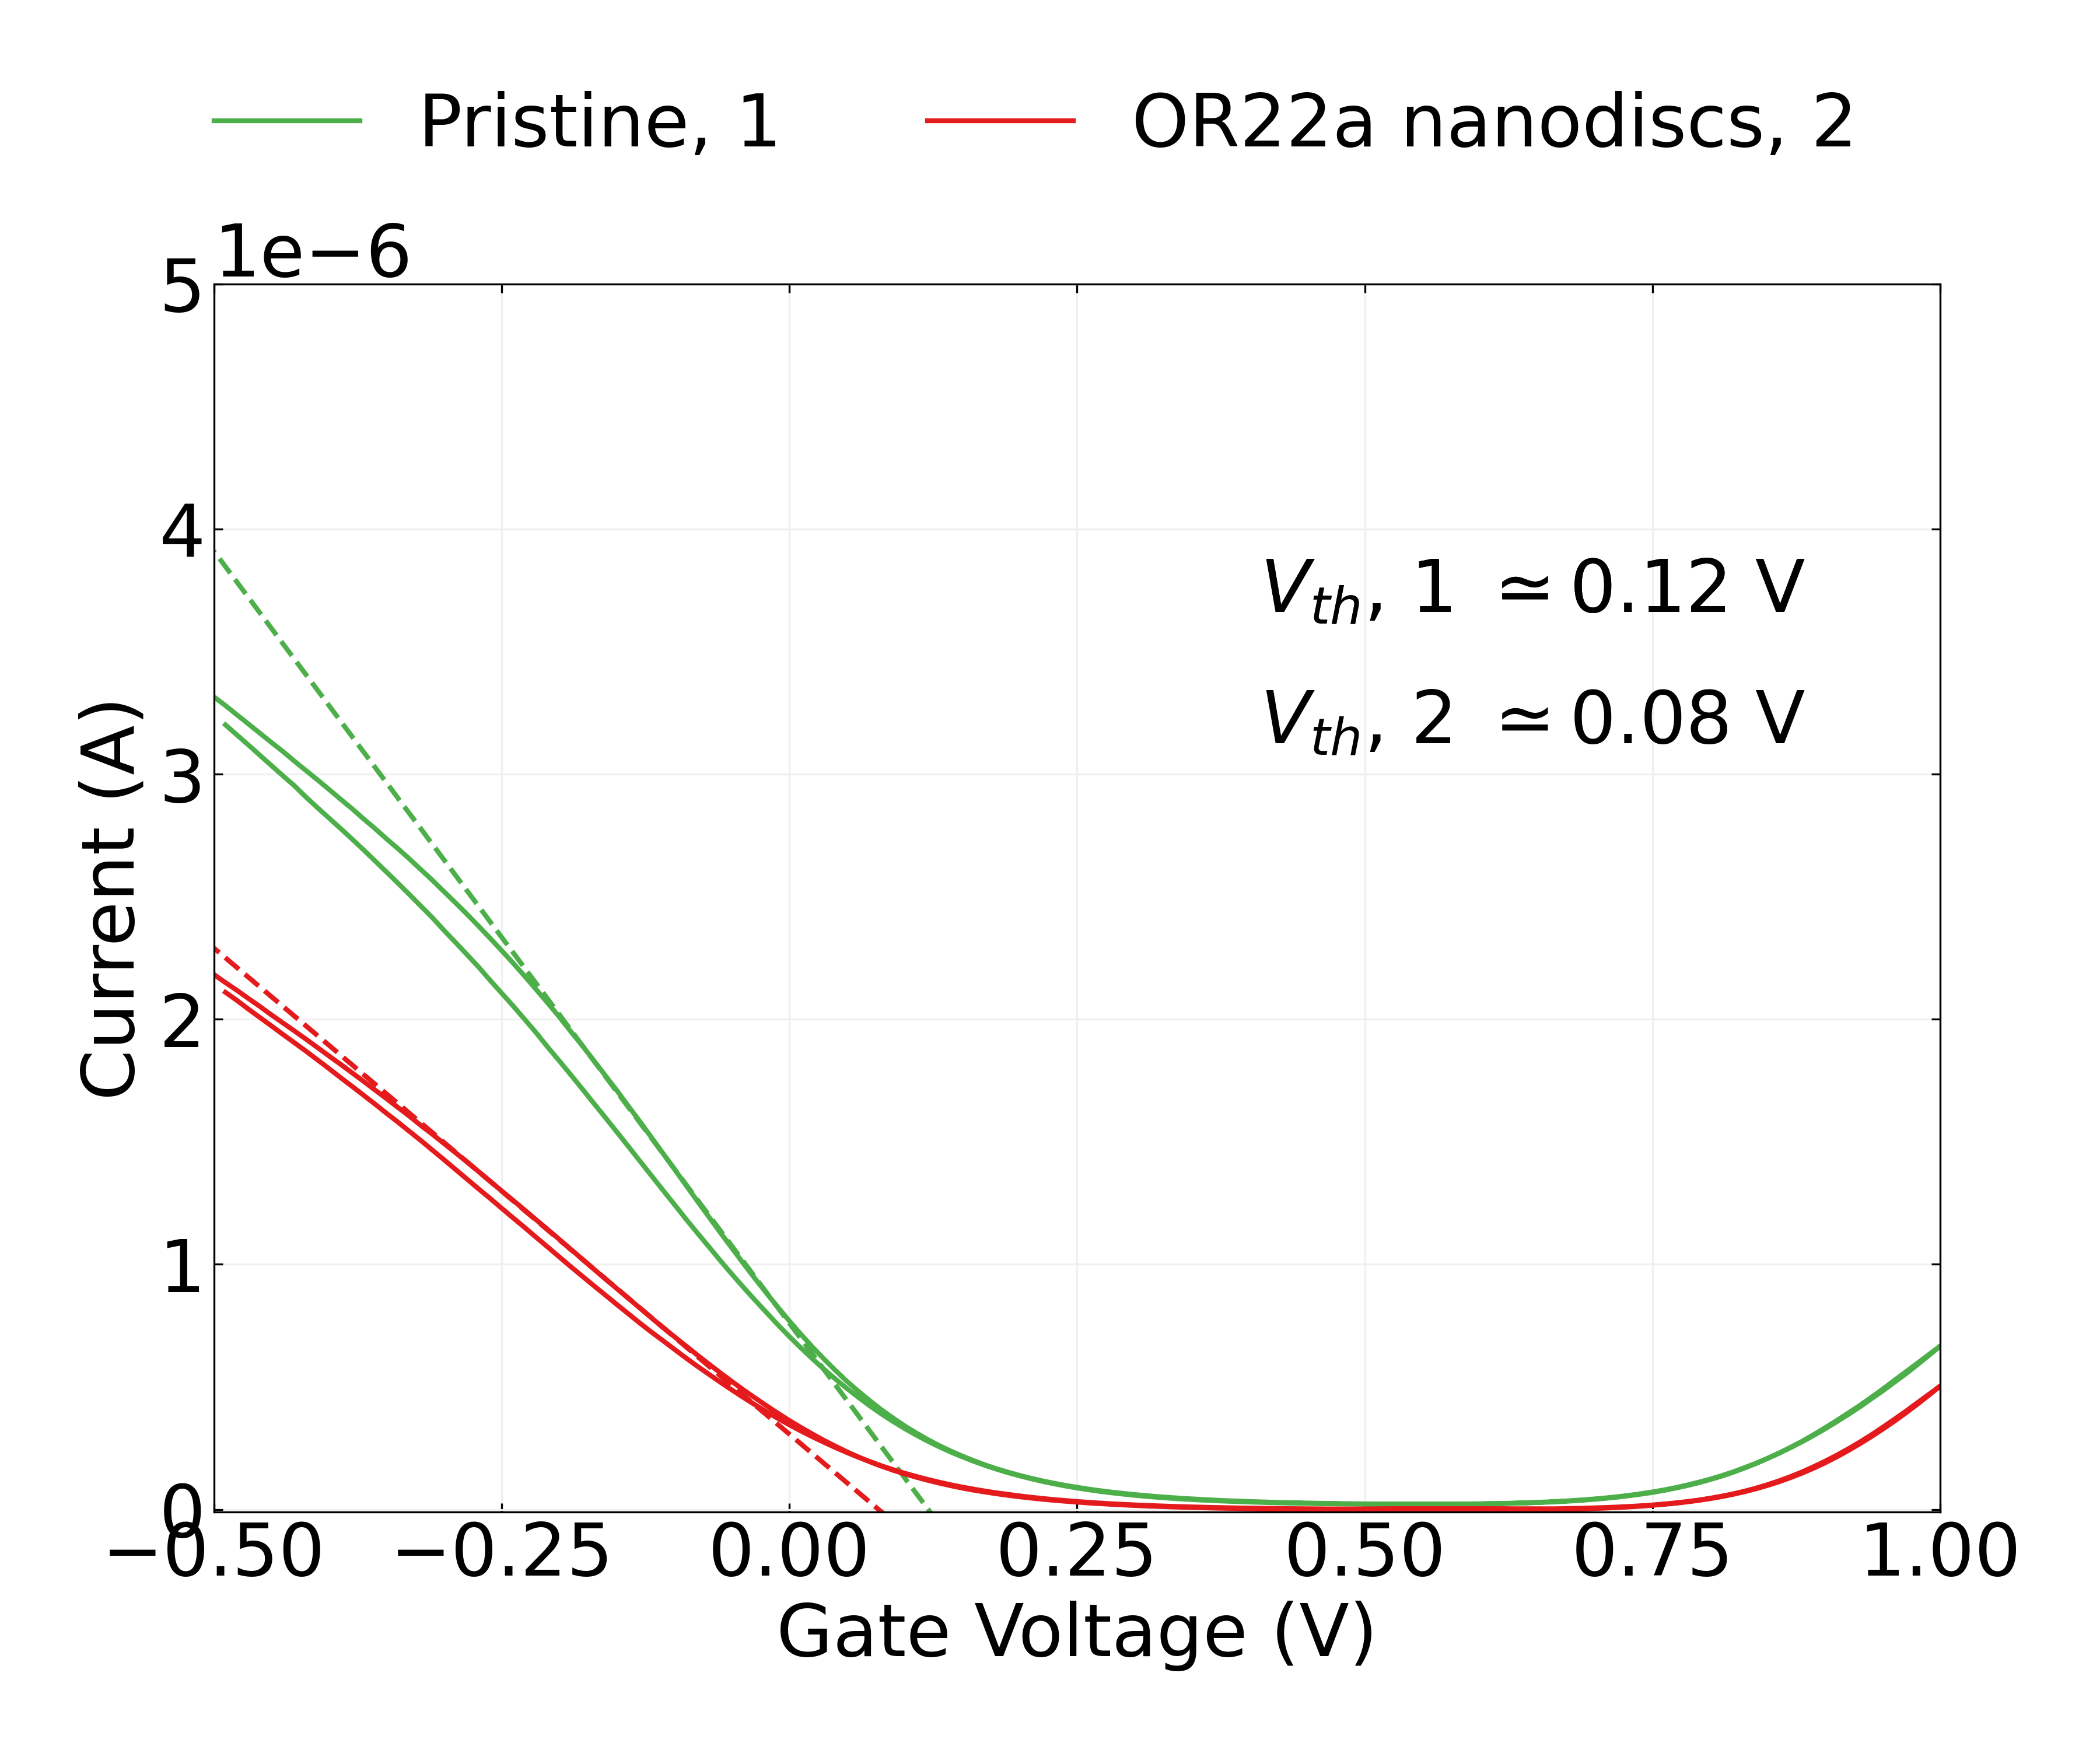
\includegraphics{figures/ch8/Q4C4_ch5.png}

}

}

\end{minipage}%
%
\begin{minipage}[t]{0.01\linewidth}

{\centering 

~

}

\end{minipage}%
\newline
\begin{minipage}[t]{0.03\linewidth}

{\centering 

\raisebox{-\height}{

\includegraphics{figures/(e).png}

}

}

\end{minipage}%
%
\begin{minipage}[t]{0.01\linewidth}

{\centering 

~

}

\end{minipage}%
%
\begin{minipage}[t]{0.45\linewidth}

{\centering 

\raisebox{-\height}{

\includegraphics{figures/ch8/Q4C4_ch6.png}

}

}

\end{minipage}%
%
\begin{minipage}[t]{0.01\linewidth}

{\centering 

~

}

\end{minipage}%
%
\begin{minipage}[t]{0.03\linewidth}

{\centering 

\raisebox{-\height}{

\includegraphics{figures/(f).png}

}

}

\end{minipage}%
%
\begin{minipage}[t]{0.01\linewidth}

{\centering 

~

}

\end{minipage}%
%
\begin{minipage}[t]{0.45\linewidth}

{\centering 

\raisebox{-\height}{

\includegraphics{figures/ch8/Q4C4_ch7.png}

}

}

\end{minipage}%
%
\begin{minipage}[t]{0.01\linewidth}

{\centering 

~

}

\end{minipage}%

\caption{\label{fig-OR22a-variability-TX}Liquid-gated carbon nanotube
network device transfer characteristics before and after OR22a nanodisc
functionalisation. Source-drain current was \(V_{ds}\) = 100 mV for both
the forward and reverse sweep. Each subfigure (a)-(f) corresponds to a
different channel of the functionalised device; (a) corresponds to
channel 2, (b) corresponds to channel 3, (c) corresponds to channel 4,
(d) corresponds to channel 5, (e) corresponds to channel 6 and (f)
corresponds to channel 7. The dashed line shown is tangent to the
subthreshold slope of the characteristic curve. The threshold voltage
corresponding to the intercept of this slope with the x-axis is shown
for each transfer characteristic curve.}

\end{figure}

\begin{figure}

{\centering \includegraphics[width=0.5\textwidth,height=\textheight]{figures/ch8/Q4C4_CH6_PostSensing_OR22a_Func_AFM100670_00693.png}

}

\caption{\label{fig-OR22a-variability-AFM}An atomic force microscope
image of channel 6 from the OR22a nanodisc functionalised device which
showed no response to ethyl hexanoate.}

\end{figure}

\begin{figure}

\begin{minipage}[t]{0.03\linewidth}

{\centering 

\raisebox{-\height}{

\includegraphics{figures/(a).png}

}

}

\end{minipage}%
%
\begin{minipage}[t]{0.01\linewidth}

{\centering 

~

}

\end{minipage}%
%
\begin{minipage}[t]{0.45\linewidth}

{\centering 

\raisebox{-\height}{

\includegraphics{figures/ch8/Q4C4_CH6_PostSensing_OR22a_Func_AFM100670_00693_mask.png}

}

}

\end{minipage}%
%
\begin{minipage}[t]{0.01\linewidth}

{\centering 

~

}

\end{minipage}%
%
\begin{minipage}[t]{0.03\linewidth}

{\centering 

\raisebox{-\height}{

\includegraphics{figures/(b).png}

}

}

\end{minipage}%
%
\begin{minipage}[t]{0.01\linewidth}

{\centering 

~

}

\end{minipage}%
%
\begin{minipage}[t]{0.45\linewidth}

{\centering 

\raisebox{-\height}{

\includegraphics{figures/ch8/Q4C4_CH6_PostSensing_OR22a_Func_AFM100670_00693_12.5nm_crosssection.png}

}

}

\end{minipage}%
%
\begin{minipage}[t]{0.01\linewidth}

{\centering 

~

}

\end{minipage}%

\caption{\label{fig-OR22a-variability-AFM-comparison}The mask used to
find the average substrate height of the functionalised channel 6 is
shown in (a), with the substrate highlighted green. The bounds of the
colour map have been lowered in (a), as colour mapping over the full
height range makes it difficult to clearly distinguish between sub-20 nm
features and the substrate. A binary representation of the atomic force
microscope image with a threshold height of 12.5 nm is shown in (b).}

\end{figure}

Liquid-gated electrical characteristics were taken of each sensing
channel from this device before and after functionalisation with OR22a
nanodiscs, in the same manner as
Section~\ref{sec-aqueous-sensing-EtHex}. These characteristics are shown
in Figure~\ref{fig-OR22a-variability-TX}. The average threshold shift
was \(-0.06\pm0.02\), the same as that of a device functionalised with
PBASE in methanol without subsequent functionalisation with OR22a
nanodiscs. To test whether protein was present on the channel, an atomic
force microscope image was taken of channel 6, as shown in
Figure~\ref{fig-OR22a-variability-AFM}. The same image analysis as in
Section~\ref{sec-aqueous-sensing-EtHex} was performed, with the
substrate mask shown in
Figure~\ref{fig-OR22a-variability-AFM-comparison} (a) giving an average
substrate height of \(3.8\pm0.4\). A binary representation of the image
with a 12.5 nm threshold, 8.7 nm above the average substrate height, is
shown in Figure~\ref{fig-OR22a-variability-AFM-comparison} (b). As with
the functionalised device in Figure~\ref{fig-crosssection} (b),
Figure~\ref{fig-OR22a-variability-AFM-comparison} (b) shows clustering
of features, many of which are larger than 50 nm across. It seems,
therefore, that nanodisc aggregates up to 27.5 nm high are present on
channel 6, despite the lack of a significant threshold shift as a result
of functionalisation.

\begin{figure}

{\centering \includegraphics[width=0.5\textwidth,height=\textheight]{figures/ch8/00161_noPBASE.png}

}

\caption{\label{fig-OR22a-noPBASE-AFM}An atomic force microscope image
of a carbon nanotube film submerged in OR22a nanodiscs for 1 hour
without prior exposure to PBASE or methanol.}

\end{figure}

\begin{figure}

\begin{minipage}[t]{0.03\linewidth}

{\centering 

\raisebox{-\height}{

\includegraphics{figures/(a).png}

}

}

\end{minipage}%
%
\begin{minipage}[t]{0.01\linewidth}

{\centering 

~

}

\end{minipage}%
%
\begin{minipage}[t]{0.45\linewidth}

{\centering 

\raisebox{-\height}{

\includegraphics{figures/ch8/Ned_Q16D2_W4_OR22a1_noPBASE_sensing_2.5micron_256px_00462_20210921_mask.png}

}

}

\end{minipage}%
%
\begin{minipage}[t]{0.01\linewidth}

{\centering 

~

}

\end{minipage}%
%
\begin{minipage}[t]{0.03\linewidth}

{\centering 

\raisebox{-\height}{

\includegraphics{figures/(b).png}

}

}

\end{minipage}%
%
\begin{minipage}[t]{0.01\linewidth}

{\centering 

~

}

\end{minipage}%
%
\begin{minipage}[t]{0.45\linewidth}

{\centering 

\raisebox{-\height}{

\includegraphics{figures/ch8/Ned_Q16D2_W4_OR22a1_noPBASE_sensing_2.5micron_256px_00462_20210921_crosssection.png}

}

}

\end{minipage}%
%
\begin{minipage}[t]{0.01\linewidth}

{\centering 

~

}

\end{minipage}%

\caption{\label{fig-OR22a-noPBASE-AFM-comparison}The binary
representation of the network, with a height threshold of 12.8 nm
(average substrate height = 4.1 nm), is shown in (b).}

\end{figure}

\begin{figure}

\begin{minipage}[t]{0.03\linewidth}

{\centering 

\raisebox{-\height}{

\includegraphics{figures/(a).png}

}

}

\end{minipage}%
%
\begin{minipage}[t]{0.01\linewidth}

{\centering 

~

}

\end{minipage}%
%
\begin{minipage}[t]{0.45\linewidth}

{\centering 

\raisebox{-\height}{

\includegraphics{figures/ch8/Q4C8_ch4_without_gate_current.png}

}

}

\end{minipage}%
%
\begin{minipage}[t]{0.03\linewidth}

{\centering 

~

}

\end{minipage}%
%
\begin{minipage}[t]{0.03\linewidth}

{\centering 

\raisebox{-\height}{

\includegraphics{figures/(b).png}

}

}

\end{minipage}%
%
\begin{minipage}[t]{0.45\linewidth}

{\centering 

\raisebox{-\height}{

\includegraphics{figures/ch8/Q4C8_filtered_detrend_trunc_arrows_normalised.png}

}

}

\end{minipage}%

\caption{\label{fig-OR22a-variability-TX-comparison}The device
characteristics in (a) are from channel 4 of the device placed in OR22a
nanodisc solution for 1 hour without prior exposure to PBASE or methanol
before and after functionalisation. Real-time sampling using this
channel is shown in (b). A 20 µL addition of 1\% v/v DMSO 1XPBS was made
at 200 s. Subsequently, 20 µL additions of ethyl hexanoate diluted in
1\% v/v DMSO 1XPBS were made at 400 s, 600 s, 800 s and 1000 s and 1200
s, with the concentration of each addition indicated above the time of
addition.}

\end{figure}

Both OR nanodisc and empty nanodisc attachment via PBASE have been shown
to cause significant gating of the network
(Section~\ref{sec-aqueous-sensing-EtHex}). Therefore, it might be
reasoned that the lack of a gating effect, but with nanodiscs present,
results from a direct attachment mechanism circumventing the PBASE
linker. The amine group on proteins can be attached directly onto carbon
nanotubes by adsorption, although this attachment is relatively weak
\autocite{Bradley2004}. Figure~\ref{fig-OR22a-noPBASE-AFM} shows an AFM
image of a carbon nanotube network film after submersion in a 10 µL/mL
OR22a nanodisc in PBS solution for 1 hour (batch NDOR22a-0016-1),
without prior exposure to PBASE in methanol.
Figure~\ref{fig-OR22a-noPBASE-AFM-comparison} shows the substrate mask
in (a) and a binary representation of this AFM with nanodisc aggregates
clearly visible in (b). In
Figure~\ref{fig-OR22a-variability-TX-comparison} (a), the negative
threshold shift of a channel modified in this way was -0.27 V, similar
in size to the shift due to functionalisation seen for the working
biosensor.

The attachment of nanodiscs in 1XPBS may seem surprising, given that the
fluorescence microscopy work in
Section~\ref{sec-working-PBASE-functionalisation} indicates no GFP-OR
present after functionalisation without PBASE. However, this device
channel did not work as a sensor when tested with ethyl hexanoate.
Figure~\ref{fig-OR22a-variability-TX-comparison} (b) shows a small,
positive current response to additions of ethyl hexanoate diluted in 1\%
v/v DMSO 1XPBS, which may result from the weakly attached OR22a
nanodiscs being mechanically removed by the pressure of each addition on
the device channels.

An explanation is required for the seemingly contradictory situation
where nanodiscs can be present on a device channel without significant
gating effects. The most straightforward explanation is that no reliable
correlation exist between the two phenomena. Given the consistent
threshold shift results for various linker functionalisations seen in
\textbf{?@sec-noncovalent-functionalisation}, this scenario implies a
significant variation in protein structure and charge behaviour within a
single nanodisc batch, which seems unlikely. Another possibility is that
some type of surface coating is causing nanodiscs to not attach to
either PBASE or the carbon nanotubes. This surface coating might be
attractive, attaching to both nanodiscs and carbon nanotubes, but
forming a barrier layer between the two. Alternatively, this coating
might be repulsive, causing nanodiscs to attach weakly to the substrate
around the carbon nanotubes. Variations in the degree to which a network
is coated may then explain why the same functionalisation method might
work for one device but not another. The following section investigates
ways of eliminating possible sources of surface coating for more
reliable functionalisation results.

\hypertarget{sec-contamination}{%
\subsection{Potential Sources of Variability}\label{sec-contamination}}

Throughout the course of this thesis, multiple potential candidates for
the unwanted surface coating discussed in the previous section have been
identified. These include the surfactant used in carbon nanotube
deposition (\textbf{?@sec-pristine-morphology},
\textbf{?@sec-pristine-electrical-characterisation}), the solvent used
in functionalisation (\textbf{?@sec-PBASE-electrical-characterisation}),
residual photoresist (\textbf{?@sec-photoresist-contamination}), and the
hydrophobic layer which naturally forms on graphene and carbon nanotubes
in air (\textbf{?@sec-hydrophobicity}). Another possibility is that
PBASE itself is acting as a surface coating, which could result from
multilayer coverage restricting access by the odorant receptors to
directly attached PBASE (\textbf{?@sec-PBASE-attachment}).
Alternatively, PBASE may have hydrolysed into PBA prior to attachment,
forming an inert surface layer upon \(\pi\)-stacking around the carbon
nanotubes. However, no threshold shift directly attributable to PBA
attachment should occur (\textbf{?@sec-PBA-characterisation}), and this
is not what was observed when characterising the non-working device in
Section~\ref{sec-variability-biosensor}. To understand which of these
candidates is responsible for the significant variability in biosensor
functionality, the sensing procedure was performed with slight
variations on the biosensor fabrication and functionalisation
procedures. In each test, an individual element of one of these
procedures was altered to prevent the introduction of a specific surface
coating. The biosensor was then characterised and tested to see if it
would respond to its target odorant.

\hypertarget{spurious-responses}{%
\subsubsection*{Spurious Responses}\label{spurious-responses}}
\addcontentsline{toc}{subsubsection}{Spurious Responses}

Before testing to see if a surface coating was responsible for the lack
of response seen to ethyl hexanoate by the device in
Section~\ref{sec-variability-biosensor}, it was important to investigate
the possibility the signals seen in
Section~\ref{sec-EtHex-aqueous-sensing} were false positives. The highly
sensitive device channel could credibly respond to three different rapid
environmental changes occurring with each addition: the mechanical
action of the addition, a difference between the 0.5\% v/v DMSO in 1XPBS
containing the analyte and the 0.5\% v/v DMSO in 1XPBS already in the
well, or a direct response to analyte. It is important to eliminate the
first two possibilities to be certain that the device is responding to
analyte. The control series as it stands demonstrates responses cannot
be explained by mechanical action. All analyte solutions are prepared
simultaneously using the same 1XPBS, taking care to avoid
cross-contamination, so responses are unlikely to result from a
difference between the 1XPBS in the analyte solution and the 1XPBS in
the well. It then must be verified whether a functionalised device
channel will respond to a change in DMSO concentration, which is the
result of the DMSO concentration in an analyte addition being different
to the concentration in the PDMS well.

\begin{figure}

{\centering \includegraphics[width=0.7\textwidth,height=\textheight]{figures/ch8/NGW4_D7_OR22aliposome_sampling_220623_detrend_trunc_arrows_normalised.png}

}

\caption{\label{fig-DMSO-concentration}Response to changing the
concentration of DMSO in the PDMS well of a OR22a-functionalised sensor.
Source-drain current was set at \(V_{ds}\) = 100 mV while gate current
was set at \(V_g\) = 0 V. The well originally contained 100 µL of 1\%
v/v DMSO 1XPBS. 20 µL additions of DMSO in PBS were made at 3300 s and
3600 s.}

\end{figure}

Figure~\ref{fig-DMSO-concentration} shows that a increase in DMSO
concentration in the well from 1\% v/v to 2.5\% v/v leads to a steep
drop in current of 0.5\% \(-\) 1.5\% across two OR22a-functionalised
device channels. The gate current remained negligible across this time
period (\textless0.1\% of average drain current). Though the current
changes in Figure~\ref{fig-DMSO-concentration} share similarities with
other observed responses to analyte, they are significantly smaller than
the \textgreater2\% changes seen in
Section~\ref{sec-EtHex-aqueous-sensing}. Furthermore, precise
measurement of DMSO in analyte preparations means that a change in
proportion of DMSO in the well of this scale is unlikely. It therefore
seems improbable that a change in DMSO concentration is the primary
cause of these responses. However, the author recommends a slight
modification to the control series for a more robust experimental
baseline. For a device with 100 µL 0.5\% v/v DMSO 1XPBS in the well
after the first buffer addition at 100 s, a subsequent 20 µL addition of
1\% v/v DMSO 1XPBS at 200 s and 20 µL addition of 0\% v/v DMSO 1XPBS
addition at 300 s can be used to check for spurious responses due to
changing DMSO concentration, while ensuring the DMSO concentration in
the well is 0.5\% v/v after the control series.

\hypertarget{fabrication}{%
\subsubsection*{Fabrication}\label{fabrication}}
\addcontentsline{toc}{subsubsection}{Fabrication}

Two different approaches were trialled to eliminate possible surfactant
contamination, both of which drew heavily on previous methods used for
iOR biosensor fabrication \autocite{Murugathas2019b,Murugathas2020}.
Solvent-deposited carbon nanotube network and graphene devices were
fabricated as described in \textbf{?@sec-qw-processing}. The same
functionalisation process for each device was used as described in
Section~\ref{sec-working-PBASE-functionalisation} with OR22a nanodiscs.

\begin{figure}

\begin{minipage}[t]{0.11\linewidth}

{\centering 

~

}

\end{minipage}%
%
\begin{minipage}[t]{0.03\linewidth}

{\centering 

\raisebox{-\height}{

\includegraphics{figures/(a).png}

}

}

\end{minipage}%
%
\begin{minipage}[t]{0.01\linewidth}

{\centering 

~

}

\end{minipage}%
%
\begin{minipage}[t]{0.70\linewidth}

{\centering 

\raisebox{-\height}{

\includegraphics{figures/ch8/NTQ25C5_OR22a_sample_220126_detrend_trunc_arrows_normalised.png}

}

}

\end{minipage}%
%
\begin{minipage}[t]{0.15\linewidth}

{\centering 

~

}

\end{minipage}%
\newline
\begin{minipage}[t]{0.11\linewidth}

{\centering 

~

}

\end{minipage}%
%
\begin{minipage}[t]{0.03\linewidth}

{\centering 

\raisebox{-\height}{

\includegraphics{figures/(b).png}

}

}

\end{minipage}%
%
\begin{minipage}[t]{0.01\linewidth}

{\centering 

~

}

\end{minipage}%
%
\begin{minipage}[t]{0.70\linewidth}

{\centering 

\raisebox{-\height}{

\includegraphics{figures/ch8/NTQ25C5_OR22a_sample_220126_filtered_detrend_trunc_arrows_normalised.png}

}

}

\end{minipage}%
%
\begin{minipage}[t]{0.15\linewidth}

{\centering 

~

}

\end{minipage}%

\caption{\label{fig-solvent-deposited-sensing}The normalised sensing
series of the solvent-deposited, OR22a-functionalised device across six
multiplexed channels, where current data has been despiked and baseline
drift removed. Source-drain current was set at \(V_{ds}\) = 100 mV while
gate current was set at \(V_g\) = 0 V. The concentration of each 20 µL
addition is indicated above the time of addition. The same sensing
series is shown in both (a) and (b), where a moving median filter has
been applied in (b).}

\end{figure}

\begin{figure}

\begin{minipage}[t]{0.03\linewidth}

{\centering 

\raisebox{-\height}{

\includegraphics{figures/(a).png}

}

}

\end{minipage}%
%
\begin{minipage}[t]{0.01\linewidth}

{\centering 

~

}

\end{minipage}%
%
\begin{minipage}[t]{0.45\linewidth}

{\centering 

\raisebox{-\height}{

\includegraphics{figures/ch8/NTQ25C5_ch1.png}

}

}

\end{minipage}%
%
\begin{minipage}[t]{0.01\linewidth}

{\centering 

~

}

\end{minipage}%
%
\begin{minipage}[t]{0.03\linewidth}

{\centering 

\raisebox{-\height}{

\includegraphics{figures/(b).png}

}

}

\end{minipage}%
%
\begin{minipage}[t]{0.01\linewidth}

{\centering 

~

}

\end{minipage}%
%
\begin{minipage}[t]{0.45\linewidth}

{\centering 

\raisebox{-\height}{

\includegraphics{figures/ch8/NTQ25C5_ch2.png}

}

}

\end{minipage}%
%
\begin{minipage}[t]{0.01\linewidth}

{\centering 

~

}

\end{minipage}%
\newline
\begin{minipage}[t]{0.03\linewidth}

{\centering 

\raisebox{-\height}{

\includegraphics{figures/(c).png}

}

}

\end{minipage}%
%
\begin{minipage}[t]{0.01\linewidth}

{\centering 

~

}

\end{minipage}%
%
\begin{minipage}[t]{0.45\linewidth}

{\centering 

\raisebox{-\height}{

\includegraphics{figures/ch8/NTQ25C5_ch3.png}

}

}

\end{minipage}%
%
\begin{minipage}[t]{0.01\linewidth}

{\centering 

~

}

\end{minipage}%
%
\begin{minipage}[t]{0.03\linewidth}

{\centering 

\raisebox{-\height}{

\includegraphics{figures/(d).png}

}

}

\end{minipage}%
%
\begin{minipage}[t]{0.01\linewidth}

{\centering 

~

}

\end{minipage}%
%
\begin{minipage}[t]{0.45\linewidth}

{\centering 

\raisebox{-\height}{

\includegraphics{figures/ch8/NTQ25C5_ch4.png}

}

}

\end{minipage}%
%
\begin{minipage}[t]{0.01\linewidth}

{\centering 

~

}

\end{minipage}%
\newline
\begin{minipage}[t]{0.03\linewidth}

{\centering 

\raisebox{-\height}{

\includegraphics{figures/(e).png}

}

}

\end{minipage}%
%
\begin{minipage}[t]{0.01\linewidth}

{\centering 

~

}

\end{minipage}%
%
\begin{minipage}[t]{0.45\linewidth}

{\centering 

\raisebox{-\height}{

\includegraphics{figures/ch8/NTQ25C5_ch5.png}

}

}

\end{minipage}%
%
\begin{minipage}[t]{0.01\linewidth}

{\centering 

~

}

\end{minipage}%
%
\begin{minipage}[t]{0.03\linewidth}

{\centering 

\raisebox{-\height}{

\includegraphics{figures/(f).png}

}

}

\end{minipage}%
%
\begin{minipage}[t]{0.01\linewidth}

{\centering 

~

}

\end{minipage}%
%
\begin{minipage}[t]{0.45\linewidth}

{\centering 

\raisebox{-\height}{

\includegraphics{figures/ch8/NTQ25C5_ch6.png}

}

}

\end{minipage}%
%
\begin{minipage}[t]{0.01\linewidth}

{\centering 

~

}

\end{minipage}%

\caption{\label{fig-solvent-deposited-sensing-TX}Liquid-gated
solvent-deposited carbon nanotube device transfer characteristics before
and after OR22a nanodisc functionalisation. Source-drain current was
\(V_{ds}\) = 100 mV for both the forward and reverse sweep. (a)
corresponds to channel 2, (b) corresponds to channel 3, (c) corresponds
to channel 4, (d) corresponds to channel 5, (e) corresponds to channel 6
and (f) corresponds to channel 7. The dashed line shown is tangent to
the subthreshold slope of the characteristic curve. The threshold
voltage corresponding to the intercept of this slope with the x-axis is
shown for each transfer characteristic curve.}

\end{figure}

\begin{figure}

\begin{minipage}[t]{0.03\linewidth}

{\centering 

\raisebox{-\height}{

\includegraphics{figures/(a).png}

}

}

\end{minipage}%
%
\begin{minipage}[t]{0.01\linewidth}

{\centering 

~

}

\end{minipage}%
%
\begin{minipage}[t]{0.44\linewidth}

{\centering 

\raisebox{-\height}{

\includegraphics{figures/ch8/Ned_NTQ25C5_W4_20220126_00245_mask.png}

}

}

\end{minipage}%
%
\begin{minipage}[t]{0.01\linewidth}

{\centering 

~

}

\end{minipage}%
%
\begin{minipage}[t]{0.03\linewidth}

{\centering 

\raisebox{-\height}{

\includegraphics{figures/(b).png}

}

}

\end{minipage}%
%
\begin{minipage}[t]{0.01\linewidth}

{\centering 

~

}

\end{minipage}%
%
\begin{minipage}[t]{0.46\linewidth}

{\centering 

\raisebox{-\height}{

\includegraphics{figures/ch8/Ned_NTQ25C5_W4_20220126_00245_section.png}

}

}

\end{minipage}%
%
\begin{minipage}[t]{0.01\linewidth}

{\centering 

~

}

\end{minipage}%
\newline
\begin{minipage}[t]{0.03\linewidth}

{\centering 

\raisebox{-\height}{

\includegraphics{figures/(c).png}

}

}

\end{minipage}%
%
\begin{minipage}[t]{0.01\linewidth}

{\centering 

~

}

\end{minipage}%
%
\begin{minipage}[t]{0.45\linewidth}

{\centering 

\raisebox{-\height}{

\includegraphics{figures/ch8/Ned_NTQ13_D11_dep50min_OR22a_dep1hr_20210211_00089.png}

}

}

\end{minipage}%
%
\begin{minipage}[t]{0.01\linewidth}

{\centering 

~

}

\end{minipage}%
%
\begin{minipage}[t]{0.03\linewidth}

{\centering 

\raisebox{-\height}{

\includegraphics{figures/(d).png}

}

}

\end{minipage}%
%
\begin{minipage}[t]{0.01\linewidth}

{\centering 

~

}

\end{minipage}%
%
\begin{minipage}[t]{0.45\linewidth}

{\centering 

\raisebox{-\height}{

\includegraphics{figures/ch8/Ned_NTQ13_D11_dep50min_OR22a_dep1hr_20210211_00088.png}

}

}

\end{minipage}%
%
\begin{minipage}[t]{0.01\linewidth}

{\centering 

~

}

\end{minipage}%

\caption{\label{fig-solvent-deposited-AFM-comparison}An 2.5 µm
\(\times\) 2.5 µm atomic force microscope image of an OR22a nanodisc
functionalised solvent-deposited carbon nanotube film is shown in (a),
with the average substrate height highlighted green. A binary
representation of the atomic force microscope image with a threshold
height of 34.7 nm is shown in (b). 10 µm \(\times\) 10 µm and 50 µm
\(\times\) 50 µm atomic force microscope images of another film
functionalised in the same manner are shown in (c) and (d)
respectively.}

\end{figure}

The normalised sensing behaviour for the solvent-deposited carbon
nanotube device is shown in Figure~\ref{fig-solvent-deposited-sensing}.
The device shows a small current increase on four channels with the 10
fM ethyl hexanoate addition, and a small decrease on five channels with
the 100 fM EtHex addition. No current change exceeded 2\%, and as shown
in Figure~\ref{fig-solvent-deposited-sensing} (b), the current changes
appear negligible on the scale of the changes seen in
Section~\ref{sec-EtHex-aqueous-sensing}. The average threshold shift
from functionalisation was \(-0.02\pm0.01\) V, which indicates
attachment of PBASE but not nanodiscs. As the device was made using the
pre-2023 encapsulation mask, an AFM was taken of a separate film
modified in the same manner, shown in
Figure~\ref{fig-solvent-deposited-AFM-comparison} (a). The average
substrate height was \(11.3\pm0.9\) nm. A binary representation of the
image taken at the minimum height no spindle-like bundles were visible,
46.1 nm, is shown in Figure~\ref{fig-solvent-deposited-AFM-comparison}
(b). Attached nanodisc aggregations are clearly visible, and appear
closer in nature to those observed for an OR35a-functionalised film
\autocite{Murugathas2020} than previously seen in this work.
Figure~\ref{fig-solvent-deposited-AFM-comparison} (c) and (d) show that
over a larger scale these aggregations can be at least 330 nm tall,
forming large clusters which may indicate mutual interaction during
deposition.

\begin{figure}

\begin{minipage}[t]{0.03\linewidth}

{\centering 

\raisebox{-\height}{

\includegraphics{figures/(a).png}

}

}

\end{minipage}%
%
\begin{minipage}[t]{0.01\linewidth}

{\centering 

~

}

\end{minipage}%
%
\begin{minipage}[t]{0.45\linewidth}

{\centering 

\raisebox{-\height}{

\includegraphics{figures/ch8/Q3C3_ch6_PBASE_OR22a.png}

}

}

\end{minipage}%
%
\begin{minipage}[t]{0.01\linewidth}

{\centering 

~

}

\end{minipage}%
%
\begin{minipage}[t]{0.03\linewidth}

{\centering 

\raisebox{-\height}{

\includegraphics{figures/(b).png}

}

}

\end{minipage}%
%
\begin{minipage}[t]{0.01\linewidth}

{\centering 

~

}

\end{minipage}%
%
\begin{minipage}[t]{0.45\linewidth}

{\centering 

\raisebox{-\height}{

\includegraphics{figures/ch8/Q3C9_ch4_noPBASE_OR22a.png}

}

}

\end{minipage}%
%
\begin{minipage}[t]{0.01\linewidth}

{\centering 

~

}

\end{minipage}%

\caption{\label{fig-graphene-sensing-TX}Liquid-gated graphene device
transfer characteristics before and after OR22a nanodisc
functionalisation. Source-drain current was \(V_{ds}\) = 100 mV for both
the forward and reverse sweep. (a) corresponds to a device
functionalised, where (a) was functionalised using the standard method
while (b) was functionalised without submerging the device in PBASE and
methanol. The shift in Dirac point resulting from functionalisation is
also shown for each device.}

\end{figure}

\begin{figure}

\begin{minipage}[t]{0.03\linewidth}

{\centering 

\raisebox{-\height}{

\includegraphics{figures/(a).png}

}

}

\end{minipage}%
%
\begin{minipage}[t]{0.01\linewidth}

{\centering 

~

}

\end{minipage}%
%
\begin{minipage}[t]{0.46\linewidth}

{\centering 

\raisebox{-\height}{

\includegraphics{figures/ch8/Ned_NG007_w3_pristine_00087_20210428.png}

}

}

\end{minipage}%
%
\begin{minipage}[t]{0.03\linewidth}

{\centering 

\raisebox{-\height}{

\includegraphics{figures/(b).png}

}

}

\end{minipage}%
%
\begin{minipage}[t]{0.01\linewidth}

{\centering 

~

}

\end{minipage}%
%
\begin{minipage}[t]{0.46\linewidth}

{\centering 

\raisebox{-\height}{

\includegraphics{figures/ch8/Ned_NGW3D4_OR22a_w1_00243_20210802.png}

}

}

\end{minipage}%
%
\begin{minipage}[t]{0.01\linewidth}

{\centering 

~

}

\end{minipage}%

\caption{\label{fig-graphene-AFM-comparison}2.5 µm \(\times\) 2.5 µm
atomic force microscope images of (a) a monolayer graphene film on
SiO\(_2\) and (b) a graphene film after OR22a nanodisc
functionalisation.}

\end{figure}

The electrical characteristics of a graphene device channel before and
after functionalisation with OR22a nanodiscs in the manner outlined
previously are shown in Figure~\ref{fig-graphene-sensing-TX} (a),
showing an order of magnitude decrease in on-current and a negatively
shifted Dirac point with functionalisation, as seen previously for
working OR22a nanodisc GFET biosensors \autocite{Murugathas2020}.
Figure~\ref{fig-graphene-sensing-TX} (b) shows when the process is
repeated on another device without initial exposure to PBASE and
methanol, a larger negative shift in the Dirac point is observed. It
appears the initial functionalisation with PBASE and methanol decreases
the charge transferred to the graphene when the nanodiscs are
introduced; the difference between these two surface modifications is
analogous to that seen for the carbon nanotube devices in
Section~\ref{sec-variability-biosensor}. A pristine graphene surface and
a OR22a-functionalised graphene surface are shown in
Figure~\ref{fig-graphene-AFM-comparison} (a) and (b) respectively.
Graphene folds of up to 7.3 nm in height are visible on the right hand
side of Figure~\ref{fig-graphene-AFM-comparison} (a). When
functionalised with OR22a nanodiscs, the surface is densely coated with
nanodisc aggregates up to \(\sim\) 250 nm across and \(\sim\) 30 nm
tall. These nanodiscs are a similar height and size to those observed by
Murugathas \emph{et al.} \autocite{Murugathas2020}.

\begin{figure}

{\centering \includegraphics[width=0.7\textwidth,height=\textheight]{figures/ch8/Q3C3_filtered_trunc_arrows_normalised.png}

}

\caption{\label{fig-graphene-sensing}A normalised ethyl hexanoate
sensing series taken with a OR22a-functionalised graphene device.
Source-drain current was set at \(V_{ds}\) = 100 mV while gate current
was set at \(V_g\) = 0 V. The concentration of each 20 µL addition is
indicated above the time of addition, with additions made at 500 s, 1000
s, 1500 s, 2000 s and 2500 s.}

\end{figure}

Both the transfer characteristics and atomic force microscope image
indicates widespread attachment of nanodiscs. However, the normalised
current data from a OR22a nanodisc graphene field-effect transistor in
Figure~\ref{fig-graphene-sensing} shows current changes of \textless1\%
in response to ethyl hexanoate additions. This contrasts with the OR22a
nanodisc-functionalised graphene device behaviour observed by Murugathas
\emph{et al.}, where target analyte additions with concentration above
10 fM consistently caused current changes of above 2\%
\autocite{Murugathas2020}. Again, there appears to be an unresolved
functionalisation issue that is not clearly captured either by the
atomic force microscope images or the transfer characteristics before
and after functionalisation of the graphene devices.

It appears that avoiding the use of surfactant on the transducer element
is not sufficient to ensure consistent iOR biosensor functionalisation;
it therefore seems likely that a surfactant coating is not the primary
reason for the observed variability in device operation. Furthermore,
the confounding factor appears to persist across multiple transducer
morphologies which show significant variations in both their active
surface area and electrical properties.

\hypertarget{functionalisation}{%
\subsubsection*{Functionalisation}\label{functionalisation}}
\addcontentsline{toc}{subsubsection}{Functionalisation}

Next, an investigation was made into whether the type of solvent used in
functionalisation was responsible for the variability observed in device
behaviour. A solvent commonly used in the literature for
functionalisation with PBASE is dimethyl sulfoxide (DMSO), as discussed
in \textbf{?@sec-PBASE-attachment}. A surfactant-deposited device was
functionalised with OR22a nanodiscs in the same manner as described in
Section~\ref{sec-working-PBASE-functionalisation}, except DMSO was used
instead of methanol when preparing the PBASE solution. The sensing
dataset from the four device channels of a suitable current level are
displayed in Figure~\ref{fig-DMSO-sensing} (a), where methyl hexanoate
(MeHex) was used as the target compound. No channel shows a negative
current response to MeHex. Current changes after each addition are
consistently below 1\% on all channels, and therefore appear negligible
on the scale used in Figure~\ref{fig-DMSO-sensing} (b).

\begin{figure}

\begin{minipage}[t]{0.11\linewidth}

{\centering 

~

}

\end{minipage}%
%
\begin{minipage}[t]{0.03\linewidth}

{\centering 

\raisebox{-\height}{

\includegraphics{figures/(a).png}

}

}

\end{minipage}%
%
\begin{minipage}[t]{0.01\linewidth}

{\centering 

~

}

\end{minipage}%
%
\begin{minipage}[t]{0.70\linewidth}

{\centering 

\raisebox{-\height}{

\includegraphics{figures/ch8/NTQ25C10_OR22a_sample_220208_DMSO.png}

}

}

\end{minipage}%
%
\begin{minipage}[t]{0.15\linewidth}

{\centering 

~

}

\end{minipage}%
\newline
\begin{minipage}[t]{0.11\linewidth}

{\centering 

~

}

\end{minipage}%
%
\begin{minipage}[t]{0.03\linewidth}

{\centering 

\raisebox{-\height}{

\includegraphics{figures/(b).png}

}

}

\end{minipage}%
%
\begin{minipage}[t]{0.01\linewidth}

{\centering 

~

}

\end{minipage}%
%
\begin{minipage}[t]{0.70\linewidth}

{\centering 

\raisebox{-\height}{

\includegraphics{figures/ch8/NTQ25C10_OR22a_sample_220208_filtered_DMSO.png}

}

}

\end{minipage}%
%
\begin{minipage}[t]{0.15\linewidth}

{\centering 

~

}

\end{minipage}%

\caption{\label{fig-DMSO-sensing}A normalised sensing series across four
multiplexed channels from a device functionalised with PBASE in DMSO to
attach OR22a nanodiscs. Source-drain current was set at \(V_{ds}\) = 100
mV while gate current was set at \(V_g\) = 0 V. The concentration of
each 20 µL addition of methyl hexanoate in 1\% v/v DMSO 1XPBS is
indicated above the time of addition. Current data has been despiked and
baseline drift removed in both (a) and (b), while a moving median filter
has also been applied to the dataset shown in (b).}

\end{figure}

\begin{figure}

\begin{minipage}[t]{0.03\linewidth}

{\centering 

\raisebox{-\height}{

\includegraphics{figures/(a).png}

}

}

\end{minipage}%
%
\begin{minipage}[t]{0.01\linewidth}

{\centering 

~

}

\end{minipage}%
%
\begin{minipage}[t]{0.45\linewidth}

{\centering 

\raisebox{-\height}{

\includegraphics{figures/ch8/Ned_NTQ25C10_W2_2.5um_20220208_00287_mask.png}

}

}

\end{minipage}%
%
\begin{minipage}[t]{0.01\linewidth}

{\centering 

~

}

\end{minipage}%
%
\begin{minipage}[t]{0.03\linewidth}

{\centering 

\raisebox{-\height}{

\includegraphics{figures/(b).png}

}

}

\end{minipage}%
%
\begin{minipage}[t]{0.01\linewidth}

{\centering 

~

}

\end{minipage}%
%
\begin{minipage}[t]{0.45\linewidth}

{\centering 

\raisebox{-\height}{

\includegraphics{figures/ch8/Ned_NTQ25C10_W2_2.5um_20220208_00287_section_1.png}

}

}

\end{minipage}%
%
\begin{minipage}[t]{0.01\linewidth}

{\centering 

~

}

\end{minipage}%
\newline
\begin{minipage}[t]{0.03\linewidth}

{\centering 

\raisebox{-\height}{

\includegraphics{figures/(c).png}

}

}

\end{minipage}%
%
\begin{minipage}[t]{0.01\linewidth}

{\centering 

~

}

\end{minipage}%
%
\begin{minipage}[t]{0.45\linewidth}

{\centering 

\raisebox{-\height}{

\includegraphics{figures/ch8/Ned_NTQ25C10_W2_2.5um_20220208_00287_section_2.png}

}

}

\end{minipage}%
%
\begin{minipage}[t]{0.01\linewidth}

{\centering 

~

}

\end{minipage}%
%
\begin{minipage}[t]{0.03\linewidth}

{\centering 

\raisebox{-\height}{

\includegraphics{figures/(d).png}

}

}

\end{minipage}%
%
\begin{minipage}[t]{0.01\linewidth}

{\centering 

~

}

\end{minipage}%
%
\begin{minipage}[t]{0.45\linewidth}

{\centering 

\raisebox{-\height}{

\includegraphics{figures/ch8/Ned_NTQ25C10_W2_2.5um_20220208_00287_section_3.png}

}

}

\end{minipage}%
%
\begin{minipage}[t]{0.01\linewidth}

{\centering 

~

}

\end{minipage}%

\caption{\label{fig-DMSO-AFM-comparison}Atomic force microscope images
of a carbon nanotube film functionalised with OR22a nanodiscs using
PBASE in DMSO. The average substrate height is shown in green in (a). A
binary representation of the atomic force microscope image with a
threshold height of 12.3 nm is displayed in (b). (c) shows features in
the functionalised film across the height range \(12.3-18.9\) nm, while
(d) shows another binary representation at 18.8 nm.}

\end{figure}

\begin{figure}

\begin{minipage}[t]{0.03\linewidth}

{\centering 

\raisebox{-\height}{

\includegraphics{figures/(a).png}

}

}

\end{minipage}%
%
\begin{minipage}[t]{0.01\linewidth}

{\centering 

~

}

\end{minipage}%
%
\begin{minipage}[t]{0.45\linewidth}

{\centering 

\raisebox{-\height}{

\includegraphics{figures/ch8/NTQ25C10_ch1_DMSO.png}

}

}

\end{minipage}%
%
\begin{minipage}[t]{0.01\linewidth}

{\centering 

~

}

\end{minipage}%
%
\begin{minipage}[t]{0.03\linewidth}

{\centering 

\raisebox{-\height}{

\includegraphics{figures/(b).png}

}

}

\end{minipage}%
%
\begin{minipage}[t]{0.01\linewidth}

{\centering 

~

}

\end{minipage}%
%
\begin{minipage}[t]{0.45\linewidth}

{\centering 

\raisebox{-\height}{

\includegraphics{figures/ch8/NTQ25C10_ch2_DMSO.png}

}

}

\end{minipage}%
%
\begin{minipage}[t]{0.01\linewidth}

{\centering 

~

}

\end{minipage}%
\newline
\begin{minipage}[t]{0.03\linewidth}

{\centering 

\raisebox{-\height}{

\includegraphics{figures/(c).png}

}

}

\end{minipage}%
%
\begin{minipage}[t]{0.01\linewidth}

{\centering 

~

}

\end{minipage}%
%
\begin{minipage}[t]{0.45\linewidth}

{\centering 

\raisebox{-\height}{

\includegraphics{figures/ch8/NTQ25C10_ch3_DMSO.png}

}

}

\end{minipage}%
%
\begin{minipage}[t]{0.01\linewidth}

{\centering 

~

}

\end{minipage}%
%
\begin{minipage}[t]{0.03\linewidth}

{\centering 

\raisebox{-\height}{

\includegraphics{figures/(d).png}

}

}

\end{minipage}%
%
\begin{minipage}[t]{0.01\linewidth}

{\centering 

~

}

\end{minipage}%
%
\begin{minipage}[t]{0.45\linewidth}

{\centering 

\raisebox{-\height}{

\includegraphics{figures/ch8/NTQ25C10_ch4_DMSO.png}

}

}

\end{minipage}%
%
\begin{minipage}[t]{0.01\linewidth}

{\centering 

~

}

\end{minipage}%

\caption{\label{fig-DMSO-TX}Liquid-gated carbon nanotube network device
transfer characteristics before and after OR22a nanodisc
functionalisation using PBASE in DMSO. Source-drain current was
\(V_{ds}\) = 100 mV for both the forward and reverse sweep. Each
subfigure (a)-(d) corresponds to a different channel of the
functionalised device; (a) corresponds to channel 1, (b) corresponds to
channel 2, (c) corresponds to channel 3, and (d) corresponds to channel
4. The dashed line shown is tangent to the subthreshold slope of the
characteristic curve. The threshold voltage associated with each curve
is also shown.}

\end{figure}

An atomic force microscope images of a film modified using DMSO in PBASE
with OR22a nanodiscs is shown in Figure~\ref{fig-DMSO-AFM-comparison}
(a), along with a mask in green indicating an average substrate height
of \(3.6\pm0.6\). The binary representation in
Figure~\ref{fig-DMSO-AFM-comparison} (b) shows long, rounded features
sit directly above the above the CNT threshold height of 12.3 nm. By
extending the threshold height range to \(12.3-18.9\) nm, it becomes
apparent that these features are not simply large carbon nanotube
bundles, but instead appear to be densely packed collections of nanodisc
aggregates following the length of various carbon nanotube bundles. The
distribution of nanodiscs along the nanotubes gives them a string of
pearls or \emph{Hormosira}-like appearance
\autocite{NewZealandPlantConservationNetwork}. Some features are too
tall for the ``pearls'' on the ``string'' to be individually
distinguished in Figure~\ref{fig-DMSO-AFM-comparison} (c), but
Figure~\ref{fig-DMSO-AFM-comparison} (d) shows every rounded ``pearl''
along every ``string'' can be distinguished from one another at a taller
threshold. These images strongly suggest nanodisc aggregates are present
on the network, but does not necessarily indicate a direct connection
between nanodiscs and the network.

The transfer characteristics of the four sensing channels are displayed
in Figure~\ref{fig-DMSO-TX}. An average threshold shift of
\(-0.22\pm0.03\) V is seen across these channels, significantly
exceeding the expected threshold shifts of \(-0.06\pm0.01\) for exposure
to PBASE in DMSO and \(-0.15\pm0.01\) for exposure to DMSO without
PBASE. This functionalisation threshold shift is similar to that of the
device which responded to target analyte in
Section~\ref{sec-EtHex-aqueous-sensing}, -0.20 V. The shift is also
similar to that seen for the device functionalised directly with OR22a
nanodiscs without PBASE, -0.27 V. It therefore seems that the nanodiscs
are directly attached to the carbon nanotube network, yet they do not
respond to the target analyte. It seems likely that the negative gating
is a result of nanodisc attachment to the network, either with or
without PBASE as a linker; meanwhile, there is limited or no attachment
between the network and the odorant receptors themselves. This lack of
connection to the odorant receptors appears to be a second factor at
play in the variability seen in biosensor behaviour.

As discussed in \textbf{?@sec-PBASE-purity}, DMSO is a highly
hygroscopic solvent. If a non-negligible amount of water is present in
the DMSO during functionalisation, the PBASE is being exposed to water
for more than an hour before introducing OR nanodiscs. Over this time
period, the PBASE may be able to undergo ester hydrolysis
\autocite{Hermanson2013-3}. To eliminate the possibility that hydrolysis
has prevented the attachment of odorant receptors to PBASE on the
network, an alternative method using 1-pyrenebutyric acid (PBA) in DMSO
was also trialled. This method was similar to those seen in
\textbf{?@sec-PBA}. PBA is first attached to the carbon nanotube
network, then, once the bulk of the DMSO has been rinsed off the device
surface, converted to PBASE using carbodiimide (EDC) and succinimide
(NHS) reagents. The PBASE is then available to attach to the OR22a
nanodiscs as usual. The functionalisation process with PBA was therefore
the same as in Section~\ref{sec-working-PBASE-functionalisation}, with
the following steps replacing steps \(3-4\):

\begin{itemize}
\item
  A solution of 5 mM PBA (Setareh Biotech) in DMSO was prepared by fully
  dissolving 7 mg PBASE in 5 mL DMSO by vortex mixing at 1000 rpm.
\item
  The device was left submerged in the 5 mM PBASE in DMSO solution for 1
  hour in a parafilm-sealed container.
\item
  A solution of 20 mM EDC and 40 mM NHS in 1XPBS was prepared by
  dissolving 31 mg EDC and 46 mg NHS in 10 mL 1XPBS.
\end{itemize}

Note: EDC was thawed under vacuum for 15 minutes in dark conditions
before opening.

\begin{itemize}
\item
  The device was rinsed with DMSO for 15 s and 1XPBS for 15 s, then
  placed into the EDC/NHS solution for 30 minutes.
\item
  The device was then rinsed with 1XPBS for 15s before OR22a nanodisc
  functionalisation.
\end{itemize}

\begin{figure}

{\centering \includegraphics[width=0.7\textwidth,height=\textheight]{figures/ch8/NTQ25D3_OR22a_sample_220218_EDCNHS.png}

}

\caption{\label{fig-EDCNHS-sensing}A normalised methyl hexanoate (MeHex)
sensing series taken with a OR22a-functionalised carbon nanotube device
using PBA with EDC and NHS. Source-drain current was set at \(V_{ds}\) =
100 mV while gate current was set at \(V_g\) = 0 V. The concentration of
each 20 µL addition is indicated above the time of addition.}

\end{figure}

\begin{figure}

\begin{minipage}[t]{0.03\linewidth}

{\centering 

\raisebox{-\height}{

\includegraphics{figures/(a).png}

}

}

\end{minipage}%
%
\begin{minipage}[t]{0.01\linewidth}

{\centering 

~

}

\end{minipage}%
%
\begin{minipage}[t]{0.45\linewidth}

{\centering 

\raisebox{-\height}{

\includegraphics{figures/ch8/Ned_NTQ25D3_2.5um_20220222_00362_mask.png}

}

}

\end{minipage}%
%
\begin{minipage}[t]{0.01\linewidth}

{\centering 

~

}

\end{minipage}%
%
\begin{minipage}[t]{0.03\linewidth}

{\centering 

\raisebox{-\height}{

\includegraphics{figures/(b).png}

}

}

\end{minipage}%
%
\begin{minipage}[t]{0.01\linewidth}

{\centering 

~

}

\end{minipage}%
%
\begin{minipage}[t]{0.45\linewidth}

{\centering 

\raisebox{-\height}{

\includegraphics{figures/ch8/Ned_NTQ25D3_2.5um_20220222_00362_cross.png}

}

}

\end{minipage}%
%
\begin{minipage}[t]{0.01\linewidth}

{\centering 

~

}

\end{minipage}%

\caption{\label{fig-EDCNHS-AFM-comparison}2.5 µm \(\times\) 2.5 µm
atomic force microscope images of a carbon nanotube film functionalised
with OR22a nanodiscs using PBA in DMSO with EDC and NHS. The average
substrate height is shown in green in (a), while (b) shows features in
the functionalised film across the height range \(12.6-25.0\) nm.}

\end{figure}

\begin{figure}

\begin{minipage}[t]{0.03\linewidth}

{\centering 

\raisebox{-\height}{

\includegraphics{figures/(a).png}

}

}

\end{minipage}%
%
\begin{minipage}[t]{0.01\linewidth}

{\centering 

~

}

\end{minipage}%
%
\begin{minipage}[t]{0.45\linewidth}

{\centering 

\raisebox{-\height}{

\includegraphics{figures/ch8/NTQ25D3_ch3_EDCNHS.png}

}

}

\end{minipage}%
%
\begin{minipage}[t]{0.01\linewidth}

{\centering 

~

}

\end{minipage}%
%
\begin{minipage}[t]{0.03\linewidth}

{\centering 

\raisebox{-\height}{

\includegraphics{figures/(b).png}

}

}

\end{minipage}%
%
\begin{minipage}[t]{0.01\linewidth}

{\centering 

~

}

\end{minipage}%
%
\begin{minipage}[t]{0.45\linewidth}

{\centering 

\raisebox{-\height}{

\includegraphics{figures/ch8/NTQ25D3_ch6_EDCNHS.png}

}

}

\end{minipage}%
%
\begin{minipage}[t]{0.01\linewidth}

{\centering 

~

}

\end{minipage}%

\caption{\label{fig-EDCNHS-TX}Liquid-gated carbon nanotube network
device transfer characteristics before and after OR22a nanodisc
functionalisation using PBA in DMSO with EDC and NHS. Source-drain
current was \(V_{ds}\) = 100 mV for both the forward and reverse sweep.
Each subfigure corresponds to a different device channel, where (a) is
channel 3 and (b) is channel 6. The dashed line shown is tangent to the
subthreshold slope of the characteristic curve. The threshold voltage
associated with each curve is also shown.}

\end{figure}

These steps were designed to be broadly similar to those seen in
\textbf{?@sec-PBA}, with an molar excess of NHS relative to EDC to
ensure full conversion of the \emph{O}-acylisourea intermediate into
PBASE. Normalised, filtered sensing series from two multiplexed channels
of the functionalised device are shown in
Figure~\ref{fig-EDCNHS-sensing}. Again, any current response subsequent
to additions is positive and \textless1\%. An atomic force microscope
image of a film modified in the same manner as the sensing device is
shown in Figure~\ref{fig-EDCNHS-AFM-comparison} (a), with substrate
height \(3.9\pm1.5\) nm. When a suitable height range above the
threshold height 12.6 nm is selected, as in
Figure~\ref{fig-EDCNHS-AFM-comparison} (b), highly clustered nanodisc
features with the appearance of pearls on a string are again visible.
The transfer characteristics of each channel before and after
functionalisation are shown in Figure~\ref{fig-EDCNHS-TX}, where an
average threshold shift of \(-0.12\pm0.01\) V is observed. In
\textbf{?@sec-PBA-characterisation}, the threshold shift for PBA
attachment in DMSO was -0.15 V. The difference between these two values
is not large enough to convincingly conclude whether nanodiscs have
attached via PBASE or not. It therefore appears that the problem
identified with variability in device behaviour in
Section~\ref{sec-variability-biosensor} is not resolved by the use of a
different solvent or steps to prevent PBASE hydrolysis.

From this elimination process, three possible sources of variability in
device performance due to nanoscale surface contamination remain. The
first is the hydrocarbonaceous layer that forms due to device exposure
to air, which causes channel hydrophobicity. The second is multilayer
adhesion of PBASE or PBA on the transducer surface. Finally, photoresist
may remain on the device channels, even despite the use of a new method
which eliminates photoresist to levels invisible under a fluorescence
microscope (\textbf{?@sec-photoresist-contamination}). A further
possible source of variability was also identified from the PBASE in
DMSO functionalisation, where transfer measurements and AFM imaging both
strongly suggested direct attachment of nanodiscs despite the device not
functioning as a sensor: attachment of nanodiscs, but with minimal or no
attachment of the contained odorant receptors. An altered non-covalent
functionalisation method using pyrene-PEG-biotin was therefore developed
to eliminate all of the above factors at once and investigate the
resulting sensor behaviour. This novel method is trialled in the
following section.

\hypertarget{ior-biosensing-with-aqueous-functionalisation}{%
\section{iOR Biosensing with Aqueous
Functionalisation}\label{ior-biosensing-with-aqueous-functionalisation}}

\hypertarget{aqueous-based-functionalisation}{%
\subsection{Aqueous-Based
Functionalisation}\label{aqueous-based-functionalisation}}

A carbon nanotube network field-effect transistor device, fabricated
using post-June 2023 methods as described in \textbf{?@sec-fabrication},
was functionalised with a novel method using OR10a solubilised in
surfactant. The odorant receptors were not expressed in a nanodisc
format, and were avidin-tagged or ``avi-tagged''. This eliminates the
possibility of nanodiscs interfering with odorant receptor attachment,
though does leave them vunerable to harsh environmental conditions
\autocite{Nath2007,Bayburt2010}. Upon preparation, the odorant receptors
were modified with pyrene-PEG-biotin. The pyrene-PEG-biotin linker
attached to the avi-tags on the odorant receptors, as described in
\textbf{?@sec-NTA-biotin-PEG}, allowing them to attach directly from
solution to the carbon nanotubes via the attached pyrene linker. This
approach meant that no PBASE, PBA or organic solvent was needed in the
functionalisation process. To eliminate the remaining possible sources
of surface contamination, such as the hydrocarbonaceous coating of
nanotubes and residual photoresist, a short oxgyen plasma cleaning step
was used. The details of the functionalisation, process, loosely based
on the non-covalent functionalisation procedure used by Miki \emph{et
al.} \autocite{Miki2019}, are as follows:

\begin{enumerate}
\def\labelenumi{\arabic{enumi}.}
\item
  The device was exposed to UV light for 1 minute, placed in
  AZ\(^\circledR\) 326 developer for 3 minutes, then rinsed with
  acetone, isopropanol and nitrogen dried.
\item
  The device was vacuum annealed for 1 hour at 150°C.
\end{enumerate}

Note: Steps 1 \& 2 were added to either remove or passivate residual
photoresist on the channel before functionalisation, see
\textbf{?@sec-photoresist-contamination}.

\begin{enumerate}
\def\labelenumi{\arabic{enumi}.}
\setcounter{enumi}{2}
\tightlist
\item
  10 µL surfactant-solubilised avi-tagged OR10a modified with
  pyrene-PEG-biotin (batch number AviHis-OR10a-001, prepared 12 months
  earlier) was diluted in 1 mL freshly-prepared 1XPBS.
\end{enumerate}

Note: The full 1 mL was used to flush out the nanodisc vial when
preparing the nanodisc solution, with successive additions and
subtractions of 50 µL 1XPBS into and from the vial.

\begin{enumerate}
\def\labelenumi{\arabic{enumi}.}
\setcounter{enumi}{3}
\tightlist
\item
  Device was treated with a gentle oxygen plasma, \(\sim\) 5 W at
  200-300 mTorr, for 15 seconds.
\end{enumerate}

Note: Oxygen plasma was very gentle, with an O\(_2\) flow rate of
\textless10 sccm into the plasma cleaner, to avoid excessive damage to
the carbon nanotube network.

\begin{enumerate}
\def\labelenumi{\arabic{enumi}.}
\setcounter{enumi}{4}
\tightlist
\item
  The device was submerged in the OR10a solution and left covered with
  parafilm for 15 minutes, then rinsed with 1XPBS for 15 s and
  thoroughly nitrogen dried.
\end{enumerate}

\begin{figure}

\begin{minipage}[t]{0.03\linewidth}

{\centering 

\raisebox{-\height}{

\includegraphics{figures/(a).png}

}

}

\end{minipage}%
%
\begin{minipage}[t]{0.01\linewidth}

{\centering 

~

}

\end{minipage}%
%
\begin{minipage}[t]{0.45\linewidth}

{\centering 

\raisebox{-\height}{

\includegraphics{figures/ch8/NTQ39C7_ch2_absolute_values_with_gate_current.png}

}

}

\end{minipage}%
%
\begin{minipage}[t]{0.01\linewidth}

{\centering 

~

}

\end{minipage}%
%
\begin{minipage}[t]{0.03\linewidth}

{\centering 

\raisebox{-\height}{

\includegraphics{figures/(b).png}

}

}

\end{minipage}%
%
\begin{minipage}[t]{0.01\linewidth}

{\centering 

~

}

\end{minipage}%
%
\begin{minipage}[t]{0.45\linewidth}

{\centering 

\raisebox{-\height}{

\includegraphics{figures/ch8/Q31C12_ch6_absolute_values_with_gate_current.png}

}

}

\end{minipage}%
%
\begin{minipage}[t]{0.01\linewidth}

{\centering 

~

}

\end{minipage}%

\caption{\label{fig-OR10a-TX-comparison}Liquid-gated carbon nanotube
network device transfer characteristics on a logarithmic scale before
and after modification, where the gate current for each transfer curve
is shown with a dashed line. Source-drain current was \(V_{ds}\) = 100
mV for both the forward and reverse sweep. The change in characteristics
from the functionalisation process in this section is shown in (a),
while the change resulting from a 5 W plasma clean is shown in (b).}

\end{figure}

Figure~\ref{fig-OR10a-TX-comparison} (a) shows the liquid-gated
characteristics of a device channel (channel 2) before and after the
functionalisation process with OR10a. The change of characteristics
observed can be compared with the change of characteristics seen for a
plasma clean only, seen in Figure~\ref{fig-OR10a-TX-comparison} (b). A
significant drop in channel occurs as a result of the plasma cleaning
process. This large change in mobility makes it difficult to clearly
identify changes in gating specifically due to the presence of the
OR10a. The OR10a is not held within a nanodisc format, so the morphology
of the functionalised network cannot be compared directly using previous
atomic force microscope images. A solvent-deposited carbon nanotube film
was prepared separately using OR nanodiscs, where the ORs were attached
via their amine group using pyrene-PEG-NHS ester. Pyrene-PEG-NHS ester
is very similar to PBASE but contains a PEG chain.
Figure~\ref{fig-PPN-linker} shows an atomic force microscope image of
the modified film. OR nanodisc aggregates very clearly follow the carbon
nanotubes, indicating specific attachment between nanodiscs and carbon
nanotubes can be acheived using linker containing pyrene-PEG.

\begin{figure}

{\centering \includegraphics[width=0.5\textwidth,height=\textheight]{figures/ch8/Ned_funcverification_PPNHSwamine_R_1um_20220414_00466.png}

}

\caption{\label{fig-PPN-linker}1 µm \(\times\) 1 µm atomic force
microscope image of a solvent-deposited carbon nanotube film
functionalised with OR nanodiscs using Pyrene-PEG-NHS.}

\end{figure}

\hypertarget{sec-MeSal-aqueous-sensing}{%
\subsection{Aqueous Sensing of Methyl
Salicylate}\label{sec-MeSal-aqueous-sensing}}

The procedure used for sensing methyl salicylate (MeSal) was identical
to that used in Section~\ref{sec-EtHex-aqueous-sensing}, except using
MeSal instead of EtHex. Analyte solutions in 0.5\% DMSO/1XPBS solution
containing methyl salicylate concentrations at 1 fM, 1 pM, 1 nM and 1 µM
were prepared beforehand, The same buffer was used for each dilution, as
well as for the well, which contained 80 µL 0.5\% DMSO/1XPBS prior to
sensing. Sensing measurements were taken using the NI-PXIe system. The
full control series plus sensing sequence is shown in
Figure~\ref{fig-MeSal-sensing}. Gate current remained negligible across
the full sensing procedure, and no responses were seen to buffer
additions or subtractions. A linear fit to the baseline drift in the
region \(1200-1800\) s, shown in Figure~\ref{fig-OR10a-drift} (a), had a
gradient of \(c_1 = -0.38\pm0.01\) pA/s, while an exponential fit to the
drift minus the linear fit, shown in Figure~\ref{fig-OR10a-drift} (b),
had a time constant of \(506 \pm 12\) s. A deviation from the
exponential fit similar to that seen for the control series in
Section~\ref{sec-EtHex-aqueous-sensing} is observed, indicating that
\(t\ll\tau_i\) does not hold for the drift behaviour and further lending
support to the possibility that functionalised devices exhibit
characteristic long-term decay behaviour.

\begin{figure}

{\centering \includegraphics[width=0.7\textwidth,height=\textheight]{figures/ch8/NTQ39C7_OR10avihis_MeSalsensing_240403.png}

}

\caption{\label{fig-MeSal-sensing}The control series (before 1800 s) and
methyl salicylate sensing series (after 1800 s) of the
OR10a-functionalised device channel. Source-drain current was set at
\(V_{ds}\) = 100 mV while gate current was set at \(V_g\) = 0 V. No
responses to 0.5\% v/v DMSO 1XPBS were seen during the control series,
while significant responses to additions of methyl salicylate diluted in
0.5\% v/v DMSO 1XPBS were seen at 2400 s and 3000 s.}

\end{figure}

\begin{figure}

\begin{minipage}[t]{0.11\linewidth}

{\centering 

~

}

\end{minipage}%
%
\begin{minipage}[t]{0.03\linewidth}

{\centering 

\raisebox{-\height}{

\includegraphics{figures/(a).png}

}

}

\end{minipage}%
%
\begin{minipage}[t]{0.01\linewidth}

{\centering 

~

}

\end{minipage}%
%
\begin{minipage}[t]{0.70\linewidth}

{\centering 

\raisebox{-\height}{

\includegraphics{figures/ch8/NTQ39C7_OR10avihis_MeSalsensing_240403_with_fitted_curves.png}

}

}

\end{minipage}%
%
\begin{minipage}[t]{0.15\linewidth}

{\centering 

~

}

\end{minipage}%
\newline
\begin{minipage}[t]{0.11\linewidth}

{\centering 

~

}

\end{minipage}%
%
\begin{minipage}[t]{0.03\linewidth}

{\centering 

\raisebox{-\height}{

\includegraphics{figures/(b).png}

}

}

\end{minipage}%
%
\begin{minipage}[t]{0.01\linewidth}

{\centering 

~

}

\end{minipage}%
%
\begin{minipage}[t]{0.70\linewidth}

{\centering 

\raisebox{-\height}{

\includegraphics{figures/ch8/NTQ39C7_OR10avihis_MeSalsensing_240403_with_fitted_curves_exp.png}

}

}

\end{minipage}%
%
\begin{minipage}[t]{0.15\linewidth}

{\centering 

~

}

\end{minipage}%

\caption{\label{fig-OR10a-drift}Control series for the
OR10a-functionalised device is shown in (a) alongside a linear fit to
the control series from 1200 s onwards, where the fit has been
extrapolated to 0 s, shown as a black dotted line. The control series
with the linear approximation subtracted is shown in (b), fitted with an
exponential function shown as a black dotted line.}

\end{figure}

\begin{figure}

\begin{minipage}[t]{0.11\linewidth}

{\centering 

~

}

\end{minipage}%
%
\begin{minipage}[t]{0.03\linewidth}

{\centering 

\raisebox{-\height}{

\includegraphics{figures/(a).png}

}

}

\end{minipage}%
%
\begin{minipage}[t]{0.01\linewidth}

{\centering 

~

}

\end{minipage}%
%
\begin{minipage}[t]{0.70\linewidth}

{\centering 

\raisebox{-\height}{

\includegraphics{figures/ch8/NTQ39C7_OR10avihis_MeSalsensing_240403_filtered_detrend_trunc_arrows_normalised.png}

}

}

\end{minipage}%
%
\begin{minipage}[t]{0.15\linewidth}

{\centering 

~

}

\end{minipage}%
\newline
\begin{minipage}[t]{0.11\linewidth}

{\centering 

~

}

\end{minipage}%
%
\begin{minipage}[t]{0.03\linewidth}

{\centering 

\raisebox{-\height}{

\includegraphics{figures/(b).png}

}

}

\end{minipage}%
%
\begin{minipage}[t]{0.01\linewidth}

{\centering 

~

}

\end{minipage}%
%
\begin{minipage}[t]{0.70\linewidth}

{\centering 

\raisebox{-\height}{

\includegraphics{figures/ch8/NTQ39C7_mean_simple_difference_before_and_after_step_filtered_concentrations.png}

}

}

\end{minipage}%
%
\begin{minipage}[t]{0.15\linewidth}

{\centering 

~

}

\end{minipage}%

\caption{\label{fig-OR10a-responses}The normalised sensing series for
the OR10a-functionalised device is shown in (a), alongside the
concentration of each 20 µL addition. The current data has been
despiked, with baseline drift subtracted and a moving median filter
applied. The signal data corresponding to the mean difference in current
before and after each addition is shown in (b).}

\end{figure}

Cleaned and filtered methyl salicylate sensing data with linear baseline
drift removed is shown in Figure~\ref{fig-OR10a-responses} (a). The
concentration of each 20 µL methyl salicylate addition is shown above
each corresponding addition time. Significant and irreversible current
decreases occurred directly after the 1 fM and 1 nM MeSal additions.
Figure~\ref{fig-OR10a-responses} (b) shows that a \(\sim\) 3\% current
drop occurred subsequent to the 1 fM addition and a \(\sim\) 23\%
current drop occurred subsequent to the 1 nM MeSal addition. No negative
change in current occurred after the buffer addition, or any of the
other three analyte additions. Murugathas \emph{et al.} also observed a
similar drop-off in response with increased analyte concentration when
sensing with OR10a \autocite{Murugathas2019b}. It appears that the OR10a
odorant receptors saturate at a low concentration relative to the OR22a
odorant receptors tested earlier. Transfer characteristics of the device
before and after sensing are shown in Figure~\ref{fig-OR10a-TX-1} (a),
showing a threshold shift of -0.07 V.

\begin{figure}

\begin{minipage}[t]{0.03\linewidth}

{\centering 

\raisebox{-\height}{

\includegraphics{figures/(a).png}

}

}

\end{minipage}%
%
\begin{minipage}[t]{0.01\linewidth}

{\centering 

~

}

\end{minipage}%
%
\begin{minipage}[t]{0.45\linewidth}

{\centering 

\raisebox{-\height}{

\includegraphics{figures/ch8/NTQ39C7_ch2_before_after_sensing_1.png}

}

}

\end{minipage}%
%
\begin{minipage}[t]{0.01\linewidth}

{\centering 

~

}

\end{minipage}%
%
\begin{minipage}[t]{0.03\linewidth}

{\centering 

\raisebox{-\height}{

\includegraphics{figures/(b).png}

}

}

\end{minipage}%
%
\begin{minipage}[t]{0.01\linewidth}

{\centering 

~

}

\end{minipage}%
%
\begin{minipage}[t]{0.46\linewidth}

{\centering 

\raisebox{-\height}{

\includegraphics{figures/ch8/NTQ39C7_ch2_before_after_rinse.png}

}

}

\end{minipage}%
%
\begin{minipage}[t]{0.01\linewidth}

{\centering 

~

}

\end{minipage}%

\caption{\label{fig-OR10a-TX-1}Transfer characteristics of the device
after the 1st sensing series, where \(V_{ds}\) = 100 mV. The transfer
characteristics before and after sensing are shown in (a), while (b)
shows the channel characteristics before and after being rinsed with
1XPBS.}

\end{figure}

The device was then rinsed for 15 s in 1XPBS after the initial sensing
series. The effect of the rinse on the transfer characteristics of the
device is illustrated in Figure~\ref{fig-OR10a-TX-1} (b). The rinsing
step appears to have largely restored the electrical characteristics of
device to their state prior to sensing. It appears the gating effect due
to the presence of analyte has been reversed. Assuming that this effect
results from structural changes in the odorant receptors, the reversal
of threshold shift upon rinsing indicates that without analyte present,
the proteins return to their original structure. This implies that the
device can be reused as a sensor. Furthermore, as adsorption of solvent
leads to gating which is not reversible through rinsing
(\textbf{?@sec-PBASE-electrical-characterisation}), this is also an
indication that the responses are not simply due to adsorption of the
DMSO present.

\begin{figure}

\begin{minipage}[t]{0.11\linewidth}

{\centering 

~

}

\end{minipage}%
%
\begin{minipage}[t]{0.03\linewidth}

{\centering 

\raisebox{-\height}{

\includegraphics{figures/(a).png}

}

}

\end{minipage}%
%
\begin{minipage}[t]{0.01\linewidth}

{\centering 

~

}

\end{minipage}%
%
\begin{minipage}[t]{0.70\linewidth}

{\centering 

\raisebox{-\height}{

\includegraphics{figures/ch8/NTQ39C7_2.png}

}

}

\end{minipage}%
%
\begin{minipage}[t]{0.15\linewidth}

{\centering 

~

}

\end{minipage}%
\newline
\begin{minipage}[t]{0.11\linewidth}

{\centering 

~

}

\end{minipage}%
%
\begin{minipage}[t]{0.03\linewidth}

{\centering 

\raisebox{-\height}{

\includegraphics{figures/(b).png}

}

}

\end{minipage}%
%
\begin{minipage}[t]{0.01\linewidth}

{\centering 

~

}

\end{minipage}%
%
\begin{minipage}[t]{0.70\linewidth}

{\centering 

\raisebox{-\height}{

\includegraphics{figures/ch8/NTQ39C7_2_filtered_detrend_trunc_arrows_normalised.png}

}

}

\end{minipage}%
%
\begin{minipage}[t]{0.15\linewidth}

{\centering 

~

}

\end{minipage}%

\caption{\label{fig-OR10a-responses-2}A second methyl salicylate sensing
series was performed with the OR10a-functionalised device channel
subsequent to rinsing, shown in Figure~\ref{fig-OR10a-responses-2} (a).
Source-drain current was set at \(V_{ds}\) = 100 mV while gate current
was set at \(V_g\) = 0 V. No responses to 0.5\% v/v DMSO 1XPBS additions
or significant gate current leakage were observed in (a). A clear
response is observed after each nanomolar addition of methyl salicylate
in (b).}

\end{figure}

A second methyl salicylate sensing series was then performed with the
same device, shown in Figure~\ref{fig-OR10a-responses-2} (a). The linear
component of baseline drift from \(1200-1800\) s had a gradient of
\(c_1 = -0.31\pm0.01\) pA/s, similar that seen in the previous sensing
run. A current response was seen directly after all five analyte
additions, shown in Figure~\ref{fig-OR10a-responses-2} (b). Only
nanomolar additions of methyl salicylate were used to avoid saturating
the proteins and reducing the sensitivity of the sensor. Interestingly,
the initial 1 nM analyte addition was similar in size (24\%) to the
current change resulting from the 1 nM analyte addition in
Figure~\ref{fig-OR10a-responses} (23\%). This result indicates that the
size of responses may correspond to the well concentration in a
reproducible manner, where there is a specific change in well
concentration that gives the largest response. Five successive 20 µL 1
nM methyl salicylate additions to the 100 µL buffer in the well results
in a well concentration of 500 pM MeSal. Given the steady decrease in
analyte response size with successive additions in
Figure~\ref{fig-OR10a-responses-2}, it appears that the sensor saturates
at close to 500 pM, which may explain the lack of response to micromolar
additions in Figure~\ref{fig-OR10a-responses}.

\begin{figure}

{\centering \includegraphics[width=0.5\textwidth,height=\textheight]{figures/ch8/NTQ39C7_ch2_before_after_sensing_2.png}

}

\caption{\label{fig-OR10a-TX-2}Transfer characteristics of the device
directly before and after the 2nd sensing series, where \(V_{ds}\) = 100
mV.}

\end{figure}

It also appears that the second sensing series resulted in a similar
shift in transfer characteristics to that of the first series.
Figure~\ref{fig-OR10a-TX-2} shows a shift in threshold voltage of -0.08
V between the transfer characteristics directly before and directly
after the nanomolar sensing series. This is another indication that
nanomolar additions are enough to cause device saturation. The
similarity between Figure~\ref{fig-OR10a-TX-1} (a) and
Figure~\ref{fig-OR10a-TX-2} suggests a similar phenomenon has occurred
during both sensing series, indicating a odorant receptor-functionalised
device can be reused. This is surprising, given the odorant receptors
lack a protective membrane. This discussion indicates that the attached
odorant receptors can remain viable for at least several hours in room
temperature buffer solution, without the need for the nanodisc format.

This method has a number of advantages over the OR nanodisc
functionalisation method outlined earlier. The plasma cleaning step
eliminates uncertainty stemming from a variety of possible surface
coatings on the carbon nanotubes. Using detergent-solubilised odorant
receptors removes the possibility that the nanodiscs are impeding direct
attachment to odorant receptors in the functionalisation procedure.
However, it has its own drawbacks. Oxygen plasma cleaning, even at low
power, had a invasive effect on the carbon nanotube network. A large
drop in mobility resulted from plasma cleaning; for sparser carbon
nanotube morphologies, a sizable current drop could leave a device
unsuitable for sensing. Since the main advantage of non-covalent
functionalisation over covalent functionalisation is its minimal impact
on mobility (\textbf{?@sec-non-covalent-bonding}), this approach seems
self-contradictory. It appears a less invasive but solvent-free approach
should be identified for non-covalent functionalisation
\autocite{Ashraf2014}, or a well-established covalent approach should
instead be used for attaching odorant receptors
(\textbf{?@sec-sensor-types}).

\hypertarget{vapour-sensing-of-trans-2-hexen-1-al}{%
\subsection{\texorpdfstring{Vapour Sensing of
\emph{trans}-2-hexen-1-al}{Vapour Sensing of trans-2-hexen-1-al}}\label{vapour-sensing-of-trans-2-hexen-1-al}}

Despite its drawbacks, the functionalisation method in this section was
also used to trial vapour phase sensing for the odorant receptor
devices. As the vapour pressure of methyl salicylate was too low for
reliable vapour system delivery, OR35a (batch number AviHis-OR35a-001,
prepared 12 months earlier) was used in the functionalisation process
instead of OR10a. OR35a responds to \emph{trans}-2-hexen-1-al
\autocite{Murugathas2019b}, which is suitable for use in the vapour
delivery system. Back-gated transfer characteristics of a
OR35a-functionalised before and after functionalisation are shown in
Figure~\ref{fig-OR35a-TX-comparison} (a), alongside characteristics from
a device before and after plasma cleaning at 5 W without subsequent
functionalisation in Figure~\ref{fig-OR35a-TX-comparison} (b).

\begin{figure}

\begin{minipage}[t]{0.03\linewidth}

{\centering 

\raisebox{-\height}{

\includegraphics{figures/(a).png}

}

}

\end{minipage}%
%
\begin{minipage}[t]{0.01\linewidth}

{\centering 

~

}

\end{minipage}%
%
\begin{minipage}[t]{0.45\linewidth}

{\centering 

\raisebox{-\height}{

\includegraphics{figures/ch8/AQ1C4_ch4_absolute_values_with_gate_current.png}

}

}

\end{minipage}%
%
\begin{minipage}[t]{0.01\linewidth}

{\centering 

~

}

\end{minipage}%
%
\begin{minipage}[t]{0.03\linewidth}

{\centering 

\raisebox{-\height}{

\includegraphics{figures/(b).png}

}

}

\end{minipage}%
%
\begin{minipage}[t]{0.01\linewidth}

{\centering 

~

}

\end{minipage}%
%
\begin{minipage}[t]{0.45\linewidth}

{\centering 

\raisebox{-\height}{

\includegraphics{figures/ch8/Q31C12_ch7_absolute_values_with_gate_current.png}

}

}

\end{minipage}%
%
\begin{minipage}[t]{0.01\linewidth}

{\centering 

~

}

\end{minipage}%

\caption{\label{fig-OR35a-TX-comparison}Back-gated carbon nanotube
network device transfer characteristics on a logarithmic scale before
and after modification, where the gate current for each transfer curve
is shown with a dashed line. Source-drain current was \(V_{ds}\) = 100
mV for each of the forward and reverse sweep. The change in
characteristics from avi-tagged OR35a functionalisation is shown in (a),
while the change resulting from a 5 W plasma clean is shown in (b).}

\end{figure}

\hypertarget{conclusion}{%
\section{Conclusion}\label{conclusion}}

Fluorescence microscopy was used to investigate PBASE functionalisation
of GFP-tagged odorant receptors. An eight-channel device was modified by
submersion in 1 mM PBASE in methanol for 1 hour, then submersion in 10
µL mL\(^{-1}\) GFP-OR nanodiscs in 1XPBS for 1 hour. An eight-channel
control device was also prepared by submersion in 10 µL mL\(^{-1}\)
GFP-OR nanodiscs in 1XPBS for 1 hour, but with no PBASE. The channels of
the PBASE-submersed devices showed significant GFP fluorescence, while
the channels of the control devices showed little to no GFP
fluorescence. This result indicates protein attachment to the channel is
not limited to empty nanodiscs. As far as I am aware, this is the first
time fluorescence has been used to verify the presence of odorant
receptors on a carbon nanotube network.

\cleardoublepage
\phantomsection
\addcontentsline{toc}{part}{Appendices}
\appendix

\hypertarget{sec-vapour-sensor-components}{%
\chapter{Vapour System Hardware}\label{sec-vapour-sensor-components}}

\hypertarget{tbl-vapour-sensor-components}{}
\begin{longtable}[t]{>{\raggedright\arraybackslash}p{5.5cm}>{\raggedright\arraybackslash}p{4.5cm}>{\raggedright\arraybackslash}p{3.75cm}}
\caption{\label{tbl-vapour-sensor-components}Major components used in construction of the vapour delivery system
described in this thesis. }\tabularnewline

\toprule
Description & Part No. & Manufacturer\\
\midrule
Mass flow controller, 20 sccm full scale & GE50A013201SBV020 & MKS Instruments\\
Mass flow controller, 200 sccm full scale & GE50A013202SBV020 & MKS Instruments\\
Mass flow controller, 500 sccm full scale & FC-2901V & Tylan\\
Analogue flowmeter, 240 sccm max. flow & 116261-30 & Dwyer\\
Micro diaphragm pump & P200-B3C5V-35000 & Xavitech\\
\addlinespace
Analogue flow controller, for micro diaphragm pump & X3000450 & Xavitech\\
10 mL Schott bottle & 218010802 & Duran\\
PTFE connection cap system & Z742273 & Duran\\
Baseline VOC-TRAQ flow cell, red & 043-951 & Mocon\\
Humidity and temperature sensor & T9602 & Telaire\\
\addlinespace
Enclosure, for humidity and temperature sensor & MC001189 & Multicomp Pro\\
\bottomrule
\end{longtable}

\hypertarget{sec-python}{%
\chapter{Python Code for Data Analysis}\label{sec-python}}

\hypertarget{code-repository}{%
\section{Code Repository}\label{code-repository}}

The code used for general analysis of field-effect transistor devices in
this thesis was written with Python 3.8.8. Contributors to the code used
include Erica Cassie, Erica Happe, Marissa Dierkes and Leo Browning. The
code is located on GitHub and the research group OneDrive, and is
available on request.

\hypertarget{sec-histogram-analysis}{%
\section{Atomic Force Microscope Histogram
Analysis}\label{sec-histogram-analysis}}

The purpose of this code is to analyse atomic force microscope (AFM)
images of carbon nanotube networks in .xyz format taken using an atomic
force microscope and processed in Gwyddion (see
\textbf{?@sec-afm-characterisation}). It was originally designed by
Erica Happe in Matlab, and adapted by Marissa Dierkes and myself for use
in Python. The code imports the .xyz data and sorts it into bins 0.15 nm
in size for processing. To perform skew-normal distribution fits, both
\emph{scipy.optimize.curve\_fit} and \emph{scipy.stats.skewnorm} modules
are used in this code.

\hypertarget{sec-raman-analysis}{%
\section{Raman Spectroscopy Analysis}\label{sec-raman-analysis}}

The purpose of this code is to analyse a series of Raman spectra taken
at different points on a single film (see
\textbf{?@sec-raman-characterisation}). Data is imported in a series of
tab-delimited text files, with the low wavenumber spectrum (100
cm\(^{-1} - 650\) cm\(^{-1}\)) and high wavenumber spectrum (1300
cm\(^{-1} - 1650\) cm\(^{-1}\)) imported in separate datafiles for each
scan location.

\hypertarget{sec-field-effect-transistor-analysis}{%
\section{Field-Effect Transistor
Analysis}\label{sec-field-effect-transistor-analysis}}

The purpose of this code is to analyse electrical measurements taken of
field-effect transistor (FET) devices. Electrical measurements were
either taken from the Keysight 4156C Semiconductor Parameter Analyser,
National Instruments NI-PXIe or Keysight B1500A Semiconductor Device
Analyser as discussed in \textbf{?@sec-electrical-characterisation}; the
code is able to analyse data in .csv format taken from all three
measurement setups. The main Python file in the code base consists of
three related but independent modules: the first analyses and plots
sensing data from the FET devices, the second analyses and plots
transfer characteristics from channels across a device, and the third
compares individual channel characteristics before and after a
modification or after each of several modifications. The code base also
features a separate config file and style sheet which govern the
behaviour of the main code. The code base was designed collaboratively
by myself and Erica Cassie over GitHub using the Sourcetree Git GUI.


\backmatter
\printbibliography


\end{document}
